\documentclass[UTF8]{ctexart}
\usepackage{amsmath}
\usepackage{geometry}
\usepackage{amssymb}
\usepackage{graphicx}
\usepackage{booktabs}
\usepackage{extarrows}
\usepackage{multirow}
\usepackage{makecell}
\usepackage{hyperref}
\usepackage{amsmath}
\usepackage{amssymb}
\usepackage{pgfplots}
\usepackage{mathdots}
\usepackage{float}
\usepackage{amsthm}
\usepackage{bm}
\usepackage{esint}
\theoremstyle{remark}
\newtheorem{remark}{注}

\pgfplotsset{compat=1.18}  % 设置兼容版本(推荐)
\usepackage{tikz}
\usepackage{tikz}
\usetikzlibrary{shapes, arrows.meta, positioning, chains, decorations.pathreplacing, calligraphy}
\usepackage[dvipsnames, svgnames, x11names]{xcolor}
\usepackage{tcolorbox}
\usepackage[normalem]{ulem}
% 设置页面边距
\geometry{a4paper, margin=2cm}

\title{数一笔记}
\author{}
\date{}


\begin{document}
	\maketitle
	\tableofcontents
	\newpage
	\section{第一章~~~函数、极限、连续相关内容}
	\subsection{常用等价无穷小}
	当 \(x \to 0\) 时,
	\begin{align*}
		\sin x &\sim \tan x \sim \arcsin x \sim \arctan x \sim e^x - 1 \sim \ln(1 + x) \sim x,\\
		a^x - 1 &\sim x\ln a,\\
		1 - \cos x &\sim \frac{1}{2}x^2,\\
		(1 + x)^{\alpha} - 1 &\sim \alpha x,\\
		x - \ln(1 + x) &\sim \frac{1}{2}x^2,\\
		x - \sin x &\sim \arcsin x - x \sim \frac{1}{6}x^3,\\
		\tan x - x &\sim x - \arctan x \sim \frac{1}{3}x^3,\\
		\tan x - \sin x &\sim \arcsin x - \arctan x \sim \frac{1}{2}x^3.
	\end{align*}
	
	\subsection{几个常用极限}
	\begin{align*}
		\lim_{x \to 0} x^{\alpha} \ln^{\beta} x &= 0, \quad \alpha > 0, \beta \text{ 任意常数};\\
		\lim_{x \to +\infty} \frac{x^{\alpha}}{e^{\beta x}} &= 0, \quad \alpha \text{ 任意常数}, \beta > 0;\\
		\lim_{x \to +\infty} \frac{\ln^{\beta} x}{x^{\alpha}} &= 0, \quad \alpha > 0, \beta \text{ 任意常数};\\
		\lim_{n \to \infty} \sqrt[n]{n} &= 1, \quad \lim_{x \to +0} x^x = 1.
	\end{align*}
	
	\subsection{常用麦克劳林公式}
	\begin{align*}
		e^x &= 1 + x + \frac{1}{2!}x^2 + \cdots + \frac{1}{n!}x^n + o(x^n)\\
		\ln(1 + x) &= x - \frac{1}{2}x^2 + \frac{1}{3}x^3 - \cdots + (-1)^{n - 1}\frac{x^n}{n} + o(x^n)\\
		\sin x &= x - \frac{1}{3!}x^3 + \cdots + (-1)^n\frac{x^{2n + 1}}{(2n + 1)!} + o(x^{2n + 1})\\
		\cos x &= 1 - \frac{1}{2!}x^2 + \cdots + (-1)^n\frac{x^{2n}}{(2n)!} + o(x^{2n})\\
		\tan x &= x + \frac{1}{3}x^3 + o(x^3)\\
		\arcsin x &= x + \frac{1}{6}x^3 + o(x^3)\\
		\arctan x &= x - \frac{1}{3}x^3 + o(x^3)\\
		\frac{1}{1 - x} &= 1 + x + x^2 + \cdots + x^n + o(x^n)\\
		\frac{1}{1 + x} &= 1 - x + x^2 + \cdots + (-1)^nx^n + o(x^n)\\
		(1 + x)^m &= 1 + mx + \frac{m(m - 1)}{2!}x^2 + \cdots + \frac{m(m - 1)\cdots(m - n + 1)}{n!}x^n + o(x^n)
	\end{align*}
	
	\section{第二章~~~一元函数微分学相关内容}
	\subsection{基本求导公式}
	\begin{enumerate}
		\item  \(y = c\)(\(c\) 为常数), \(y' = 0\)
		\item  \(y = x^{\alpha}\)(\(\alpha\) 为实数), \(y' = \alpha x^{\alpha - 1}\)
		\item  \(y = a^x\), \(y' = a^x \ln a\); 
		\item  \(y = e^x\), \((e^x)' = e^x\)
		\item  \(y = \log_{a}x\), \(y' = \frac{1}{x \ln a}\); 
		\item  \(y = \ln|x|\), \((\ln|x|)' = \frac{1}{x}\)
		\item  \(y = \sin x\), \(y' = \cos x\)
		\item  \(y = \cos x\), \(y' = -\sin x\)
		\item  \(y = \tan x\), \(y' = \sec^{2}x\)
		\item  \(y = \cot x\), \(y' = -\csc^{2}x\)
		\item  \(y = \sec x\), \(y' = \sec x \tan x\)
		\item  \(y = \csc x\), \(y' = -\csc x \cot x\)
		\item  \(y = \arcsin x\), \(y' = \frac{1}{\sqrt{1 - x^{2}}}\)
		\item  \(y = \arccos x\), \(y' = -\frac{1}{\sqrt{1 - x^{2}}}\)
		\item  \(y = \arctan x\), \(y' = \frac{1}{1 + x^{2}}\)
		\item  \(y = \text{arccot }x\), \(y' = -\frac{1}{1 + x^{2}}\)
	\end{enumerate}
	
	\subsection{莱布尼茨求导公式}
	若 \(u(x)\),\(v(x)\) 均 \(n\) 阶可导,则
	\[
	(uv)^{(n)} = \sum_{i = 0}^{n} C_{n}^{i} u^{(i)} v^{(n - i)}
	\]
	其中 \(u^{(0)} = u\),\(v^{(0)} = v\)。
	
	\subsection{渐近线}
	\subsubsection{水平渐近线}
	若 \(\lim_{x \to +\infty} f(x) = b\) 或 \(\lim_{x \to -\infty} f(x) = b\),则 \(y = b\) 为函数 \(y = f(x)\) 的水平渐近线。
	
	\subsubsection{垂直渐近线}
	若 \(\lim_{x \to x_{0}^{+}} f(x) = \infty\) 或 \(\lim_{x \to x_{0}^{-}} f(x) = \infty\),则 \(x = x_{0}\) 为函数 \(y = f(x)\) 的垂直渐近线。
	
	\subsubsection{斜渐近线}
	若 \(k = \lim_{x \to +\infty} \frac{f(x)}{x}\),\(b = \lim_{x \to +\infty} [f(x) - kx]\)(或 \(k = \lim_{x \to -\infty} \frac{f(x)}{x}\),\(b = \lim_{x \to -\infty} [f(x) - kx]\)),则直线 \(y = kx + b\) 是曲线 \(y = f(x)\) 的斜渐近线。
	
	\subsection{反函数求导公式}
	设 \(y = f(x)\) 可导,且 \(f^{\prime}(x) \neq 0\),则存在反函数 \(x = \varphi(y)\),且 \(\frac{\mathrm{d}x}{\mathrm{d}y} = \frac{1}{\frac{\mathrm{d}y}{\mathrm{d}x}}\),即
	\[
	\varphi^{\prime}(y) = \frac{1}{f^{\prime}(x)}
	\]
	
	在 \(y = f(x)\) 二阶可导的情况下,记 \(f^{\prime}(x) = y_{x}^{\prime}\),\(\varphi^{\prime}(y) = x_{y}^{\prime}(x_{y}^{\prime} \neq 0)\),则有
	\begin{align*}
		y_{x}^{\prime} &= \frac{\mathrm{d}y}{\mathrm{d}x} = \frac{1}{\frac{\mathrm{d}x}{\mathrm{d}y}} = \frac{1}{x_{y}^{\prime}}\\
		y_{xx}^{\prime\prime} &= \frac{\mathrm{d}^{2}y}{\mathrm{d}x^{2}} = \frac{\mathrm{d}(\frac{\mathrm{d}y}{\mathrm{d}x})}{\mathrm{d}x} = \frac{\mathrm{d}(\frac{1}{x_{y}^{\prime}})}{\mathrm{d}x} = \frac{\mathrm{d}(\frac{1}{x_{y}^{\prime}})}{\mathrm{d}y} \cdot \frac{1}{x_{y}^{\prime}} = \frac{-x_{yy}^{\prime\prime}}{(x_{y}^{\prime})^{3}}
	\end{align*}
	
	反过来,则有
	\[
	x_{y}^{\prime} = \frac{1}{y_{x}^{\prime}}, \quad x_{yy}^{\prime\prime} = \frac{-y_{xx}^{\prime\prime}}{(y_{x}^{\prime})^{3}}
	\]
	
	\subsection{复合函数求导法则}
	设 \(u = g(x)\) 在点 \(x\)(没有下标是泛指的点,下同)处可导,\(y = f(u)\) 在点 \(u = g(x)\) 处可导,则
	\begin{align*}
		\{f[g(x)]\}' &= f'[g(x)]g'(x)\\
		\mathrm{d}\{f[g(x)]\} &= f'[g(x)]g'(x)\mathrm{d}x
	\end{align*}
	
	\subsection{隐函数求导法则}
	设函数 \(y = y(x)\) 是由方程 \(F(x, y) = 0\) 确定的可导函数,则:
	\begin{enumerate}
		\item 方程 \(F(x, y) = 0\) 两边对自变量 \(x\) 求导,注意 \(y = y(x)\),即将 \(y\) 看作中间变量,得到一个关于 \(y'\) 的方程;
		\item 解该方程便可求出 \(y'\)。
	\end{enumerate}
	
	\subsection{弧微分与曲率公式}
	弧微分 \(ds = \lim\limits_{\Delta x \to 0}\sqrt{\Delta x^{2} + \Delta y^{2}} = 
	\begin{cases}
		\sqrt{1 + y'^{2}}\mathrm{d}x, & \text{曲线为 } y = f(x)\\
		\sqrt{[x'(t)]^{2} + [y'(t)]^{2}}\mathrm{d}t, & \text{曲线为 } 
		\begin{cases}
			x = x(t)\\
			y = y(t)
		\end{cases}\\
		\sqrt{r^{2} + r'^{2}}\mathrm{d}\theta, & \text{曲线为 } r = r(\theta)
	\end{cases}\)
	
	曲率 \(K = \left|\frac{d\alpha}{ds}\right| = \frac{|y''|}{(1 + y'^{2})^{\frac{3}{2}}}\),曲率半径 \(R = \frac{1}{K}\)。
	
	\subsection{微分中值定理}
	
	\textbf{定理1(有界与最值定理)}  
	\(m \leq f(x) \leq M\),其中 $m, M$ 分别为 $f(x)$ 在 $[a, b]$ 上的最小值与最大值。
	
	\textbf{定理2(介值定理)}  
	当 $m \leq \mu \leq M$ 时,存在 $\xi \in [a, b]$,使得 $f(\xi) = \mu$。
	
	\textbf{定理3(平均值定理)}  
	当 $a < x_1 < x_2 < \cdots < x_n < b$ 时,在 $[x_1, x_n]$ 上至少存在一点 $\xi$,使
	$$
	f(\xi)=\frac{f(x_1)+f(x_2)+\cdots + f(x_n)}{n}
	$$
	
	\textbf{定理4(零点定理)}  
	当 $f(a) \cdot f(b) < 0$ 时,存在 $\xi \in (a, b)$,使得 $f(\xi) = 0$。
	
	\textbf{定理5(费马定理)}  
	设 $f(x)$ 在点 $x_0$ 处满足
	$$
	\begin{cases}
		\text{\textcircled{1} 可导,}\\
		\text{\textcircled{2} 取极值,}
	\end{cases}
	$$
	则 $f^{\prime}(x_0) = 0$。
	
	\textbf{定理6(罗尔定理)}  
	设 $f(x)$ 满足
	$$
	\begin{cases}
		\text{\textcircled{1} }[a, b]\text{ 上连续,}\\
		\text{\textcircled{2} }(a, b)\text{ 内可导,}\\
		\text{\textcircled{3} }f(a) = f(b),
	\end{cases}
	$$
	则存在 $\xi \in (a, b)$,使得 $f^{\prime}(\xi) = 0$。
	
	\textbf{定理7(拉格朗日中值定理)}  
	设 $f(x)$ 满足
	$$
	\begin{cases}
		\text{\textcircled{1} }[a, b]\text{ 上连续,}\\
		\text{\textcircled{2} }(a, b)\text{ 内可导,}
	\end{cases}
	$$
	则存在 $\xi \in (a, b)$,使得
	$$
	f(b) - f(a) = f^{\prime}(\xi)(b - a)
	$$
	或者写成
	$$
	f^{\prime}(\xi)=\frac{f(b) - f(a)}{b - a}
	$$
	
	\textbf{定理8(柯西中值定理)}  
	设 $f(x), g(x)$ 满足
	$$
	\begin{cases}
		\text{\textcircled{1} }[a, b]\text{ 上连续,}\\
		\text{\textcircled{2} }(a, b)\text{ 内可导,}\\
		\text{\textcircled{3} }g^{\prime}(x) \neq 0,
	\end{cases}
	$$
	则存在 $\xi \in (a, b)$,使得
	$$
	\frac{f(b) - f(a)}{g(b) - g(a)}=\frac{f^{\prime}(\xi)}{g^{\prime}(\xi)}
	$$
	
	\newpage
	\section{第三章~~~一元函数积分学 - 基本积分公式}
		
		\subsection{基本积分公式}
		\begin{enumerate}
			\item \(\int x^{k} \mathrm{d}x=\frac{x^{k + 1}}{k + 1}+C\) (\(k\neq - 1\))
			\item \(\int\frac{1}{x} \mathrm{d}x=\ln|x|+C\)
			\item \(\int a^{x} \mathrm{d}x=\frac{a^{x}}{\ln a}+C\)\\\(\int e^{x} \mathrm{d}x=e^{x}+C\)
			\item \(\int\cos x \mathrm{d}x=\sin x+C\)\\\(\int\sin x \mathrm{d}x=-\cos x+C\)
			\item \(\int\frac{1}{\sin x} \mathrm{d}x=\int\csc x \mathrm{d}x=\ln|\csc x - \cot x|+C\)\\\(\int\frac{1}{\cos x} \mathrm{d}x=\int\sec x \mathrm{d}x=\ln|\sec x + \tan x|+C\)
			\item \(\int\frac{1}{\sin^{2}x} \mathrm{d}x=\int\csc^{2}x \mathrm{d}x=-\cot x+C\)\\\(\int\frac{1}{\cos^{2}x} \mathrm{d}x=\int\sec^{2}x \mathrm{d}x=\tan x+C\)
			\item \(\int\tan x \mathrm{d}x=-\ln|\cos x|+C\)\\\(\int\cot x \mathrm{d}x=\ln|\sin x|+C\)
			\item \(\int\sec x\tan x \mathrm{d}x=\sec x+C\)\\\(\int\csc x\cot x \mathrm{d}x=-\csc x+C\)
			\item \(\int\frac{1}{a^{2}+x^{2}} \mathrm{d}x=\frac{1}{a}\arctan\frac{x}{a}+C\)\\\(\int\frac{1}{1 + x^{2}} \mathrm{d}x=\arctan x+C\)
			\item \(\int\frac{1}{\sqrt{a^{2}-x^{2}}} \mathrm{d}x=\arcsin\frac{x}{a}+C\)\\\(\int\frac{1}{\sqrt{1 - x^{2}}} \mathrm{d}x=\arcsin x+C\)
			\item \(\int\frac{1}{a^{2}-x^{2}} \mathrm{d}x=\frac{1}{2a}\ln\left|\frac{a + x}{a - x}\right|+C\)\\\(\int\frac{1}{1 - x^{2}} \mathrm{d}x=\frac{1}{2}\ln\left|\frac{1 + x}{1 - x}\right|+C\)
			\item \(\int\frac{1}{\sqrt{x^{2}\pm a^{2}}} \mathrm{d}x=\ln|x+\sqrt{x^{2}\pm a^{2}}|+C\)
		\end{enumerate}
	
		\subsection{常见的几种凑微分形式}
		\begin{enumerate}
			\item \(\int f(ax + b)\mathrm{d}x=\frac{1}{a}\int f(ax + b)\mathrm{d}(ax + b)\) (\(a\neq0\))
			\item \(\int f(ax^{n}+b)x^{n - 1}\mathrm{d}x=\frac{1}{na}\int f(ax^{n}+b)\mathrm{d}(ax^{n}+b)\) (\(a\neq0\))
			\item \(\int f(e^{x})e^{x}\mathrm{d}x=\int f(e^{x})\mathrm{d}e^{x}\)
			\item \(\int\frac{f(\frac{1}{x})}{x^{2}}\mathrm{d}x=-\int f(\frac{1}{x})\mathrm{d}(\frac{1}{x})\)
			\item \(\int\frac{f(\ln x)}{x}\mathrm{d}x=\int f(\ln x)\mathrm{d}(\ln x)\)
			\item \(\int\frac{f(\sqrt{x})}{\sqrt{x}}\mathrm{d}x=2\int f(\sqrt{x})\mathrm{d}(\sqrt{x})\)
			\item \(\int f(\sin x)\cos x\mathrm{d}x=\int f(\sin x)\mathrm{d}(\sin x)\)
			\item \(\int f(\cos x)\sin x\mathrm{d}x=-\int f(\cos x)\mathrm{d}(\cos x)\)
		\end{enumerate}
		\begin{enumerate}
			\setcounter{enumi}{8}
			\item \(\int f(\tan x)\sec^{2}x\mathrm{d}x=\int f(\tan x)\mathrm{d}(\tan x)\)
			\item \(\int f(\cot x)\csc^{2}x\mathrm{d}x=-\int f(\cot x)\mathrm{d}(\cot x)\)
			\item \(\int\frac{f(\arcsin x)}{\sqrt{1 - x^{2}}}\mathrm{d}x=\int f(\arcsin x)\mathrm{d}(\arcsin x)\)
			\item \(\int\frac{f(\arctan x)}{1 + x^{2}}\mathrm{d}x=\int f(\arctan x)\mathrm{d}(\arctan x)\)
		\end{enumerate}
		
		\subsection{定积分重要公式}
		\begin{align}
			\int_{a}^{b} f(x)\mathrm{d}x&=\int_{a}^{b} f(a + b - x)\mathrm{d}x\\
			\int_{a}^{b} f(x)\mathrm{d}x&=\frac{1}{2}\int_{a}^{b}[f(x)+f(a + b - x)]\mathrm{d}x\\
			\int_{a}^{b} f(x)\mathrm{d}x&=\int_{a}^{\frac{a + b}{2}}[f(x)+f(a + b - x)]\mathrm{d}x\\
			\int_{0}^{\frac{\pi}{2}} \sin^{n}x\mathrm{d}x&=\int_{0}^{\frac{\pi}{2}} \cos^{n}x\mathrm{d}x \notag\\
			&=
			\begin{cases}
				\frac{n - 1}{n}\cdot\frac{n - 3}{n - 2}\cdots\frac{2}{3}\cdot1, & n\text{ 为大于 }1\text{ 的奇数},\\
				\frac{n - 1}{n}\cdot\frac{n - 3}{n - 2}\cdots\frac{1}{2}\cdot\frac{\pi}{2}, & n\text{ 为正偶数}
			\end{cases}\\
			\int_{0}^{\pi} \sin^{n}x\mathrm{d}x&=
			\begin{cases}
				2\cdot\frac{n - 1}{n}\cdot\frac{n - 3}{n - 2}\cdots\frac{2}{3}\cdot1, & n\text{ 为大于 }1\text{ 的奇数},\\
				2\cdot\frac{n - 1}{n}\cdot\frac{n - 3}{n - 2}\cdots\frac{1}{2}\cdot\frac{\pi}{2}, & n\text{ 为正偶数}
			\end{cases}\\
			\int_{0}^{\pi} \cos^{n}x\mathrm{d}x&=
			\begin{cases}
				0, & n\text{ 为正奇数},\\
				2\cdot\frac{n - 1}{n}\cdot\frac{n - 3}{n - 2}\cdots\frac{1}{2}\cdot\frac{\pi}{2}, & n\text{ 为正偶数}
			\end{cases}\\
			\int_{0}^{2\pi} \sin^{n}x\mathrm{d}x&=
			\begin{cases}
				0, & n\text{ 为正奇数},\\
				4\cdot\frac{n - 1}{n}\cdot\frac{n - 3}{n - 2}\cdots\frac{1}{2}\cdot\frac{\pi}{2}, & n\text{ 为正偶数}
			\end{cases}\\
			\int_{0}^{2\pi} \cos^{n}x\mathrm{d}x&=\int_{0}^{2\pi} \sin^{n}x\mathrm{d}x = 
			\begin{cases}
				0, & n\text{ 为正奇数},\\
				4\cdot\frac{n - 1}{n}\cdot\frac{n - 3}{n - 2}\cdots\frac{1}{2}\cdot\frac{\pi}{2}, & n\text{ 为正偶数}
			\end{cases}\\
			\int_{0}^{\pi} x f(\sin x)\mathrm{d}x&=\frac{\pi}{2}\int_{0}^{\pi} f(\sin x)\mathrm{d}x\\
			\int_{0}^{\pi} x f(\sin x)\mathrm{d}x&=\pi\int_{0}^{\frac{\pi}{2}} f(\sin x)\mathrm{d}x\\
			\int_{0}^{\frac{\pi}{2}} f(\sin x)\mathrm{d}x&=\int_{0}^{\frac{\pi}{2}} f(\cos x)\mathrm{d}x\\
			\int_{0}^{\frac{\pi}{2}} f(\sin x, \cos x)\mathrm{d}x&=\int_{0}^{\frac{\pi}{2}} f(\cos x, \sin x)\mathrm{d}x\\
			\int_{a}^{b} f(x)\mathrm{d}x&=\int_{-\frac{\pi}{2}}^{\frac{\pi}{2}} f\left(\frac{a + b}{2}+\frac{b - a}{2}\sin t\right)\cdot\frac{b - a}{2}\cos t\mathrm{d}t\\
			\int_{a}^{b} f(x)\mathrm{d}x&=\int_{0}^{1} (b - a)f[a+(b - a)t]\mathrm{d}t\\
			\int_{-a}^{a} f(x)\mathrm{d}x&=\int_{0}^{a} [f(x)+f(-x)]\mathrm{d}x\quad (a > 0)
		\end{align}
		
		\subsection{华里士公式(点火公式)}
		\[
		\int_{0}^{\frac{\pi}{2}} \sin^{n}x\mathrm{d}x = \int_{0}^{\frac{\pi}{2}} \cos^{n}x\mathrm{d}x = 
		\begin{cases}
			\frac{n - 1}{n}\cdot\frac{n - 3}{n - 2}\cdots\frac{1}{2}\cdot\frac{\pi}{2}, & n\text{ 为偶数}\\
			\frac{n - 1}{n}\cdot\frac{n - 3}{n - 2}\cdots\frac{2}{3}\cdot1, & n\text{ 为大于 }1\text{ 的奇数}
		\end{cases}
		\]
		
		\subsection{常见反常积分及判敛}
		\begin{enumerate}
			\item \(\int_{1}^{+\infty} \frac{1}{x^{p}}\mathrm{d}x\)
			\(\begin{cases}
				\text{收敛}, & p > 1\\
				\text{发散}, & p \leq 1
			\end{cases}\),\(\int_{2}^{+\infty} \frac{1}{x\ln^{p}x}\mathrm{d}x\)
			\(\begin{cases}
				\text{收敛}, & p > 1\\
				\text{发散}, & p \leq 1
			\end{cases}\)
			\item \(\int_{0}^{1} \frac{1}{x^{p}}\mathrm{d}x\)
			\(\begin{cases}
				\text{收敛}, & p < 1\\
				\text{发散}, & p \geq 1
			\end{cases}\)
			\item \(\int_{1}^{+\infty} x^{k}e^{-px}\mathrm{d}x\),\(k\) 为任意常数且 \(p > 0\) 时均收敛。
			\item \(\int_{0}^{1} \frac{\ln^{k}x}{x^{p}}\mathrm{d}x\),\(k\) 为任意常数且 \(p < 1\) 时均收敛。
		\end{enumerate}
		
		\subsection{定积分的精确定义(和式极限)}
		\[
		\int_{a}^{b} f(x)\mathrm{d}x = \lim_{n \to \infty} \sum_{i = 1}^{n} f\left(a + \frac{b - a}{n}i\right)\frac{b - a}{n}
		\]
		
		\subsection{变限积分求导公式}
		若 \(f(x)\) 在 \([a, b]\) 上连续,\(\varphi(x), \psi(x)\) 在 \([a, b]\) 上可导,则
		\[
		\left(\int_{\psi(x)}^{\varphi(x)} f(t)\mathrm{d}t\right)' = f[\varphi(x)]\varphi'(x) - f[\psi(x)]\psi'(x)
		\]
		
		\subsection{柯西不等式}
		设函数 \(f(x), g(x)\) 在 \([a, b]\) 上连续,则
		\[
		\left(\int_{a}^{b} f(x)g(x)\mathrm{d}x\right)^{2} \leq \int_{a}^{b} f^{2}(x)\mathrm{d}x \int_{a}^{b} g^{2}(x)\mathrm{d}x
		\]
		
		\subsection{旋转体体积及侧面积}
		平面图形由曲线 \(y = y(x)\) 与直线 \(x = a\),\(x = b\) 和 \(x\) 轴围成,则:
		\begin{itemize}
			\item 绕 \(x\) 轴旋转一周所形成的旋转体的体积 \(V_x=\pi\int_{a}^{b} y^{2}(x)\mathrm{d}x\)。
			\item 绕 \(y\) 轴旋转一周所形成的旋转体的体积 \(V_y = 2\pi\int_{a}^{b} x|y(x)|\mathrm{d}x\)。
		\end{itemize}
		若平面图形由曲线 \(y = y(x)\) 与直线 \(x = a\),\(x = b\) 和 \(x\) 轴围成,则图形绕 \(x\) 轴旋转所生成的旋转体的侧面积为
		\[
		S_{侧}=2\pi\int_{a}^{b} |f(x)|\sqrt{1 + f^{\prime 2}(x)}\mathrm{d}x
		\]
		
		
		\subsection{平面曲线弧长公式}
		\begin{enumerate}
			\item \(L:y = f(x)\),\(a\leq x\leq b\),\(l=\int_{a}^{b}\sqrt{1 + y^{\prime 2}}\mathrm{d}x\)。
			\item \(L:\begin{cases}x = x(t)\\y = y(t)\end{cases}\),\(a\leq t\leq b\),\(l=\int_{a}^{b}\sqrt{[x^{\prime}(t)]^{2}+[y^{\prime}(t)]^{2}}\mathrm{d}t\)。
			\item \(L:r = r(\theta)\),\(\alpha\leq\theta\leq\beta\),\(l=\int_{\alpha}^{\beta}\sqrt{r^{2}+r^{\prime 2}}\mathrm{d}\theta\)。
		\end{enumerate}
		
		\subsection{质心/形心公式}
		\begin{table}[h]
			\centering
			\begin{tabular}{@{}lll@{}}
				\toprule
				& 质量 & 质心\((\overline{x},\overline{y})\)或\((\overline{x},\overline{y},\overline{z})\) \\ \midrule
				曲线\(L\)的线密度为\(\rho\) & \(m = \int_{L}\rho\mathrm{d}s\) & 
				\(\overline{x}=\frac{\int_{L}x\rho\mathrm{d}s}{\int_{L}\rho\mathrm{d}s}\),\(\overline{y}=\frac{\int_{L}y\rho\mathrm{d}s}{\int_{L}\rho\mathrm{d}s}\) \\ \addlinespace
				平面图形\(D\)的面密度为\(\rho(x,y)\) & \(m = \iint_{D}\rho(x,y)\mathrm{d}x\mathrm{d}y\) & 
				\(\overline{x}=\frac{\iint_{D}x\rho(x,y)\mathrm{d}x\mathrm{d}y}{\iint_{D}\rho(x,y)\mathrm{d}x\mathrm{d}y}\),\(\overline{y}=\frac{\iint_{D}y\rho(x,y)\mathrm{d}x\mathrm{d}y}{\iint_{D}\rho(x,y)\mathrm{d}x\mathrm{d}y}\) \\ \addlinespace
				空间区域\(\Omega\)的体密度函数为\(\mu(x,y,z)\) & \(m = \iiint_{\Omega}\mu(x,y,z)\mathrm{d}x\mathrm{d}y\mathrm{d}z\) & 
				$
				\begin{cases}
					\overline{x} = \dfrac{\iiint\limits_{\Omega} x\mu(x,y,z)\,\mathrm{d}x\mathrm{d}y\mathrm{d}z}{\iiint\limits_{\Omega} \mu(x,y,z)\,\mathrm{d}x\mathrm{d}y\mathrm{d}z}, \\[12pt]
					\overline{y} = \dfrac{\iiint\limits_{\Omega} y\mu(x,y,z)\,\mathrm{d}x\mathrm{d}y\mathrm{d}z}{\iiint\limits_{\Omega} \mu(x,y,z)\,\mathrm{d}x\mathrm{d}y\mathrm{d}z}, \\[12pt]
					\overline{z} = \dfrac{\iiint\limits_{\Omega} z\mu(x,y,z)\,\mathrm{d}x\mathrm{d}y\mathrm{d}z}{\iiint\limits_{\Omega} \mu(x,y,z)\,\mathrm{d}x\mathrm{d}y\mathrm{d}z}.
				\end{cases}
				$ \\ \bottomrule
			\end{tabular}
			\caption{质心/形心公式表}
			\label{tab:centroid_formulas}
		\end{table}
		【注】密度均匀(即密度为一常数\(C\))的物体的质心即为形心。
		
		\section{第四章~~~微分方程 - 基础方程类型}
		
		\subsection{可分离变量方程}
		对于方程 \(f_1(x)g_1(y)\mathrm{d}x + f_2(x)g_2(y)\mathrm{d}y = 0\),
		当 \(g_1(y)f_2(x)\neq0\) 时,分离变量可得 \(\frac{f_1(x)}{f_2(x)}\mathrm{d}x+\frac{g_2(y)}{g_1(y)}\mathrm{d}y = 0\),然后两边积分即可。
		
		\subsection{齐次方程}
		对于方程 \(y' = f\left(\frac{y}{x}\right)\),
		令 \(u = \frac{y}{x}\),则 \(y = ux\),\(y' = u + x\frac{\mathrm{d}u}{\mathrm{d}x}\),于是原方程可化为
		\[
		u + x\frac{\mathrm{d}u}{\mathrm{d}x}=f(u)\Rightarrow\frac{\mathrm{d}u}{f(u)-u}=\frac{\mathrm{d}x}{x}\Rightarrow\int\frac{\mathrm{d}u}{f(u)-u}=\ln|x| + C
		\]
		求出积分后,再以 \(\frac{y}{x}\) 代替 \(u\),便得所给齐次方程的通解。
		
		\subsection{一阶线性方程}
		对于方程 \(y' + p(x)y = q(x)\),
		求解公式为 \[y = \left[\int q(x)e^{\int p(x)\mathrm{d}x}\mathrm{d}x + C\right]e^{-\int p(x)\mathrm{d}x}\]。
		
		\subsection{伯努利方程}
		对于方程 \(y' + p(x)y = q(x)y^{n}\),其中 \(n\neq0,1\),
		令 \(z = y^{1 - n}\),则方程化为
		\[
		\frac{1}{1 - n}\frac{\mathrm{d}z}{\mathrm{d}x}+p(x)z = q(x)\Rightarrow\frac{\mathrm{d}z}{\mathrm{d}x}+(1 - n)p(x)z=(1 - n)q(x)
		\]
		变形后已是一阶线性方程,可直接代入公式。
		
		\subsection{全微分方程}
		对于方程 \(M(x, y)\mathrm{d}x + N(x, y)\mathrm{d}y = 0\),它为全微分方程的充要条件是 \(\frac{\partial M}{\partial y}=\frac{\partial N}{\partial x}\)。
		通解为 \(u(x, y)=\int_{x_0}^{x} M(x, y_0)\mathrm{d}x+\int_{y_0}^{y} N(x, y)\mathrm{d}y = C\)。
		
		\subsection{二阶常系数线性微分方程}
		对于方程 \(y'' + py' + qy = 0\),其中 \(p, q\) 均为常数,
		特征方程为 \(\lambda^{2}+p\lambda + q = 0\)。
		\begin{enumerate}
			\item 当 \(\lambda_1, \lambda_2\) 为互异实根时,微分方程通解为 \(y(x)=C_1e^{\lambda_1 x}+C_2e^{\lambda_2 x}\)。
			\item 当 \(\lambda_1 = \lambda_2\) 时,通解为 \(y(x)=(C_1 + C_2x)e^{\lambda_1 x}\)。
			\item 当 \(\lambda=\alpha\pm i\beta\)(复根)时,通解为 \(y(x)=e^{\alpha x}(C_1\cos\beta x + C_2\sin\beta x)\)。
		\end{enumerate}
		
		\subsection{二阶常系数线性非齐次方程}
		对于方程 \(y'' + py' + qy = f(x)\),其中 \(p, q\) 均为常数,
		通解的求解步骤:
		\begin{enumerate}
			\item 求对应的齐次方程的通解 \(Y(x)\);
			\item 用待定系数法求出非齐次方程的特解 \(y^*(x)\);
			\item 写出非齐次方程的通解为 \(y^*(x)+Y(x)\)。
		\end{enumerate}
		
		\subsection{二阶常系数非齐次线性方程的非齐次项与特解的关系}
		
		\begin{table}[h]
			\centering
			\scalebox{1}{
			\begin{tabular}{@{}ll@{}}
				\toprule
				\(y'' + py' + qy = f(x)\) & 特解 \(y^*(x)\) 的形式 \\ \midrule
				\(f(x)=P_n(x)e^{ax}\),其中 \(P_n(x)\) 为 \(x\) 的 \(n\) 次多项式 & 
				\makecell{
					\(a\) 不是特征根,\(y^*(x)=R_n(x)e^{ax}\) \\
					\(a\) 是特征方程的单根,\(y^*(x)=xR_n(x)e^{ax}\) \\
					\(a\) 是特征方程的重根,\(y^*(x)=x^2R_n(x)e^{ax}\) \\
					(\(R_n(x)\) 为 \(n\) 次多项式的一般形式)
				} \\ \addlinespace
				\(f(x)=P_n(x)e^{ax}\sin\beta x\) 或 \(f(x)=P_n(x)e^{ax}\cos\beta x\),\\其中 \(P_n(x)\) 为 \(n\) 次多项式的一般形式 & 
				\makecell{
					\(y^*(x)=x^k e^{ax}[Q_n(x)\cos\beta x + W_n(x)\sin\beta x]\) \\
					\(\alpha\pm i\beta\) 不是特征根,\(k = 0\) \\
					\(\alpha\pm i\beta\) 是特征根,\(k = 1\) \\
					(\(Q_n(x), W_n(x)\) 为 \(n\) 次多项式的一般形式)
				} \\ \bottomrule
			\end{tabular}
		}
			\caption{二阶常系数非齐次线性方程特解形式表}
			\label{tab:particular_solution_forms}
		\end{table}
		
		\subsection{可降阶微分方程}
		\begin{enumerate}
			\item 方程 \(y^{(n)}(x)=f(x)\),直接求 \(n\) 次积分得解。
			\item 方程 \(y'' = f(x, y')\) 的特点是不显含未知函数 \(y\)。
			令 \(u = y'(x)\),则微分方程 \(y'' = f(x, y')\) 变为一阶微分方程 \(u'(x)=f(x, u)\)。
			\item 方程 \(y'' = f(y, y')\) 的特点是不显含自变量 \(x\)。
	
			令 \(u = y'\),则
			\[
			\frac{\mathrm{d}^{2}y}{\mathrm{d}x^{2}}=\frac{\mathrm{d}u}{\mathrm{d}x}=\frac{\mathrm{d}u}{\mathrm{d}y}\frac{\mathrm{d}y}{\mathrm{d}x}=uu'
			\]
			微分方程 \(y'' = f(y, y')\) 变为 \(uu' = f(y, u)\),这是一个以 \(y\) 为自变量,\(u(y)\) 为未知函数的一阶微分方程。
			
		\end{enumerate}
		
		\subsection{二阶以上的常系数线性齐次微分方程}
		\(n\) 阶常系数线性齐次微分方程的一般形式是:
		\[
		y^{(n)}+p_1y^{(n - 1)}+p_2y^{(n - 2)}+\cdots + p_{n - 1}y'+p_ny = 0
		\]
		其中 \(p_i (i = 1, 2, \cdots, n)\) 为常数。
		相应的特征方程为 \(\lambda^{n}+p_1\lambda^{n - 1}+p_2\lambda^{n - 2}+\cdots + p_{n - 1}\lambda + p_n = 0\)。
		\begin{enumerate}
			\item 若特征方程有 \(n\) 个不同的实根 \(\lambda_1, \lambda_2, \cdots, \lambda_n\),
			则方程通解 \(y = C_1e^{\lambda_1 x}+C_2e^{\lambda_2 x}+\cdots + C_ne^{\lambda_n x}\)。
			\item 若 \(\lambda_0\) 为特征方程的 \(k\) 重实根 (\(k\leq n\)),
			则方程通解中含有 \((C_1 + C_2x+\cdots + C_kx^{k - 1})e^{\lambda_0 x}\)。
			\item 若 \(\alpha\pm i\beta\) 为特征方程的 \(k\) 重共轭复根 (\(2k\leq n\)),则方程通解中含有
			\[
			e^{\alpha x}\left[(C_1 + C_2x+\cdots + C_kx^{k - 1})\cos\beta x+(D_1 + D_2x+\cdots + D_kx^{k - 1})\sin\beta x\right]
			\]
		\end{enumerate}
		
		\subsection{欧拉方程}
		形如 \(x^{2}y'' + axy' + by = f(x)\) 的微分方程称为二阶欧拉方程,其中 \(a, b\) 是常数。
		求解方法:当 \(x > 0\) 时,作变量代换 \(x = e^{t}\),则
		\begin{align*}
			\frac{\mathrm{d}y}{\mathrm{d}x}&=\frac{\mathrm{d}y}{\mathrm{d}t}\frac{\mathrm{d}t}{\mathrm{d}x}=\frac{1}{x}\frac{\mathrm{d}y}{\mathrm{d}t}\\
			\frac{\mathrm{d}^{2}y}{\mathrm{d}x^{2}}&=\frac{1}{x^{2}}\left(\frac{\mathrm{d}^{2}y}{\mathrm{d}t^{2}}-\frac{\mathrm{d}y}{\mathrm{d}t}\right)
		\end{align*}
		原欧拉方程变为 \(\frac{\mathrm{d}^{2}y}{\mathrm{d}t^{2}}+(a - 1)\frac{\mathrm{d}y}{\mathrm{d}t}+by = f(e^{t})\)。这是一个以 \(t\) 为自变量,\(y\) 为未知函数的二阶线性常系数微分方程。当 \(x < 0\) 时,通过变量代换 \(x = -e^{t}\),可类似求解。
		
		\section{{第五章~~~多元微分 - 偏导数与可微相关知识}}
		
		\subsection{偏导数定义}
		\[
		f_x^{\prime}(x,y)=\lim_{\Delta x \to 0}\frac{f(x + \Delta x,y)-f(x,y)}{\Delta x}
		\]
		\[
		f_y^{\prime}(x,y)=\lim_{\Delta y \to 0}\frac{f(x,y + \Delta y)-f(x,y)}{\Delta y}
		\]
		
		\subsection{可微判定步骤}
		\begin{enumerate}
			\item 写出全增量 \(\Delta z = f(x_0+\Delta x,y_0+\Delta y)-f(x_0,y_0)\);
			\item 写出线性增量 \(A\Delta x + B\Delta y\),其中 \(A = f_x^{\prime}(x_0,y_0)\),\(B = f_y^{\prime}(x_0,y_0)\);
			\item 作极限 \[\lim_{\substack{\Delta x \to 0\\\Delta y \to 0}}\frac{\Delta z-(A\Delta x + B\Delta y)}{\sqrt{(\Delta x)^2+(\Delta y)^2}}\],若该极限等于 \(0\),则 \(z = f(x,y)\) 在点 \((x_0,y_0)\) 处可微,否则,就不可微。
		\end{enumerate}
		
		\subsection{隐函数求偏导的公式法}
		\begin{enumerate}
			\item 函数 \(y = y(x)\) 由 \(F(x,y)=0\) 确定,则 \(\frac{\mathrm{d}y}{\mathrm{d}x}=-\frac{F_x^{\prime}(x,y)}{F_y^{\prime}(x,y)}\)。
			\item 函数 \(z = z(x,y)\) 由 \(F(x,y,z)=0\) 所确定,则
			\[
			\frac{\partial z}{\partial x}=-\frac{F_x^{\prime}(x,y,z)}{F_z^{\prime}(x,y,z)}, \quad \frac{\partial z}{\partial y}=-\frac{F_y^{\prime}(x,y,z)}{F_z^{\prime}(x,y,z)}
			\]
			\item 设 \(\begin{cases}F(x,y,u,v)=0\\G(x,y,u,v)=0\end{cases}\),若记 \(J=\begin{vmatrix}\frac{\partial F}{\partial u}&\frac{\partial F}{\partial v}\\\frac{\partial G}{\partial u}&\frac{\partial G}{\partial v}\end{vmatrix}=\frac{\partial(F,G)}{\partial(u,v)}\)(以后同),当满足 \(\frac{\partial(F,G)}{\partial(u,v)}\neq0\) 时,可确定 \(\begin{cases}u = u(x,y)\\v = v(x,y)\end{cases}\),其复合结构图为
		\end{enumerate}
		
		\begin{figure}[h]
			\centering
			%\caption{}
			\label{fig:broadcast_communication}
			\includegraphics[width=0.4\textwidth]{图12.png} % 请替换为实际图片路径
		\end{figure}
		有:
		\[
		\frac{\partial u}{\partial x}=-\frac{\frac{\partial(F,G)}{\partial(x,v)}}{\frac{\partial(F,G)}{\partial(u,v)}}, \quad \frac{\partial v}{\partial x}=-\frac{\frac{\partial(F,G)}{\partial(u,x)}}{\frac{\partial(F,G)}{\partial(u,v)}}
		\]
		\[
		\frac{\partial u}{\partial y}=-\frac{\frac{\partial(F,G)}{\partial(y,v)}}{\frac{\partial(F,G)}{\partial(u,v)}}, \quad \frac{\partial v}{\partial y}=-\frac{\frac{\partial(F,G)}{\partial(u,y)}}{\frac{\partial(F,G)}{\partial(u,v)}}
		\]
		
		\subsection{二元函数取极值的充分条件(无条件极值)}
		设 \(z = f(x,y)\) 在点 \((x_0,y_0)\) 的某邻域内有连续的二阶偏导数,且
		\(f_x^{\prime}(x_0,y_0)=0\),\(f_y^{\prime}(x_0,y_0)=0\);\(A = f_{xx}^{\prime\prime}(x_0,y_0)\),\(B = f_{xy}^{\prime\prime}(x_0,y_0)\),\(C = f_{yy}^{\prime\prime}(x_0,y_0)\)。
		\begin{enumerate}
			\item 若 \(AC - B^2>0\),则 \((x_0,y_0)\) 是 \(z = f(x,y)\) 的一个极值点,且当 \(A>0\) 时,\((x_0,y_0)\) 为极小值点;当 \(A<0\) 时,\((x_0,y_0)\) 为极大值点。
			\item 若 \(AC - B^2<0\),则 \((x_0,y_0)\) 不是 \(z = f(x,y)\) 的极值点。
			\item 若 \(AC - B^2 = 0\),则无法判定 \((x_0,y_0)\) 是否为极值点,此时应考虑利用极值点的定义进行判断。
		\end{enumerate}
		
		\subsection{条件极值与拉氏乘数法}
		函数 \(z = f(x,y)\) 在条件 \(\varphi(x,y)=0\) 下取得极值的必要条件。若设 \((x_0,y_0)\) 为极值点,则
		\(\varphi(x_0,y_0)=0\),\(\left.\frac{\mathrm{d}z}{\mathrm{d}x}\right|_{x = x_0}=f_x^{\prime}(x_0,y_0)+f_y^{\prime}(x_0,y_0)\left.\frac{\mathrm{d}y}{\mathrm{d}x}\right|_{x = x_0}=0\),
		\(\left.\frac{\mathrm{d}y}{\mathrm{d}x}\right|_{x = x_0}=-\frac{\varphi_x^{\prime}(x_0,y_0)}{\varphi_y^{\prime}(x_0,y_0)}\),
		从而有 \(f_x^{\prime}(x_0,y_0)-\frac{f_y^{\prime}(x_0,y_0)}{\varphi_y^{\prime}(x_0,y_0)}\varphi_x^{\prime}(x_0,y_0)=0\),故所求 \(x_0, y_0, \lambda_0\) 需满足
		\(\begin{cases}
			f_x^{\prime}(x_0,y_0)+\lambda_0\varphi_x^{\prime}(x_0,y_0)=0\\
			f_y^{\prime}(x_0,y_0)+\lambda_0\varphi_y^{\prime}(x_0,y_0)=0\\
			\varphi(x_0,y_0)=0
		\end{cases}\)
		其中 \(-\frac{f_y^{\prime}(x_0,y_0)}{\varphi_y^{\prime}(x_0,y_0)}\xlongequal{\text{记}}\lambda_0\)。
		这恰好相当于 \(F(x,y,\lambda)=f(x,y)+\lambda\varphi(x,y)\) 在 \((x_0,y_0,\lambda_0)\) 处取极值的必要条件。
		
		\section{第六章~~~二重积分}
		\subsubsection*{心形线}
		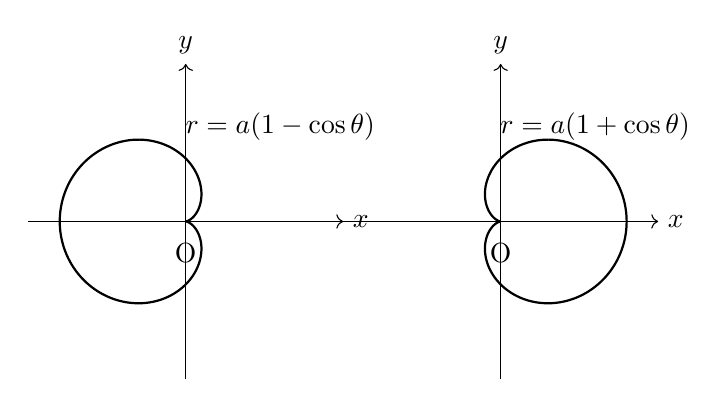
\begin{tikzpicture}[scale=0.8]
			% 左边:r = a(1 - cosθ)
			\begin{scope}[shift={(0,0)}]
				\draw[->] (-2.5,0) -- (2.5,0) node[right] {$x$};
				\draw[->] (0,-2.5) -- (0,2.5) node[above] {$y$};
				\draw[thick, samples=200, domain=0:360] 
				plot ({(1 - cos(\x)) * cos(\x)}, {(1 - cos(\x)) * sin(\x)});
				\node at (0,-0.5) {O};
				\node at (1.5,1.5) {$r = a(1 - \cos\theta)$};
			\end{scope}
			
			% 右边:r = a(1 + cosθ)
			\begin{scope}[shift={(5,0)}]
				\draw[->] (-2.5,0) -- (2.5,0) node[right] {$x$};
				\draw[->] (0,-2.5) -- (0,2.5) node[above] {$y$};
				\draw[thick, samples=200, domain=0:360] 
				plot ({(1 + cos(\x)) * cos(\x)}, {(1 + cos(\x)) * sin(\x)});
				\node at (0,-0.5) {O};
				\node at (1.5,1.5) {$r = a(1 + \cos\theta)$};
			\end{scope}
		\end{tikzpicture}
		
		\subsubsection*{双纽线}
		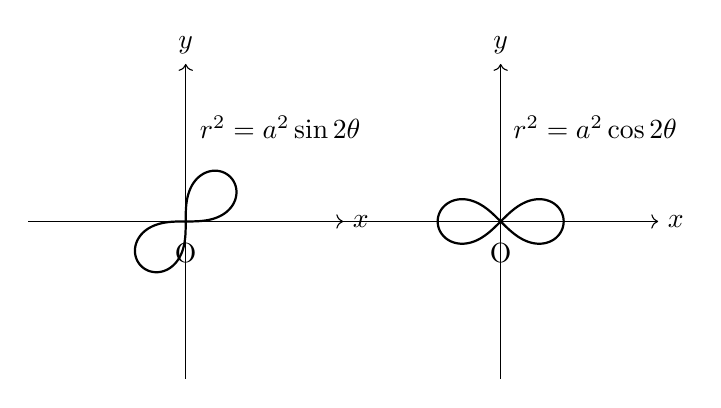
\begin{tikzpicture}[scale=0.8]
			% 左边:r^2 = a^2 sin2θ
			\begin{scope}[shift={(0,0)}]
				\draw[->] (-2.5,0) -- (2.5,0) node[right] {$x$};
				\draw[->] (0,-2.5) -- (0,2.5) node[above] {$y$};
				\draw[thick, samples=200, domain=0:90] 
				plot ({sqrt(sin(2*\x)) * cos(\x)}, {sqrt(sin(2*\x)) * sin(\x)});
				\draw[thick, samples=200, domain=180:270] 
				plot ({sqrt(sin(2*\x)) * cos(\x)}, {sqrt(sin(2*\x)) * sin(\x)});
				\node at (0,-0.5) {O};
				\node at (1.5,1.5) {$r^{2} = a^{2}\sin 2\theta$};
			\end{scope}
			
			% 右边:r^2 = a^2 cos2θ
			\begin{scope}[shift={(5,0)}]
				\draw[->] (-2.5,0) -- (2.5,0) node[right] {$x$};
				\draw[->] (0,-2.5) -- (0,2.5) node[above] {$y$};
				\draw[thick, samples=200, domain=-45:45] 
				plot ({sqrt(cos(2*\x)) * cos(\x)}, {sqrt(cos(2*\x)) * sin(\x)});
				\draw[thick, samples=200, domain=135:225] 
				plot ({sqrt(cos(2*\x)) * cos(\x)}, {sqrt(cos(2*\x)) * sin(\x)});
				\node at (0,-0.5) {O};
				\node at (1.5,1.5) {$r^{2} = a^{2}\cos 2\theta$};
			\end{scope}
		\end{tikzpicture}
		
		\subsubsection*{摆线}

		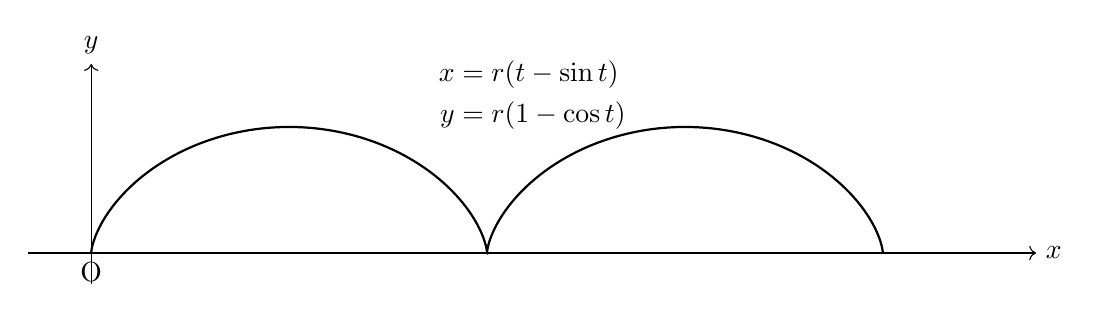
\begin{tikzpicture}[scale=0.8]
			% 左边:一个周期的摆线
			\begin{scope}[shift={(0,0)}]
				\draw[->] (-1,0) -- (15,0) node[right] {$x$};
				\draw[->] (0,-0.5) -- (0,3) node[above] {$y$};
				
				% 绘制两个周期的摆线
				\draw[thick, samples=200, domain=0:4*pi, smooth] 
				plot ({\x - sin(deg(\x))}, {1 - cos(deg(\x))});
				
				% 标记原点
				\node at (0,-0.3) {O};
				
				% 添加公式说明
				\node at (7,2.5) {
					$\begin{aligned}
						x &= r(t - \sin t) \\
						y &= r(1 - \cos t)
					\end{aligned}$
				};
			\end{scope}
		\end{tikzpicture}
	
	\subsubsection*{星形线}
	\begin{tikzpicture}[scale=2]
		% 坐标轴
		\draw[->] (-1.5,0) -- (1.5,0) node[right] {$x$};
		\draw[->] (0,-1.5) -- (0,1.5) node[above] {$y$};
		
		% 星形线
		\draw[thick, domain=0:2*pi, samples=100, smooth, variable=\t]
		plot ({cos(\t r)^3}, {sin(\t r)^3});
		
		% 标记原点
		\node at (0,0) [below left] {$O$};
		
		% 参数方程说明
		\node at (1.8,1.2) {
			$\begin{aligned}
				x &= a \cos^3 t \\
				y &= a \sin^3 t
			\end{aligned}$
		};
	\end{tikzpicture}
	
	\subsubsection*{螺旋线}
	\begin{tikzpicture}[scale=2]
		% 坐标轴
		\draw[->] (-1.5,0) -- (1.5,0) node[right] {$x$};
		\draw[->] (0,-1.5) -- (0,1.5) node[above] {$y$};
		
		% 螺旋线
		\draw[thick, domain=0:4*pi, samples=500, smooth, variable=\t]
		plot ({\t r}: {\t/10});
		
		% 标记原点
		\node at (0,0) [below left] {$O$};
		
		% 极坐标方程说明
		\node at (1.8,1.2) {$r = a \theta$};
	\end{tikzpicture}
	
	\subsection{不同坐标系下的表示}
	直角坐标系下的二重积分表示:
	\[
	\iint_{D} f(x,y) \mathrm{d}\sigma = \iint_{D} f(x,y) \mathrm{d}x\mathrm{d}y
	\]
	极坐标系下的二重积分表示:
	\[
	\iint_{D} f(x,y) \mathrm{d}\sigma = \iint_{D} f(r\cos\theta, r\sin\theta) r \mathrm{d}r\mathrm{d}\theta
	\]
	
	\subsection{二重积分的普通对称性}
	\begin{enumerate}
		\item 如果积分区域 \(D\) 关于 \(x\) 轴对称,则二重积分
		\[
		\iint_{D} f(x,y) \mathrm{d}\sigma = 
		\begin{cases}
			0, & f(x,-y)=-f(x,y)\\
			2\iint_{D_1} f(x,y) \mathrm{d}\sigma, & f(x,-y)=f(x,y)
		\end{cases}
		\]
		其中,\(D_1\) 为 \(D\) 在 \(y\geq0\) 的部分。
		\item 如果积分区域 \(D\) 关于 \(y\) 轴对称,则二重积分
		\[
		\iint_{D} f(x,y) \mathrm{d}\sigma = 
		\begin{cases}
			0, & f(-x,y)=-f(x,y)\\
			2\iint_{D_1} f(x,y) \mathrm{d}\sigma, & f(-x,y)=f(x,y)
		\end{cases}
		\]
		其中,\(D_1\) 为 \(D\) 在 \(x\geq0\) 的部分。
		\item 如果 \(D\) 关于直线 \(y = x\) 对称,则
		\[
		\iint_{D} f(x,y) \mathrm{d}\sigma = \iint_{D} f(y,x) \mathrm{d}\sigma = \frac{1}{2}\iint_{D} (f(x,y)+f(y,x)) \mathrm{d}\sigma
		\]
	\end{enumerate}
	
	\subsection{轮换对称性}
	若将 \(D\) 中的 \(x, y\) 对调后,\(D\) 不变,则有
	\[
	I = \iint_{D} f(x,y) \mathrm{d}x\mathrm{d}y = \iint_{D} f(y,x) \mathrm{d}x\mathrm{d}y
	\]
	
	\subsection{和式极限}
	\[
	\iint_{D} f(x,y) \mathrm{d}\sigma = \lim_{n \to \infty} \sum_{i = 1}^{n} \sum_{j = 1}^{n} f\left(a + \frac{b - a}{n}i, c + \frac{d - c}{n}j\right) \cdot \frac{b - a}{n} \cdot \frac{d - c}{n}
	\]
	这里的 \(D\) 不是一般的平面有界闭区域,而是一个长方形区域 \([a,b] \times [c,d]\)。
	
	\subsection{几何应用}
	曲顶为 \(z = z(x,y)\),\((x,y) \in D_{xy}\) 的柱体体积
	\[
	V = \iint_{D_{xy}} |z(x,y)| \mathrm{d}\sigma
	\]
	总质量
	\[
	m = \iint_{D} \rho(x,y) \mathrm{d}\sigma
	\]
	重心坐标
	\[
	\overline{x} = \frac{\iint_{D} x\rho(x,y) \mathrm{d}\sigma}{\iint_{D} \rho(x,y) \mathrm{d}\sigma}, \quad \overline{y} = \frac{\iint_{D} y\rho(x,y) \mathrm{d}\sigma}{\iint_{D} \rho(x,y) \mathrm{d}\sigma}
	\]
	
	\section{第七章~~~无穷级数 - 数项级数的性质}
		
		\subsection{数项级数的性质}
		\begin{enumerate}
			\item 设 \(c\) 为非零常数,则 \(\sum_{n = 1}^{\infty} u_n\) 与 \(\sum_{n = 1}^{\infty} cu_n\) 有相同的敛散性。
			\item 设有两个级数 \(\sum_{n = 1}^{\infty} u_n\) 与 \(\sum_{n = 1}^{\infty} v_n\),
			\begin{itemize}
				\item 若 \(\sum_{n = 1}^{\infty} u_n = s\),\(\sum_{n = 1}^{\infty} v_n = \sigma\),则 \(\sum_{n = 1}^{\infty} (u_n \pm v_n)=s \pm \sigma\)。
				\item 若 \(\sum_{n = 1}^{\infty} u_n\) 收敛,\(\sum_{n = 1}^{\infty} v_n\) 发散,则 \(\sum_{n = 1}^{\infty} (u_n \pm v_n)\) 发散。
				\item 若 \(\sum_{n = 1}^{\infty} u_n\),\(\sum_{n = 1}^{\infty} v_n\) 均发散,则 \(\sum_{n = 1}^{\infty} (u_n \pm v_n)\) 敛散性不定。
			\end{itemize}
			\item 添加、去掉或改变有限项不影响级数的敛散性。
			\item 设级数 \(\sum_{n = 1}^{\infty} u_n\) 收敛,则对其各项任意加括号后所得新级数仍收敛于原级数的和。
			\begin{remark}
				\item 一个级数加括号所得新级数发散,则原级数发散。
				\item 一个级数加括号后收敛,原级数的敛散性不定。
			\end{remark}
			\item 级数 \(\sum_{n = 1}^{\infty} u_n\) 收敛的必要条件:\(\lim_{n \to \infty} u_n = 0\)。
		\end{enumerate}
		
		\subsection{常见级数的敛散性}
		\begin{enumerate}
			\item 等比级数 \(\sum_{n = 1}^{\infty} aq^{n - 1}=
			\begin{cases}
				\frac{a}{1 - q}, & |q| < 1\\
				\text{发散}, & |q| \geq 1
			\end{cases}\)
			\item \(p\) - 级数 \(\sum_{n = 1}^{\infty} \frac{1}{n^{p}} = 
			\begin{cases}
				\text{收敛}, & p > 1\\
				\text{发散}, & p \leq 1
			\end{cases}\)
			\item \(\sum_{n = 2}^{\infty} \frac{1}{n\ln^{p}n}=
			\begin{cases}
				\text{收敛}, & p > 1\\
				\text{发散}, & p \leq 1
			\end{cases}\)
		\end{enumerate}
		
		\subsection{正项级数的敛散性判别方法}
		(1)比较判别法
		
		设 \(0\leq u_n\leq v_n\),若 \(\sum_{n = 1}^{\infty} v_n\) 收敛,则 \(\sum_{n = 1}^{\infty} u_n\) 收敛。若 \(\sum_{n = 1}^{\infty} u_n\) 发散,则 \(\sum_{n = 1}^{\infty} v_n\) 发散。
		
		(2)比较判别法的极限形式
		
		设 \(\sum_{n = 1}^{\infty} u_n\) 及 \(\sum_{n = 1}^{\infty} v_n\) 均为正项级数,且 \(\lim_{n \to \infty} \frac{u_n}{v_n}=A (v_n\neq0)\)。
		\begin{enumerate}
			\item 若 \(0\leq A<+\infty\),且 \(\sum_{n = 1}^{\infty} v_n\) 收敛,则 \(\sum_{n = 1}^{\infty} u_n\) 收敛。
			\item 若 \(0 < A\leq+\infty\),且 \(\sum_{n = 1}^{\infty} v_n\) 发散,则 \(\sum_{n = 1}^{\infty} u_n\) 发散。
		\end{enumerate}
		
		(3)比值判别法(达朗贝尔准则)(适用于通项 \(u_n\) 中含有 \(n!\) 或关于 \(n\) 的若干连乘形式)
		
		设 \(u_n\geq0\),\(n = 1, 2, \cdots\),对于 \(\sum_{n = 1}^{\infty} u_n\) ,有 \(\lim_{n \to \infty} \frac{u_{n + 1}}{u_n}=\rho\)
		\[
		\begin{cases}
			\rho>1\text{ 时}, & \sum_{n = 1}^{\infty} u_n\text{ 发散}\\
			\rho = 1\text{ 时}, & \text{方法失效}\\
			\rho<1\text{ 时}, & \sum_{n = 1}^{\infty} u_n\text{ 收敛}
		\end{cases}
		\]
		
		(4)根值判别法(适用于 \(u_n\) 中含有以 \(n\) 为指数幂的因子)
		
		设 \(u_n\geq0\),\(n = 1, 2, \cdots\),对 \(\sum_{n = 1}^{\infty} u_n\) ,有 \(\lim_{n \to \infty} \sqrt[n]{u_n}=\rho\)
		\[
		\begin{cases}
			\rho>1\text{ 时}, & \sum_{n = 1}^{\infty} u_n\text{ 发散}\\
			\rho = 1\text{ 时}, & \text{方法失效}\\
			\rho<1\text{ 时}, & \sum_{n = 1}^{\infty} u_n\text{ 收敛}
		\end{cases}
		\]
		
		\subsection{交错级数判敛方法(莱布尼茨准则)}
		若交错级数 \(\sum_{n = 1}^{\infty} (-1)^{n - 1}u_n (u_n>0)\) 满足条件:
		\begin{enumerate}
			\item \(u_n\geq u_{n + 1}\),\((n = 1, 2, \cdots)\)
			\item \(\lim_{n \to \infty} u_n = 0\)
		\end{enumerate}
		则交错级数收敛,其和 \(S\leq u_1\),余项 \(|R_n|\leq u_{n + 1}\)。
		
		\subsection{幂级数收敛半径、收敛区间}
		设幂级数 \(\sum_{n = 0}^{\infty} a_nx^n\),其系数当 \(n\geq N\) 时 \(a_n\neq0\),且 \(\lim_{n \to \infty} \left|\frac{a_{n + 1}}{a_n}\right|=\rho\),
		则收敛半径 \(R = 
		\begin{cases}
			1/\rho, & 0 < \rho < +\infty\\
			+\infty, & \rho = 0\\
			0, & \rho = +\infty
		\end{cases}\)
		\((-R, R)\) 为其收敛区间。
		
		阿贝尔定理
		
		当幂级数 \(\sum_{n = 0}^{\infty} a_nx^n\) 在点 \(x = x_1 (x_1\neq0)\) 处收敛时,对于满足 \(|x| < |x_1|\) 的一切 \(x\),幂级数绝对收敛;当幂级数 \(\sum_{n = 0}^{\infty} a_nx^n\) 在点 \(x = x_2 (x_2\neq0)\) 处发散时,对于满足 \(|x| > |x_2|\) 的一切 \(x\),幂级数发散。
		
		\subsection{常用的函数展开式}
		\begin{enumerate}
			\item \(\frac{1}{1 - x}=1 + x + x^2+\cdots + x^n+\cdots=\sum_{n = 0}^{\infty} x^n\),\(x\in(-1,1)\)。
			\item \(\frac{1}{1 + x}=1 - x + x^2-\cdots + (-1)^nx^n+\cdots=\sum_{n = 0}^{\infty} (-1)^nx^n\),\(x\in(-1,1)\)。
			\item \(e^x=1 + x+\frac{x^2}{2!}+\cdots+\frac{x^n}{n!}+\cdots=\sum_{n = 0}^{\infty} \frac{x^n}{n!}\),\(x\in(-\infty,+\infty)\)。
			\item \(\sin x=x-\frac{x^3}{3!}+\cdots+(-1)^n\frac{x^{2n + 1}}{(2n + 1)!}+\cdots=\sum_{n = 0}^{\infty} (-1)^n\frac{x^{2n + 1}}{(2n + 1)!}\),\(x\in(-\infty,+\infty)\)。
			\item \(\cos x=1-\frac{x^2}{2!}+\frac{x^4}{4!}-\cdots+(-1)^n\frac{x^{2n}}{(2n)!}+\cdots=\sum_{n = 0}^{\infty} (-1)^n\frac{x^{2n}}{(2n)!}\),\(x\in(-\infty,+\infty)\)。
			\item \(\ln(1 + x)=x-\frac{x^2}{2}+\frac{x^3}{3}-\cdots+(-1)^n\frac{x^{n + 1}}{n + 1}+\cdots=\sum_{n = 0}^{\infty} (-1)^n\frac{x^{n + 1}}{n + 1}\),\(x\in(-1,1]\)。
			\item \((1 + x)^a=1 + ax+\frac{a(a - 1)}{2!}x^2+\cdots+\frac{a(a - 1)\cdots(a - n + 1)}{n!}x^n+\cdots\),\(x\in(-1,1)\)。
		\end{enumerate}
		
		\subsection{傅里叶级数狄利克雷收敛定理}
		设函数 \(f(x)\) 是以 \(2l\) 为周期的周期函数,在 \([-l, l]\) 上满足条件:
		\begin{enumerate}
			\item 除有限个第一类间断点外都连续;
			\item 只有有限个极值点。
		\end{enumerate}
		则 \(f(x)\) 的傅里叶级数在 \([-l, l]\) 上收敛,且和函数
		\[
		s(x)=
		\begin{cases}
			f(x), & x_0为f(x)的连续点\\
			\frac{1}{2}[f(x_0 - 0)+f(x_0 + 0)], & x_0为f(x)的间断点
		\end{cases}
		\]
		
		\subsection{傅里叶级数系数公式}
		\[
		f(x)\sim\frac{a_0}{2}+\sum_{n = 1}^{\infty}\left(a_n\cos\frac{n\pi x}{l}+b_n\sin\frac{n\pi x}{l}\right)
		\]
		其中
		\[
		\begin{cases}
			a_0=\frac{1}{l}\int_{-l}^{l}f(x)\mathrm{d}x\\
			a_n=\frac{1}{l}\int_{-l}^{l}f(x)\cos\frac{n\pi x}{l}\mathrm{d}x, & n = 1, 2, \cdots\\
			b_n=\frac{1}{l}\int_{-l}^{l}f(x)\sin\frac{n\pi x}{l}\mathrm{d}x
		\end{cases}
		\]
		\begin{enumerate}
			\item 当 \(f(x)\) 为奇函数时,其展开式是正弦级数
			\[
			f(x)\sim\sum_{n = 1}^{\infty}b_n\sin\frac{n\pi x}{l}, \quad b_n=\frac{2}{l}\int_{0}^{l}f(x)\sin\frac{n\pi x}{l}\mathrm{d}x, \quad n = 1, 2, \cdots
			\]
			\item 当 \(f(x)\) 为偶函数时,其展开式是余弦级数
			\[
			f(x)\sim\frac{a_0}{2}+\sum_{n = 1}^{\infty}a_n\cos\frac{n\pi x}{l}
			\]
			其中 \(a_0=\frac{2}{l}\int_{0}^{l}f(x)\mathrm{d}x\),\(a_n=\frac{2}{l}\int_{0}^{l}f(x)\cos\frac{n\pi x}{l}\mathrm{d}x\),\(n = 1, 2, \cdots\)
		\end{enumerate}
		
		\section{第八章~~~向量代数、空间几何与场论初步 - 向量代数运算}
			
			\subsection{向量代数运算}
			(1)向量 \(\vec{a}\) 的方向余弦
			
			设向量的坐标表示为 \(\vec{a}=x\vec{i}+y\vec{j}+z\vec{k}=(x,y,z)\)。
			\[
			\cos\alpha=\frac{x}{\sqrt{x^{2}+y^{2}+z^{2}}}, \quad \cos\beta=\frac{y}{\sqrt{x^{2}+y^{2}+z^{2}}}, \quad \cos\gamma=\frac{z}{\sqrt{x^{2}+y^{2}+z^{2}}}
			\]
			
			(2)数量积(点积,内积)
			
			设 \(\vec{a}=(x_1,y_1,z_1)\),\(\vec{b}=(x_2,y_2,z_2)\),则向量 \(\vec{a}\) 与 \(\vec{b}\) 的数量积为
			\[
			\vec{a}\cdot\vec{b}=|\vec{a}||\vec{b}|\cos\langle\vec{a},\vec{b}\rangle=x_1x_2 + y_1y_2 + z_1z_2
			\]
			
			(3)向量积(叉积,外积)
			
			设两向量 \(\vec{a}\) 与 \(\vec{b}\),若存在一个向量 \(\vec{c}\),满足条件:
			\begin{enumerate}
				\item \(|\vec{c}|=|\vec{a}||\vec{b}|\sin\langle\vec{a},\vec{b}\rangle\);
				\item \(\vec{c}\perp\vec{a}\),\(\vec{c}\perp\vec{b}\),即 \(\vec{c}\) 垂直于 \(\vec{a}\),\(\vec{b}\) 所确定的平面;
				\item \(\vec{a}\),\(\vec{b}\),\(\vec{c}\) 成右手系。
			\end{enumerate}
			则向量 \(\vec{c}\) 称为向量 \(\vec{a}\) 与 \(\vec{b}\) 的向量积,记为 \(\vec{c}=\vec{a}\times\vec{b}\),利用坐标可表示为
			\[
			\vec{a}\times\vec{b}=
			\begin{vmatrix}
				\vec{i} & \vec{j} & \vec{k}\\
				x_1 & y_1 & z_1\\
				x_2 & y_2 & z_2
			\end{vmatrix}
			=
			\begin{vmatrix}
				y_1 & z_1\\
				y_2 & z_2
			\end{vmatrix}\vec{i}-
			\begin{vmatrix}
				x_1 & z_1\\
				x_2 & z_2
			\end{vmatrix}\vec{j}+
			\begin{vmatrix}
				x_1 & y_1\\
				x_2 & y_2
			\end{vmatrix}\vec{k}
			\]
			
			(4)混合积
			
			设有三个向量 \(\vec{a}=(x_1,y_1,z_1)\),\(\vec{b}=(x_2,y_2,z_2)\),\(\vec{c}=(x_3,y_3,z_3)\),先作 \(\vec{a}\),\(\vec{b}\) 的向量积 \(\vec{a}\times\vec{b}\),再与 \(\vec{c}\) 作数量积 \((\vec{a}\times\vec{b})\cdot\vec{c}\),则其称为 \(\vec{a}\),\(\vec{b}\),\(\vec{c}\) 的混合积,记为 \([\vec{a},\vec{b},\vec{c}]\),利用坐标可表示为
			\[
			[\vec{a},\vec{b},\vec{c}]=(\vec{a}\times\vec{b})\cdot\vec{c}=
			\begin{vmatrix}
				x_1 & y_1 & z_1\\
				x_2 & y_2 & z_2\\
				x_3 & y_3 & z_3
			\end{vmatrix}
			\]
			\begin{remark}
				\(|\vec{[a},\vec{b},\vec{c}]|\) 表示以 \(\vec{a}\),\(\vec{b}\),\(\vec{c}\) 为棱的平行六面体体积,注意不要忘记绝对值号。
			\end{remark}
			
			
			\subsection{直线与平面方程}
			\subsubsection{平面方程}
			\subsubsection*{一般式}
			\[ Ax + By + Cz + D = 0 \]
			
			\subsubsection*{点法式}
			平面过 \((x_0, y_0, z_0)\) 点,法向量为 \(\boldsymbol{n} = (A, B, C)\),方程为:  
			\[ A(x - x_0) + B(y - y_0) + C(z - z_0) = 0 \]
			
			\subsubsection*{截距式}
			\[ \frac{x}{a} + \frac{y}{b} + \frac{z}{c} = 1 \]
			
			\subsubsection{空间直线方程}
			\subsubsection*{一般式}
			\[ \begin{cases} 
				A_1x + B_1y + C_1z + D_1 = 0, \\
				A_2x + B_2y + C_2z + D_2 = 0 
			\end{cases} \]
			
			\subsubsection*{参数式}
			直线过 \((x_0, y_0, z_0)\),方向向量为 \(\boldsymbol{s} = (l, m, n)\),方程为:  
			\[ \begin{cases} 
				x = x_0 + lt, \\ 
				y = y_0 + mt, \\ 
				z = z_0 + nt 
			\end{cases} \]
			
			\subsubsection*{标准式(对称式)}
			过 \((x_0, y_0, z_0)\),方向向量为 \(\boldsymbol{s} = (l, m, n)\),方程为:  
			\[ \frac{x - x_0}{l} = \frac{y - y_0}{m} = \frac{z - z_0}{n} \]
			
			\subsubsection{平面间、直线间、直线与平面间关系}
			设平面 \(\pi_1, \pi_2\),直线 \(L_1, L_2\) 方程如下:  
			
			\subsubsection*{平面方程与法向量}
		平面 \(\pi_1\):\(A_1x + B_1y + C_1z + D_1 = 0\),法向量 \(\boldsymbol{n_1} = (A_1, B_1, C_1)\)  
			
		平面 \(\pi_2\):\(A_2x + B_2y + C_2z + D_2 = 0\),法向量 \(\boldsymbol{n_2} = (A_2, B_2, C_2)\)  
			
			\subsubsection*{直线方程与方向向量}
		直线 \(L_1\):\(\frac{x - x_1}{l_1} = \frac{y - y_1}{m_1} = \frac{z - z_1}{n_1}\),方向向量 \(\boldsymbol{s_1} = (l_1, m_1, n_1)\)  
			
		直线 \(L_2\):\(\frac{x - x_2}{l_2} = \frac{y - y_2}{m_2} = \frac{z - z_2}{n_2}\),方向向量 \(\boldsymbol{s_2} = (l_2, m_2, n_2)\)  
			
			\subsection{直线与平面方程}
			\subsubsection{平面方程}
			\subsubsection*{一般式}
			\[ Ax + By + Cz + D = 0 \]
			
			\subsubsection*{点法式}
			平面过 \((x_0, y_0, z_0)\) 点,法向量为 \(\boldsymbol{n} = (A, B, C)\),方程为:  
			\[ A(x - x_0) + B(y - y_0) + C(z - z_0) = 0 \]
			
			\subsubsection*{截距式}
			\[ \frac{x}{a} + \frac{y}{b} + \frac{z}{c} = 1 \]
			
			\subsubsection{空间直线方程}
			\subsubsection*{一般式}
			\[ \begin{cases} 
				A_1x + B_1y + C_1z + D_1 = 0, \\
				A_2x + B_2y + C_2z + D_2 = 0 
			\end{cases} \]
			
			\subsubsection*{参数式}
			直线过 \((x_0, y_0, z_0)\),方向向量为 \(\boldsymbol{s} = (l, m, n)\),方程为:  
			\[ \begin{cases} 
				x = x_0 + lt, \\ 
				y = y_0 + mt, \\ 
				z = z_0 + nt 
			\end{cases} \]
			
			\subsubsection*{标准式(对称式)}
			过 \((x_0, y_0, z_0)\),方向向量为 \(\boldsymbol{s} = (l, m, n)\),方程为:  
			\[ \frac{x - x_0}{l} = \frac{y - y_0}{m} = \frac{z - z_0}{n} \]
			
			\subsubsection{平面间、直线间、直线与平面间关系}
			\subsubsection*{两平面 \(\pi_1, \pi_2\) 间的位置关系}
			设平面 \(\pi_1: A_1x + B_1y + C_1z + D_1 = 0\)(法向量 \(\boldsymbol{n_1} = (A_1, B_1, C_1)\)),  
			平面 \(\pi_2: A_2x + B_2y + C_2z + D_2 = 0\)(法向量 \(\boldsymbol{n_2} = (A_2, B_2, C_2)\))。  
			
			\paragraph{平行}  
			\[ \pi_1 \parallel \pi_2 \Leftrightarrow \boldsymbol{n_1} \parallel \boldsymbol{n_2} \Leftrightarrow \frac{A_1}{A_2} = \frac{B_1}{B_2} = \frac{C_1}{C_2} \Leftrightarrow \boldsymbol{n_1} \times \boldsymbol{n_2} = \boldsymbol{0} \]  
			
			\paragraph{垂直}  
			\[ \pi_1 \perp \pi_2 \Leftrightarrow \boldsymbol{n_1} \perp \boldsymbol{n_2} \Leftrightarrow A_1A_2 + B_1B_2 + C_1C_2 = 0 \Leftrightarrow \boldsymbol{n_1} \cdot \boldsymbol{n_2} = 0 \]  
			
			\paragraph{夹角 \(\theta\)(\(0 \leqslant \theta \leqslant \frac{\pi}{2}\))}  
			\[ \cos\theta = \frac{|\boldsymbol{n_1} \cdot \boldsymbol{n_2}|}{|\boldsymbol{n_1}| \cdot |\boldsymbol{n_2}|} = \frac{|A_1A_2 + B_1B_2 + C_1C_2|}{\sqrt{A_1^2 + B_1^2 + C_1^2} \cdot \sqrt{A_2^2 + B_2^2 + C_2^2}} \]  
			
			
			\subsubsection*{两直线 \(L_1, L_2\) 间的位置关系}
			设直线 \(L_1: \frac{x - x_1}{l_1} = \frac{y - y_1}{m_1} = \frac{z - z_1}{n_1}\)(方向向量 \(\boldsymbol{s_1} = (l_1, m_1, n_1)\)),  
			直线 \(L_2: \frac{x - x_2}{l_2} = \frac{y - y_2}{m_2} = \frac{z - z_2}{n_2}\)(方向向量 \(\boldsymbol{s_2} = (l_2, m_2, n_2)\))。  
			
			\paragraph{平行}  
			\[ L_1 \parallel L_2 \Leftrightarrow \boldsymbol{s_1} \parallel \boldsymbol{s_2} \Leftrightarrow \frac{l_1}{l_2} = \frac{m_1}{m_2} = \frac{n_1}{n_2} \Leftrightarrow \boldsymbol{s_1} \times \boldsymbol{s_2} = \boldsymbol{0} \]  
			
			\paragraph{垂直}  
			\[ L_1 \perp L_2 \Leftrightarrow \boldsymbol{s_1} \perp \boldsymbol{s_2} \Leftrightarrow l_1l_2 + m_1m_2 + n_1n_2 = 0 \Leftrightarrow \boldsymbol{s_1} \cdot \boldsymbol{s_2} = 0 \]  
			
			\paragraph{夹角 \(\theta\)(\(0 \leqslant \theta \leqslant \frac{\pi}{2}\))}  
			\[ \cos\theta = \frac{|\boldsymbol{s_1} \cdot \boldsymbol{s_2}|}{|\boldsymbol{s_1}| \cdot |\boldsymbol{s_2}|} = \frac{|l_1l_2 + m_1m_2 + n_1n_2|}{\sqrt{l_1^2 + m_1^2 + n_1^2} \cdot \sqrt{l_2^2 + m_2^2 + n_2^2}} \]  
			
			
			\subsubsection*{直线 \(L_1\) 与平面 \(\pi_1\) 间的位置关系}
			设直线 \(L_1: \frac{x - x_1}{l_1} = \frac{y - y_1}{m_1} = \frac{z - z_1}{n_1}\)(方向向量 \(\boldsymbol{s_1} = (l_1, m_1, n_1)\)),  
			平面 \(\pi_1: A_1x + B_1y + C_1z + D_1 = 0\)(法向量 \(\boldsymbol{n_1} = (A_1, B_1, C_1)\))。  
			
			\paragraph{直线平行于平面}  
			\[ L_1 \parallel \pi_1 \Leftrightarrow \boldsymbol{s_1} \perp \boldsymbol{n_1} \Leftrightarrow A_1l_1 + B_1m_1 + C_1n_1 = 0 \Leftrightarrow \boldsymbol{s_1} \cdot \boldsymbol{n_1} = 0 \]  
			
			\paragraph{直线垂直于平面}  
			\[ L_1 \perp \pi_1 \Leftrightarrow \boldsymbol{s_1} \parallel \boldsymbol{n_1} \Leftrightarrow \frac{A_1}{l_1} = \frac{B_1}{m_1} = \frac{C_1}{n_1} \Leftrightarrow \boldsymbol{s_1} \times \boldsymbol{n_1} = \boldsymbol{0} \]  
			
			\paragraph{夹角 \(\theta\)(\(0 \leqslant \theta \leqslant \frac{\pi}{2}\))}  
			\[ \sin\theta = \frac{|\boldsymbol{s_1} \cdot \boldsymbol{n_1}|}{|\boldsymbol{s_1}| \cdot |\boldsymbol{n_1}|} = \frac{|A_1l_1 + B_1m_1 + C_1n_1|}{\sqrt{l_1^2 + m_1^2 + n_1^2} \cdot \sqrt{A_1^2 + B_1^2 + C_1^2}} \]  
			
			
			\subsubsection*{点到平面的距离}
			点 \(M(x_0, y_0, z_0)\) 到平面 \(Ax + By + Cz + D = 0\) 的距离:  
			\[ d = \frac{|Ax_0 + By_0 + Cz_0 + D|}{\sqrt{A^2 + B^2 + C^2}} \]  
			
			
			\subsection{空间曲线}
			\subsubsection{旋转曲面}
			设 \( L \) 是平面 \( zOx \) 上的一条曲线,其方程为:  
			\[ \begin{cases} 
				f(x, z) = 0, \\ 
				y = 0 
			\end{cases} \]  
			
			\subsubsection*{绕 \( x \) 轴旋转}  
			\( L \) 绕 \( x \) 轴旋转一周产生的旋转面方程:  
			\[ f\left(x, \pm \sqrt{y^2 + z^2}\right) = 0 \]  
			
			\subsubsection*{绕 \( z \) 轴旋转}  
			\( L \) 绕 \( z \) 轴旋转一周产生的旋转面方程:  
			\[ f\left(\pm \sqrt{x^2 + y^2}, z\right) = 0 \]  
			
			
			\subsubsection{九类二次曲面}
			\subsubsection*{椭圆锥面}  
			\[ \frac{x^2}{a^2} + \frac{y^2}{b^2} = z^2 \]  
			
			\subsubsection*{椭球面}  
			\[ \frac{x^2}{a^2} + \frac{y^2}{b^2} + \frac{z^2}{c^2} = 1 \]  
			
			\subsubsection*{单叶双曲面}  
			\[ \frac{x^2}{a^2} + \frac{y^2}{b^2} - \frac{z^2}{c^2} = 1 \]  
			
			\subsubsection*{双叶双曲面}  
			\[ \frac{x^2}{a^2} - \frac{y^2}{b^2} - \frac{z^2}{c^2} = 1 \]  
			
			\subsubsection*{椭圆抛物面}  
			\[ \frac{x^2}{a^2} + \frac{y^2}{b^2} = \pm z \]  
			
			\subsubsection*{双曲抛物面}  
			\[ \frac{x^2}{a^2} - \frac{y^2}{b^2} = \pm z \]  
			
			\subsubsection*{椭圆柱面}  
			\[ \frac{x^2}{a^2} + \frac{y^2}{b^2} = 1 \]  
			
			\subsubsection*{双曲柱面}  
			\[ \frac{x^2}{a^2} - \frac{y^2}{b^2} = 1 \]  
			
			\subsubsection*{抛物柱面}  
			\[ x^2 = ay \]  
			
			
			\subsection{空间曲线在坐标轴上的投影}
			空间曲线在坐标面上的投影曲线,称为曲线在坐标面上的投影。  
			
			设空间曲线 \( L \) 的一般方程:  
			\[ \begin{cases} 
				F(x, y, z) = 0, \\ 
				G(x, y, z) = 0 
			\end{cases} \]  
			
			消去 \( z \) 得投影柱面方程 \( H(x, y) = 0 \),则 \( L \) 在 \( xOy \) 平面上投影曲线的方程:  
			\[ \begin{cases} 
				H(x, y) = 0, \\ 
				z = 0 
			\end{cases} \]  
			
			
			\subsection{空间曲线的切线及法平面方程}
			空间曲线 \( \Gamma \) 的参数方程:  
			\[ \begin{cases} 
				x = x(t), \\ 
				y = y(t), \\ 
				z = z(t) 
			\end{cases} \]  
			
			\( \Gamma \) 在点 \( (x_0, y_0, z_0) \)(对应参数 \( t = t_0 \))处:  
			
			\subsubsection*{切线方程}  
			\[ \frac{x - x_0}{x'(t_0)} = \frac{y - y_0}{y'(t_0)} = \frac{z - z_0}{z'(t_0)} \]  
			
			\subsubsection*{法平面方程}  
			\[ x'(t_0)(x - x_0) + y'(t_0)(y - y_0) + z'(t_0)(z - z_0) = 0 \]  
			
			
			\subsection{空间曲面在其点上某点处的切平面和法线方程}
			设曲面 \( \Sigma \) 的方程为 \( F(x, y, z) = 0 \),在 \( \Sigma \) 上一点 \( (x_0, y_0, z_0) \) 处:  
			
			\subsubsection*{切平面方程}  
			\[ F_x'\big|_{(x_0,y_0,z_0)} (x - x_0) + F_y'\big|_{(x_0,y_0,z_0)} (y - y_0) + F_z'\big|_{(x_0,y_0,z_0)} (z - z_0) = 0 \]  
			
			\subsubsection*{法线方程}  
			\[ \frac{x - x_0}{F_x'\big|_{(x_0,y_0,z_0)}} = \frac{y - y_0}{F_y'\big|_{(x_0,y_0,z_0)}} = \frac{z - z_0}{F_z'\big|_{(x_0,y_0,z_0)}} \]  
			
			
			\subsection{方向导数与梯度}
			\subsubsection*{方向导数}
			函数在点 \( (x_0, y_0) \) 沿方向 \( l \)(方向余弦 \( (\cos\alpha, \cos\beta) \))的方向导数:  
			\[ \left. \frac{\partial f}{\partial l} \right|_{(x_0,y_0)} = f_x'(x_0, y_0) \cos\alpha + f_y'(x_0, y_0) \cos\beta \]  
			
			
			\subsubsection*{梯度}
			函数在点 \( (x_0, y_0) \) 处的梯度:  
			\[ \text{grad}f(x_0, y_0) = f_x'(x_0, y_0) \boldsymbol{i} + f_y'(x_0, y_0) \boldsymbol{j} \]  
			
			\section{第九章~~~三重积分}
			
			\subsection{不同坐标系下的表示}
			\subsubsection{直角坐标系下的三重积分表示}
			
			\begin{align}
				\iiint_{\Omega} f(x, y, z) \mathrm{d}v &= \iint_{D_{xy}} \mathrm{d}x \mathrm{d}y \int_{z_1(x,y)}^{z_2(x,y)} f(x, y, z) \mathrm{d}z \quad \text{(先一后二)} \\
				\iiint_{\Omega} f(x, y, z) \mathrm{d}v &= \int_{c}^{d} \mathrm{d}z \iint_{D_z} f(x, y, z) \mathrm{d}x \mathrm{d}y \quad \text{(先二后一)}
			\end{align}
			
			
			\subsubsection{柱坐标系下的三重积分表示}
			\[ 
			\iiint_{\Omega} f(x, y, z) \mathrm{d}v = \iiint_{\Omega} f(r \cos\theta, r \sin\theta, z) r \mathrm{d}r \mathrm{d}\theta \mathrm{d}z
			\]
			
			\subsubsection{球坐标系下的三重积分表示}
			\[ 
			\iiint_{\Omega} f(x, y, z) \mathrm{d}v = \iiint_{\Omega} f(r \sin\varphi \cos\theta, r \sin\varphi \sin\theta, r \cos\varphi) r^2 \sin\varphi \mathrm{d}r \mathrm{d}\varphi \mathrm{d}\theta
			\]
			
			\subsection{三重积分的普通对称性与轮换对称性}
			\subsubsection{普通对称性(关于 \( xOy \) 面对称)}
			若 \( \Omega \) 关于 \( xOy \) 面对称,则
			\[ 
			\iiint_{\Omega} f(x, y, z) \mathrm{d}v = 
			\begin{cases}
				0, & f(x, y, -z) = -f(x, y, z), \\
				2\iiint_{\Omega_1} f(x, y, z) \mathrm{d}v, & f(x, y, -z) = f(x, y, z).
			\end{cases}
			\]
			其中 \( \Omega_1 \) 是 \( \Omega \) 在 \( xOy \) 面上方部分,关于 \( yOz \),\( xOz \) 面的对称性有类似的性质。
			
			\subsubsection{轮换对称性}
			如果积分区域关于变量 \( x \),\( y \),\( z \) 具有轮换对称性(即将表示积分区域的方程 \( x \) 换成 \( y \),\( y \) 换成 \( z \) 或 \( z \) 换成 \( x \) 后表达式不变),则
			\[ 
			\iiint_{\Omega} f(x, y, z) \mathrm{d}v = \iiint_{\Omega} f(y, z, x) \mathrm{d}v = \iiint_{\Omega} f(z, x, y) \mathrm{d}v
			\]
			
		
			\subsection{换元法求三重积分}
			
			\begin{align*}
				&\iiint_{\Omega_{xyz}} f(x, y, z) \mathrm{d}x \mathrm{d}y \mathrm{d}z \\
				&\stackrel{\substack{x = x(u, v, w)\\y = y(u, v, w)\\z = z(u, v, w)}}{=} \iiint_{\Omega_{uvw}} f[x(u, v, w), y(u, v, w), z(u, v, w)] \left| \frac{\partial(x, y, z)}{\partial(u, v, w)} \right| \mathrm{d}u \mathrm{d}v \mathrm{d}w
			\end{align*}
			
			其中:
			\begin{enumerate}
				\item \( f(x, y, z) \to f[x(u, v, w), y(u, v, w), z(u, v, w)] \)。
				\item \( \iiint_{\Omega_{xyz}} \to \iiint_{\Omega_{uvw}} \)。
				\item \( \mathrm{d}x \mathrm{d}y \mathrm{d}z \to \left| \frac{\partial(x, y, z)}{\partial(u, v, w)} \right| \mathrm{d}u \mathrm{d}v \mathrm{d}w \)。
			\end{enumerate}
			
			\subsection{几何物理应用}
			\subsubsection{体积}
			对于空间物体 \( \Omega \),其体积计算公式为:
			\[ V = \iiint_{\Omega} \mathrm{d}v \]
			
			\subsubsection{总质量}
			对空间物体 \( \Omega \),其体积密度为 \( \rho(x, y, z) \),则其总质量计算公式为:
			\[ m = \iiint_{\Omega} \rho(x, y, z) \mathrm{d}v \]
			
			\subsubsection{重心}
			对空间物体 \( \Omega \),其体积密度为 \( \rho(x, y, z) \),则重心 \( (\overline{x}, \overline{y}, \overline{z}) \) 的计算公式为:
			\[ 
			\overline{x} = \frac{\iiint_{\Omega} x \rho(x, y, z) \mathrm{d}v}{\iiint_{\Omega} \rho(x, y, z) \mathrm{d}v}, \quad
			\overline{y} = \frac{\iiint_{\Omega} y \rho(x, y, z) \mathrm{d}v}{\iiint_{\Omega} \rho(x, y, z) \mathrm{d}v}, \quad
			\overline{z} = \frac{\iiint_{\Omega} z \rho(x, y, z) \mathrm{d}v}{\iiint_{\Omega} \rho(x, y, z) \mathrm{d}v}
			\]
			
			\subsubsection{转动惯量}
			对于空间物体 \( \Omega \),其体积密度为 \( \rho(x, y, z) \),则该物体对 \( x \) 轴、\( y \) 轴、\( z \) 轴和原点 \( O \) 的转动惯量 \( I_x \),\( I_y \),\( I_z \) 和 \( I_O \) 的计算公式分别为:
			 
			\begin{align*}
				I_x &= \iiint_{\Omega} (y^2 + z^2) \rho(x, y, z) \mathrm{d}v, \\
				I_y &= \iiint_{\Omega} (z^2 + x^2) \rho(x, y, z) \mathrm{d}v, \\
				I_z &= \iiint_{\Omega} (x^2 + y^2) \rho(x, y, z) \mathrm{d}v, \\
				I_O &= \iiint_{\Omega} (x^2 + y^2 + z^2) \rho(x, y, z) \mathrm{d}v.
			\end{align*}
			
			
			\subsubsection{引力}
			对于空间物体 \( \Omega \),其体积密度为 \( \rho(x, y, z) \),则该物体对物体外一点 \( M_0(x_0, y_0, z_0) \) 处的质量为 \( m \) 的质点的引力 \( (F_x, F_y, F_z) \) 的计算公式为:
			
			\begin{align*}
				F_x &= Gm \iiint_{\Omega} \frac{\rho(x, y, z)(x - x_0)}{[(x - x_0)^2 + (y - y_0)^2 + (z - z_0)^2]^{\frac{3}{2}}} \mathrm{d}v, \\
				F_y &= Gm \iiint_{\Omega} \frac{\rho(x, y, z)(y - y_0)}{[(x - x_0)^2 + (y - y_0)^2 + (z - z_0)^2]^{\frac{3}{2}}} \mathrm{d}v, \\
				F_z &= Gm \iiint_{\Omega} \frac{\rho(x, y, z)(z - z_0)}{[(x - x_0)^2 + (y - y_0)^2 + (z - z_0)^2]^{\frac{3}{2}}} \mathrm{d}v.
			\end{align*}
			
			\section{第十章~~~曲线曲面积分}
			\subsection{曲线积分化为定积分}
			\subsubsection{曲线 \( L: y = \varphi(x), a \leq x \leq b \) 的情况}
			\begin{enumerate}
				\item 第一类曲线积分
				\[ \int_{L} f(x, y) \mathrm{d}s = \int_{a}^{b} f[x, \varphi(x)] \sqrt{1 + [\varphi'(x)]^2} \mathrm{d}x \]
				\item 第二类曲线积分
				\[ \int_{L} P(x, y) \mathrm{d}x + Q(x, y) \mathrm{d}y = \int_{a}^{b} \{ P[x, \varphi(x)] + Q[x, \varphi(x)]\varphi'(x) \} \mathrm{d}x \]
			\end{enumerate}
			\subsubsection{曲线 \( L: x = x(t), y = y(t), z = z(t) \)(\( a \leq t \leq \beta \),\( t \) 从 \( \alpha \)(起点)到 \( \beta \)(终点),分段光滑,被积函数连续)的情况}
			\begin{enumerate}
				\item 第一类曲线积分
				\[ \int_{L} f(x, y, z) \mathrm{d}s = \int_{\alpha}^{\beta} f[x(t), y(t), z(t)] \sqrt{x'^2(t) + y'^2(t) + z'^2(t)} \mathrm{d}t \]
				\item 第二类曲线积分
				\[ \int_{C} P \mathrm{d}x + Q \mathrm{d}y + R \mathrm{d}z = \int_{\alpha}^{\beta} [P(x(t), y(t), z(t))x'(t) + Q(x(t), y(t), z(t))y'(t) + R(x(t), y(t), z(t))z'(t)] \mathrm{d}t \]
			\end{enumerate}
			
			\subsection{第一类曲线积分的简化}
			\subsubsection{若 \( L \) 关于 \( y \) 轴对称}
			\[
			\int_{L} f(x, y) \mathrm{d}s = 
			\begin{cases}
				0, & \text{若 } f(-x, y) = -f(x, y), \\
				2\int_{L_1} f(x, y) \mathrm{d}s, & \text{若 } f(-x, y) = f(x, y).
			\end{cases}
			\]
			其中 \( L_1 \) 是 \( L \) 在 \( x \) 轴右方的部分;
			
			\subsubsection{若 \( L \) 关于 \( x \) 轴对称}
			\[
			\int_{L} f(x, y) \mathrm{d}s = 
			\begin{cases}
				0, & \text{若 } f(x, -y) = -f(x, y), \\
				2\int_{L_1} f(x, y) \mathrm{d}s, & \text{若 } f(x, -y) = f(x, y).
			\end{cases}
			\]
			其中 \( L_1 \) 是 \( L \) 在 \( y \) 轴上方的部分;
			
			\subsubsection{轮换对称性}
			如果积分区域关于变量 \( x \),\( y \) 具有轮换对称性(即 \( x \) 换成 \( y \),\( y \) 换成 \( x \),其表达式不变),则
			\[
			\int_{L} f(x, y) \mathrm{d}s = \int_{L} f(y, x) \mathrm{d}s = \frac{1}{2} \int_{L} [f(x, y) + f(y, x)] \mathrm{d}s
			\]
			
			\subsection{第一类曲面积分化为二重积分}
			若曲面 \( \Sigma \) 由方程 \( z = z(x, y) \) 给出,\( \Sigma \) 在 \( xOy \) 平面上的投影区域为 \( D_{xy} \),则
			\[
			\iint_{\Sigma} f(x, y, z) \mathrm{d}S = \iint_{D_{xy}} f[x, y, z(x, y)] \sqrt{1 + \left( \frac{\partial z}{\partial x} \right)^2 + \left( \frac{\partial z}{\partial y} \right)^2} \mathrm{d}x \mathrm{d}y
			\]
			若曲面 \( \Sigma \) 由方程 \( x = x(y, z) \) 给出,\( \Sigma \) 在 \( yOz \) 平面上的投影区域为 \( D_{yz} \),则
			\[
			\iint_{\Sigma} f(x, y, z) \mathrm{d}S = \iint_{D_{yz}} f[x(y, z), y, z] \sqrt{1 + \left( \frac{\partial x}{\partial y} \right)^2 + \left( \frac{\partial x}{\partial z} \right)^2} \mathrm{d}y \mathrm{d}z
			\]
			若曲面 \( \Sigma \) 由方程 \( y = y(z, x) \) 给出,\( \Sigma \) 在 \( zOx \) 平面上的投影区域为 \( D_{zx} \),则
			\[
			\iint_{\Sigma} f(x, y, z) \mathrm{d}S = \iint_{D_{zx}} f[x, y(z, x), z] \sqrt{1 + \left( \frac{\partial y}{\partial z} \right)^2 + \left( \frac{\partial y}{\partial x} \right)^2} \mathrm{d}z \mathrm{d}x
			\]
			
			\subsection{第二类曲面积分化为重积分}
			设 \( \Sigma \) 为有向曲面,由方程 \( z = z(x, y) \) 给出,\( \Sigma \) 在 \( xOy \) 平面上的投影区域为 \( D_{xy} \),函数 \( R(x, y, z) \) 在 \( \Sigma \) 上连续,则
			\[
			\iint_{\Sigma} R(x, y, z) \mathrm{d}x \mathrm{d}y = \pm \iint_{D_{xy}} R[x, y, z(x, y)] \mathrm{d}x \mathrm{d}y
			\]
			其中符号由 \( \Sigma \) 的侧决定:若 \( \Sigma \) 取上侧,则取正号;若 \( \Sigma \) 取下侧,则取负号。
			
			类似地,若 \( \Sigma \) 由方程 \( x = x(y, z) \) 给出,\( \Sigma \) 在 \( yOz \) 平面上的投影区域为 \( D_{yz} \),则
			\[
			\iint_{\Sigma} P(x, y, z) \mathrm{d}y \mathrm{d}z = \pm \iint_{D_{yz}} P[x(y, z), y, z] \mathrm{d}y \mathrm{d}z
			\]
			若 \( \Sigma \) 由方程 \( y = y(z, x) \) 给出,\( \Sigma \) 在 \( zOx \) 平面上的投影区域为 \( D_{zx} \),则
			\[
			\iint_{\Sigma} Q(x, y, z) \mathrm{d}z \mathrm{d}x = \pm \iint_{D_{zx}} Q[x, y(z, x), z] \mathrm{d}z \mathrm{d}x
			\]
			其中符号分别由 \( \Sigma \) 的前侧或后侧、右侧或左侧决定。
			
			\subsection{格林公式(第二类曲线积分与二重积分的关系)}
			设闭区域 \( D \) 由分段光滑的曲线 \( L \) 围成,函数 \( P(x, y) \) 和 \( Q(x, y) \) 在 \( D \) 上具有一阶连续偏导数,则有
			\[ \oint_{L} P \mathrm{d}x + Q \mathrm{d}y = \iint_{D} \left( \frac{\partial Q}{\partial x} - \frac{\partial P}{\partial y} \right) \mathrm{d}x \mathrm{d}y \]
			其中 \( L \) 为 \( D \) 的取正向的边界曲线。
			
			\subsubsection{平面曲线积分与路径无关的四个等价条件(格林公式的应用)}
			设函数 \( P(x, y) \),\( Q(x, y) \) 在单连通区域 \( D \) 内具有一阶连续偏导数,则:
			\begin{enumerate}
				\item \( \int_{L} P \mathrm{d}x + Q \mathrm{d}y \) 与路径无关 \( \Leftrightarrow \frac{\partial Q}{\partial x} = \frac{\partial P}{\partial y} \),\( \forall (x, y) \in D \)
				\item \( \Leftrightarrow \oint_{L} P \mathrm{d}x + Q \mathrm{d}y = 0 \),\( L \) 为 \( D \) 内任一简单分段光滑封闭曲线
				\item \( \Leftrightarrow \) 存在函数 \( u(x, y) \),\( (x, y) \in D \),使 \( \mathrm{d}u(x, y) = P \mathrm{d}x + Q \mathrm{d}y \),此时 \( u(x, y) = \int_{(x_0, y_0)}^{(x, y)} P \mathrm{d}x + Q \mathrm{d}y \)
			\end{enumerate}
	
	\subsection{高斯公式(第二类曲面积分与三重积分的关系)}
	设空间闭区域\(\Omega\)是由分片光滑的闭曲面\(\Sigma\)所围成的,函数\(P(x,y,z)\),\(Q(x,y,z)\),\(R(x,y,z)\)在\(\Omega\)上具有一阶连续偏导数,则
	\[
	\underset{\Sigma}{ \oiint } P \mathrm{d}y \mathrm{d}z + Q \mathrm{d}z \mathrm{d}x + R \mathrm{d}x \mathrm{d}y = \iiint_{\Omega} \left( \frac{\partial P}{\partial x} + \frac{\partial Q}{\partial y} + \frac{\partial R}{\partial z} \right) \mathrm{d}v
	\]
	其中\(\Sigma\)是\(\Omega\)的整个边界曲面的外侧,\(\cos\alpha,\cos\beta,\cos\gamma\)是\(\Sigma\)上点\((x,y,z)\)处的法向量的方向余弦。
	
	\subsection{斯托克斯公式(空间曲线积分与第二类曲面积分的关系)}
	设\(\Gamma\)为分段光滑的空间有向闭曲线,\(\Sigma\)是以\(\Gamma\)为边界的分片光滑的有向曲面,\(\Gamma\)的正向与\(\Sigma\)的侧符合右手规则,\(P,Q,R\)在包含曲面\(\Sigma\)在内的一个空间区域内具有一阶连续偏导数,则有
	
	\begin{align*}
		\underset{\Gamma}{\oint} P \mathrm{d}x + Q \mathrm{d}y + R \mathrm{d}z &= \iint_{\Sigma} \left( \frac{\partial R}{\partial y} - \frac{\partial Q}{\partial z} \right) \mathrm{d}y \mathrm{d}z + \left( \frac{\partial P}{\partial z} - \frac{\partial R}{\partial x} \right) \mathrm{d}z \mathrm{d}x + \left( \frac{\partial Q}{\partial x} - \frac{\partial P}{\partial y} \right) \mathrm{d}x \mathrm{d}y \\
		&= \iint_{\Sigma} 
		\begin{vmatrix}
			\mathrm{d}y \mathrm{d}z & \mathrm{d}z \mathrm{d}x & \mathrm{d}x \mathrm{d}y \\
			\frac{\partial}{\partial x} & \frac{\partial}{\partial y} & \frac{\partial}{\partial z} \\
			P & Q & R
		\end{vmatrix}
		= \iint_{\Sigma} 
		\begin{vmatrix}
			\cos\alpha & \cos\beta & \cos\gamma \\
			\frac{\partial}{\partial x} & \frac{\partial}{\partial y} & \frac{\partial}{\partial z} \\
			P & Q & R
		\end{vmatrix}
		\mathrm{d}S
	\end{align*}
	
	其中\(\boldsymbol{n} = (\cos\alpha,\cos\beta,\cos\gamma)\)为\(\Sigma\)的单位法向量。
	
	\subsection{通量、散度、旋度}
	\subsubsection{通量}
	设\(\boldsymbol{A}(x,y,z) = P(x,y,z)\boldsymbol{i} + Q(x,y,z)\boldsymbol{j} + R(x,y,z)\boldsymbol{k}\),\(P,Q,R\)有一阶连续偏导数,\(\Sigma\)为场内一有向曲面,\(\boldsymbol{n}\)为\(\Sigma\)上点\((x,y,z)\)处的单位法向量,则\(\iint_{\Sigma} \boldsymbol{A} \cdot \boldsymbol{n} \mathrm{d}S\)称为\(\boldsymbol{A}\)通过曲面\(\Sigma\)向着指定侧的通量(流量)。
	
	
	\subsubsection{散度}
	设\(\boldsymbol{A}(x,y,z) = P(x,y,z)\boldsymbol{i} + Q(x,y,z)\boldsymbol{j} + R(x,y,z)\boldsymbol{k}\),则称\(\frac{\partial P}{\partial x} + \frac{\partial Q}{\partial y} + \frac{\partial R}{\partial z}\)为\(\boldsymbol{A}\)在点\((x,y,z)\)处的散度,记\(\text{div} \boldsymbol{A} = \frac{\partial P}{\partial x} + \frac{\partial Q}{\partial y} + \frac{\partial R}{\partial z}\)。
	
	\subsubsection{旋度}
	设\(\boldsymbol{A}(x,y,z) = P(x,y,z)\boldsymbol{i} + Q(x,y,z)\boldsymbol{j} + R(x,y,z)\boldsymbol{k}\),则旋度为
	\[
	\text{rot} \boldsymbol{A} = \left( \frac{\partial R}{\partial y} - \frac{\partial Q}{\partial z} \right) \boldsymbol{i} + \left( \frac{\partial P}{\partial z} - \frac{\partial R}{\partial x} \right) \boldsymbol{j} + \left( \frac{\partial Q}{\partial x} - \frac{\partial P}{\partial y} \right) \boldsymbol{k} = 
	\begin{vmatrix}
		\boldsymbol{i} & \boldsymbol{j} & \boldsymbol{k} \\
		\frac{\partial}{\partial x} & \frac{\partial}{\partial y} & \frac{\partial}{\partial z} \\
		P & Q & R
	\end{vmatrix}
	\] 
	
	\subsection{多元积分的应用}
	\subsubsection{求曲顶柱体的体积}
	如果\(\Omega\)的底面在坐标平面上,则\(\Omega\)的体积为
	\[
	V = \iiint_{\Omega} 1 \, \mathrm{d}v,
	\]
	或
	\[
	V = \iint_{D} |z(x,y)| \, \mathrm{d}x\mathrm{d}y,\text{其中D是$\Omega$在xOy面上的投影.}
	\]
	
	\subsubsection{空间曲面的面积}
	设曲面\(S\)由方程\(z = f(x,y)\)给出,\(D_{xy}\)为曲面\(S\)在\(xOy\)面上的投影区域,函数\(f(x,y)\)在\(D_{xy}\)上具有连续偏导数\(f_x(x,y)\)和\(f_y(x,y)\),则曲面面积
	\[
	A = \iint_{D_{xy}} \sqrt{1 + \left(\frac{\partial z}{\partial x}\right)^2 + \left(\frac{\partial z}{\partial y}\right)^2} \, \mathrm{d}x\mathrm{d}y.
	\]
	
	\subsubsection{质心}
	设平面薄片\(D\)的面密度为\(\rho(x,y)\),假定\(\rho(x,y)\)在\(D\)上连续,薄片的质心坐标\((\overline{x},\overline{y})\)为
	\[
	\overline{x} = \frac{\iint_{D} x\rho(x,y) \, \mathrm{d}\sigma}{\iint_{D} \rho(x,y) \, \mathrm{d}\sigma}, \quad
	\overline{y} = \frac{\iint_{D} y\rho(x,y) \, \mathrm{d}\sigma}{\iint_{D} \rho(x,y) \, \mathrm{d}\sigma}.
	\]
	设空间立体\(\Omega\)的体密度为\(\rho(x,y,z)\),假定\(\rho(x,y,z)\)在\(\Omega\)上连续,该立体的质心坐标\((\overline{x},\overline{y},\overline{z})\)为
	\[
	\overline{x} = \frac{\iiint_{\Omega} x\rho(x,y,z) \, \mathrm{d}v}{\iiint_{\Omega} \rho(x,y,z) \, \mathrm{d}v}, \quad
	\overline{y} = \frac{\iiint_{\Omega} y\rho(x,y,z) \, \mathrm{d}v}{\iiint_{\Omega} \rho(x,y,z) \, \mathrm{d}v}, \quad
	\overline{z} = \frac{\iiint_{\Omega} z\rho(x,y,z) \, \mathrm{d}v}{\iiint_{\Omega} \rho(x,y,z) \, \mathrm{d}v}.
	\]
	
	\subsubsection{转动惯量}
	设薄片\(D\)的面密度为\(\rho(x,y)\),假定\(\rho(x,y)\)在\(D\)上连续。该薄片对于\(x\)轴、\(y\)轴的转动惯量为\(I_x, I_y\),则
	\[
	I_x = \iint_{D} y^2\rho(x,y) \, \mathrm{d}\sigma, \quad
	I_y = \iint_{D} x^2\rho(x,y) \, \mathrm{d}\sigma.
	\]
	设空间立体\(\Omega\)的体密度为\(\rho(x,y,z)\),假定\(\rho(x,y,z)\)在\(\Omega\)上连续,该立体对\(x\)轴、\(y\)轴、\(z\)轴的转动惯量为\(I_x, I_y, I_z\),则
	\[
	I_x = \iiint_{\Omega} (y^2 + z^2)\rho(x,y,z) \, \mathrm{d}v, \quad
	I_y = \iiint_{\Omega} (x^2 + z^2)\rho(x,y,z) \, \mathrm{d}v, \quad
	I_z = \iiint_{\Omega} (x^2 + y^2)\rho(x,y,z) \, \mathrm{d}v.
	\]
	
	\subsubsection{空间物体对质点的引力}
	设物体占有空间区域\(\Omega\),在点\((x,y,z)\)处的密度为\(\rho(x,y,z)\),\(\Omega\)外有一质点\(M_0(x_0,y_0,z_0)\),其质量为\(m_0\),假定\(\rho(x,y,z)\)在\(\Omega\)上连续,则物体对质点的引力为\(\boldsymbol{F}=\{F_x,F_y,F_z\}\),其中
	\[
	F_x = \iiint_{\Omega} \frac{Gm_0\rho(x,y,z)(x - x_0)}{\left[(x - x_0)^2 + (y - y_0)^2 + (z - z_0)^2\right]^{\frac{3}{2}}} \, \mathrm{d}v,
	\]
	\[
	F_y = \iiint_{\Omega} \frac{Gm_0\rho(x,y,z)(y - y_0)}{\left[(x - x_0)^2 + (y - y_0)^2 + (z - z_0)^2\right]^{\frac{3}{2}}} \, \mathrm{d}v,
	\]
	\[
	F_z = \iiint_{\Omega} \frac{Gm_0\rho(x,y,z)(z - z_0)}{\left[(x - x_0)^2 + (y - y_0)^2 + (z - z_0)^2\right]^{\frac{3}{2}}} \, \mathrm{d}v.
	\]
	\(G\)为引力常数.
	
	\section{第一章~~~行列式}
	\subsection{行列式的性质}
	性质 1:行列互换,其值不变,即 \(|A| = |A^T|\)。
	
	性质 2:行列式中某行(列)元素全为零,则行列式为零。
	
	性质 3:行列式中的两行(列)元素相等或对应成比例,则行列式为零。
	
	性质 4:行列式中某行(列)元素均是两个元素之和,则可拆成两个行列式之和,即
	\[
	\begin{vmatrix}
		a_{11} & a_{12} & \cdots & a_{1n} \\
		\vdots & \vdots & & \vdots \\
		a_{i1}+b_{i1} & a_{i2}+b_{i2} & \cdots & a_{in}+b_{in} \\
		\vdots & \vdots & & \vdots \\
		a_{n1} & a_{n2} & \cdots & a_{nn}
	\end{vmatrix}
	=
	\begin{vmatrix}
		a_{11} & a_{12} & \cdots & a_{1n} \\
		\vdots & \vdots & & \vdots \\
		a_{i1} & a_{i2} & \cdots & a_{in} \\
		\vdots & \vdots & & \vdots \\
		a_{n1} & a_{n2} & \cdots & a_{nn}
	\end{vmatrix}
	+
	\begin{vmatrix}
		a_{11} & a_{12} & \cdots & a_{1n} \\
		\vdots & \vdots & & \vdots \\
		b_{i1} & b_{i2} & \cdots & b_{in} \\
		\vdots & \vdots & & \vdots \\
		a_{n1} & a_{n2} & \cdots & a_{nn}
	\end{vmatrix}
	\]
	
	性质 5:行列式中两行(列)互换,行列式的值反号。
	
	性质 6:行列式中某行(列)元素有公因子 \(k (k\neq 0)\),则 \(k\) 可提到行列式外面,即
	\[
	\begin{vmatrix}
		a_{11} & a_{12} & \cdots & a_{1n} \\
		\vdots & \vdots & & \vdots \\
		ka_{i1} & ka_{i2} & \cdots & ka_{in} \\
		\vdots & \vdots & & \vdots \\
		a_{n1} & a_{n2} & \cdots & a_{nn}
	\end{vmatrix}
	= k
	\begin{vmatrix}
		a_{11} & a_{12} & \cdots & a_{1n} \\
		\vdots & \vdots & & \vdots \\
		a_{i1} & a_{i2} & \cdots & a_{in} \\
		\vdots & \vdots & & \vdots \\
		a_{n1} & a_{n2} & \cdots & a_{nn}
	\end{vmatrix}
	\]
	性质 7:行列式中某行(列)的 \(k\) 倍加到另一行(列),行列式的值不变。
	
	\subsection{数字型行列式常用公式}
	
	特殊行列式的值
	
	(1) 
	\[
	\begin{vmatrix}
		a_{11} & 0 & \cdots & 0 \\
		0 & a_{22} & \cdots & 0 \\
		\vdots & \vdots & \ddots & \vdots \\
		0 & 0 & \cdots & a_{nn}
	\end{vmatrix}
	=
	\begin{vmatrix}
		a_{11} & a_{12} & \cdots & a_{1n} \\
		0 & a_{22} & \cdots & a_{2n} \\
		\vdots & \vdots & \ddots & \vdots \\
		0 & 0 & \cdots & a_{nn}
	\end{vmatrix}
	=
	\begin{vmatrix}
		a_{11} & 0 & \cdots & 0 \\
		a_{21} & a_{22} & \cdots & 0 \\
		\vdots & \vdots & \ddots & \vdots \\
		a_{n1} & a_{n2} & \cdots & a_{nn}
	\end{vmatrix}
	= a_{11}a_{22}\cdots a_{nn}
	\]
	\[
	\begin{vmatrix}
		0 & & & \lambda_1 \\
		& \ddots & & \vdots \\
		& & \lambda_{n - 1} & \\
		\lambda_n & & & 0
	\end{vmatrix}
	=
	\begin{vmatrix}
		0 & & & \lambda_1 \\
		& \ddots & & \vdots \\
		& & \lambda_{n - 1} & * \\
		\lambda_n & * & \cdots & *
	\end{vmatrix}
	=
	\begin{vmatrix}
		* & \cdots & * & \lambda_1 \\
		* & \cdots & \lambda_2 & \\
		\vdots & \iddots & & \\
		\lambda_n & & & 0
	\end{vmatrix}
	= (-1)^{\frac{n(n - 1)}{2}}\lambda_1\lambda_2\cdots\lambda_n
	\]
	
	分块矩阵的行列式
	
	(2) 设 \(A\) 是 \(m\) 阶方阵,\(B\) 是 \(n\) 阶方阵,则
	\begin{enumerate}
		\item 
		\[
		\begin{vmatrix}
			A & O \\
			O & B
		\end{vmatrix}
		=
		\begin{vmatrix}
			A & O \\
			C & B
		\end{vmatrix}
		=
		\begin{vmatrix}
			A & C \\
			O & B
		\end{vmatrix}
		= |A||B|
		\]
		\item 
		\[
		\begin{vmatrix}
			O & A \\
			B & O
		\end{vmatrix}
		=
		\begin{vmatrix}
			O & A \\
			B & C
		\end{vmatrix}
		=
		\begin{vmatrix}
			C & A \\
			B & O
		\end{vmatrix}
		= (-1)^{mn}|A||B|
		\]
	\end{enumerate}
	
	
	(3) 范德蒙行列式 \(D_n = 
	\begin{vmatrix}
		1 & 1 & 1 & \cdots & 1 \\
		x_1 & x_2 & x_3 & \cdots & x_n \\
		x_1^2 & x_2^2 & x_3^2 & \cdots & x_n^2 \\
		\vdots & \vdots & \vdots & & \vdots \\
		x_1^{n - 1} & x_2^{n - 1} & x_3^{n - 1} & \cdots & x_n^{n - 1}
	\end{vmatrix}
	= \prod_{1\leq j < i \leq n} (x_i - x_j)
	\)
	
	\subsection{抽象型行列式的常用公式}
	设 \(A, B\) 为 \(n\) 阶方阵,则
	\begin{enumerate}
		\item \(|A^T| = |A|\).
		\item \(|\lambda A| = \lambda^n|A|\).
		\item \(|AB| = |BA| = |A||B|\),\(|A^k| = |A|^k\).
		\item \(|A^{-1}| = \frac{1}{|A|}\) (若 \(A\) 可逆).
		\item \(|A^*| = |A|^{n - 1}\) (\(n\geq 2\)).
		\item \(|A| = \lambda_1\lambda_2\cdots\lambda_n\),其中 \(\lambda_1, \lambda_2, \cdots, \lambda_n\) 是 \(A\) 的 \(n\) 个特征值.
		\item 若 \(A\) 与 \(B\) 相似,则 \(|A| = |B|\).
	\end{enumerate}
	
	\section{第二章~~~矩阵}
	\subsection{矩阵的运算}
	\subsubsection{矩阵的加法运算}
	设 \(A, B, C, O\) 是 \(m\times n\) 的同型矩阵(只有同型矩阵才能作加法)。
	\begin{align*}
		A + B &= B + A\\
		(A + B) + C &= A + (B + C)\\
		A + O &= A\\
		A + (-A) &= O
	\end{align*}
	
	\subsubsection{矩阵的数乘(以下 \(k, l\) 为任意常数)}
	\begin{align*}
		k(lA) &= (kl)A = l(kA)\\
		(k + l)A &= kA + lA\\
		k(A + B) &= kA + kB\\
		1A &= A\\
		0A &= O
	\end{align*}
	
	\subsubsection{矩阵的乘法}
	\begin{align*}
		(AB)C &= A(BC)\\
		A(B + C) &= AB + AC\\
		(A + B)C &= AC + BC
	\end{align*}
	
	\subsection{矩阵转置的运算规律}
	\begin{enumerate}
		\item \((A^T)^T = A\).
		\item \((A + B)^T = A^T + B^T\).
		\item \((\lambda A)^T = \lambda A^T\).
		\item \((AB)^T = B^T A^T\).
	\end{enumerate}
	
	\subsection{伴随矩阵的性质}
	设 \(n\) 为矩阵的阶数,有:
	\begin{enumerate}
		\item \(AA^* = A^*A = |A|E\).
		\item \((kA)^* = k^{n - 1}A^*\) (\(n\geq 2\)).
		\item \((AB)^* = B^*A^*\).
		\item \(|A^*| = |A|^{n - 1}\) (\(n\geq 2\)).
		\item \((A^*)^{-1} = (A^{-1})^* = \frac{1}{|A|}A\).
		\item \((A^*)^T = (A^T)^*\).
		\item \((A^*)^* = |A|^{n - 2}A\) (\(n\geq 3\)).
	\end{enumerate}
	【注】一般地,\((A + B)^* \neq A^* + B^*\)。
	
	\subsection{可逆与不可逆的充分必要条件}
	设 \(A\) 为 \(n\) 阶矩阵:
	\subsubsection{\(n\) 阶矩阵 \(A\) 可逆}
	\(n\) 阶矩阵 \(A\) 可逆 \(\Leftrightarrow\)
	\begin{align*}
		|A| &\neq 0\\
		&\Leftrightarrow AB = E \text{(或 } BA = E\text{)}\\
		&\Leftrightarrow \mathrm{r}(A) = n\\
		&\Leftrightarrow A^* \text{ 可逆}\\
		&\Leftrightarrow A \text{ 可以表示为若干初等矩阵的乘积}\\
		&\Leftrightarrow A \text{ 与 } E \text{ 等价}\\
		&\Leftrightarrow Ax = 0 \text{ 只有零解}\\
		&\Leftrightarrow \forall b, Ax = b \text{ 有唯一解}\\
		&\Leftrightarrow A \text{ 的列(行)向量组线性无关}\\
		&\Leftrightarrow A \text{ 的特征值都不为 } 0.
	\end{align*}
	
	\subsubsection{\(n\) 阶矩阵 \(A\) 不可逆}
	\(n\) 阶矩阵 \(A\) 不可逆 \(\Leftrightarrow\)
	\begin{align*}
		|A| &= 0\\
		&\Leftrightarrow \mathrm{r}(A) < n\\
		&\Leftrightarrow Ax = 0 \text{ 有非零解}\\
		&\Leftrightarrow A \text{ 的列(行)向量组线性相关}\\
		&\Leftrightarrow 0 \text{ 是 } A \text{ 的特征值}.
	\end{align*}
	
	\subsection{可逆矩阵的性质}
	设 \(A\)、\(B\) 为矩阵,\(k\) 为非零常数:
	\begin{enumerate}
		\item 若 \(A\) 可逆,则 \(A^{-1}\) 亦可逆,且 \((A^{-1})^{-1} = A\)。
		\item 若 \(A\) 可逆,则 \(kA (k\neq 0)\) 亦可逆,且 \((kA)^{-1} = \frac{1}{k}A^{-1}\)。
		\item 若 \(A\)、\(B\) 可逆,则 \(AB\) 亦可逆,且 \((AB)^{-1} = B^{-1}A^{-1}\)。
		\item 若 \(A\) 可逆,则 \(A^T\) 亦可逆,且 \((A^T)^{-1} = (A^{-1})^T\)。
		\item \(|A^{-1}| = \frac{1}{|A|}\)。
	\end{enumerate}
	【注】一般地,\((A + B)^{-1} \neq A^{-1} + B^{-1}\)。
	
	\subsection{求逆的方法}
	\begin{enumerate}
		\item 定义法:若 \(AB = E\),则 \(A^{-1} = B\)。
		\item 伴随矩阵法:\(A^{-1} = \frac{1}{|A|}A^*\)。
		\item 初等变换法:\((A \mid E) \xrightarrow{\text{行变换}} (E \mid A^{-1})\)。
		\item 分块矩阵求逆法:
		\begin{enumerate}
			\item \(\begin{pmatrix}
				A & O \\
				O & B
			\end{pmatrix}^{-1} = 
			\begin{pmatrix}
				A^{-1} & O \\
				O & B^{-1}
			\end{pmatrix}\)。
			\item \(\begin{pmatrix}
				O & A \\
				B & O
			\end{pmatrix}^{-1} = 
			\begin{pmatrix}
				O & B^{-1} \\
				A^{-1} & O
			\end{pmatrix}\)。
		\end{enumerate}
	\end{enumerate}
	
	\subsection{初等矩阵的性质}
	设 \(E_{ij}\) 是交换单位矩阵 \(E\) 第 \(i\) 行与第 \(j\) 行(或列)得到的初等矩阵,\(E_{ij}(k)\) 是将单位矩阵 \(E\) 第 \(j\) 行的 \(k\) 倍加到第 \(i\) 行得到的初等矩阵,\(E_{i}(k)\) 是将单位矩阵 \(E\) 第 \(i\) 行乘以 \(k\) 得到的初等矩阵,则有:
	\begin{enumerate}
		\item \(|E_{ij}| = -1\),\(|E_{ij}(k)| = 1\),\(|E_{i}(k)| = k\)。
		\item \(E_{ij}^T = E_{ij}\),\(E_{ij}^T(k) = E_{ji}(k)\),\(E_{i}^T(k) = E_{i}(k)\)。
		\item \(E_{ij}^{-1} = E_{ij}\),\(E_{ij}^{-1}(k) = E_{ij}(-k)\),\(E_{i}^{-1}(k) = E_{i}(\frac{1}{k})\)。
		\item \(E_{ij}^* = |E_{ij}|E_{ij}^{-1} = -E_{ij}\),
		\(E_{ij}^*(k) = |E_{ij}(k)|E_{ij}^{-1}(k) = E_{ij}(-k)\),
		\(E_{i}^*(k) = |E_{i}(k)|E_{i}^{-1}(k) = kE_{i}(\frac{1}{k})\)。
	\end{enumerate}
	
	\subsection{矩阵方程的公式利用}
	设 \(A\)、\(B\) 为矩阵,当 \(A\) 可逆且 \(n\geq2\) 时:
	\begin{enumerate}
		\item \(AA^* = |A|E\),\(A^* = |A|A^{-1}\),\((A^*)^* = |A|^{n - 2}A\)。
		\item \(A^2 - E = (A + E)(A - E) = (A - E)(A + E)\),\(A^3 - E = (A - E)(A^2 + A + E)\)。
		\item \(A^T B^T = (BA)^T\),当 \(A\)、\(B\) 可逆时,\(A^{-1}B^{-1} = (BA)^{-1}\),\(A^*B^* = (BA)^*\)。
		\item \((A^{-1})^* = (A^*)^{-1}\),\((A^{-1})^T = (A^T)^{-1}\),\((A^*)^T = (A^T)^*\)。
	\end{enumerate}
	
	\subsection{矩阵等价}
	如果矩阵 \(A\) 经有限次初等变换变成矩阵 \(B\),则称矩阵 \(A\) 与 \(B\) 等价。
	\begin{align*}
		A与B等价 &\Leftrightarrow 存在可逆阵P及Q,使PAQ = B\\
		&\Leftrightarrow A, B同型,且\mathrm{r}(A)=\mathrm{r}(B).
	\end{align*}

	\subsection{分块矩阵}
	\begin{enumerate}
		\item 加法:同型,且分法一致,则
		\[
		\begin{bmatrix}
			A_1 & A_2 \\
			A_3 & A_4
		\end{bmatrix}
		+
		\begin{bmatrix}
			B_1 & B_2 \\
			B_3 & B_4
		\end{bmatrix}
		=
		\begin{bmatrix}
			A_1 + B_1 & A_2 + B_2 \\
			A_3 + B_3 & A_4 + B_4
		\end{bmatrix}
		\]
		\item 数乘:
		\[
		k
		\begin{bmatrix}
			A & B \\
			C & D
		\end{bmatrix}
		=
		\begin{bmatrix}
			kA & kB \\
			kC & kD
		\end{bmatrix}
		\]
		\item 乘法:
		\[
		\begin{bmatrix}
			A & B \\
			C & D
		\end{bmatrix}
		\begin{bmatrix}
			X & Y \\
			Z & W
		\end{bmatrix}
		=
		\begin{bmatrix}
			AX + BZ & AY + BW \\
			CX + DZ & CY + DW
		\end{bmatrix}
		\]
		要可乘、可加。
		\item 若 \(A\),\(B\) 分别为 \(m\),\(n\) 阶方阵,则分块对角矩阵的幂为
		\[
		\begin{bmatrix}
			A & O \\
			O & B
		\end{bmatrix}^k
		=
		\begin{bmatrix}
			A^k & O \\
			O & B^k
		\end{bmatrix}
		\]
		\item 已知 \(A = 
		\begin{bmatrix}
			B & O \\
			D & C
		\end{bmatrix}\),其中 \(B\) 是 \(r\) 阶可逆矩阵,\(C\) 是 \(s\) 阶可逆矩阵,则 \(A\) 可逆,且
		\[
		A^{-1} = 
		\begin{bmatrix}
			B^{-1} & O \\
			-C^{-1}DB^{-1} & C^{-1}
		\end{bmatrix}
		\]
		\item 主对角线分块矩阵 \(A = 
		\begin{bmatrix}
			A_1 & & \\
			& \ddots & \\
			& & A_s
		\end{bmatrix}\),若 \(A_i (i = 1,2,\cdots,s)\) 均可逆,则 \(A\) 可逆,且
	\end{enumerate}
	主对角线分块矩阵 \(A = 
	\begin{bmatrix}
		A_1 & & \\
		& \ddots & \\
		& & A_s
	\end{bmatrix}\),若 \(A_i (i = 1,2,\cdots,s)\) 均可逆,则 \(A\) 可逆,且
	\[
	A^{-1} = 
	\begin{bmatrix}
		A_1^{-1} & & \\
		& \ddots & \\
		& & A_s^{-1}
	\end{bmatrix}
	\]
	
	副对角线分块矩阵
	\[
	A = 
	\begin{bmatrix}
		& & A_1 \\
		& \iddots & \\
		A_s & & 
	\end{bmatrix}
	\]
	若 \(A_i (i = 1,2,\cdots,s)\) 均可逆,则 \(A\) 可逆,且
	\[
	A^{-1} = 
	\begin{bmatrix}
		& & A_s^{-1} \\
		& \iddots & \\
		A_1^{-1} & & 
	\end{bmatrix}
	\]
	
	\subsection{关于矩阵的秩的公式}
	设 \(A\) 是 \(m\times n\) 矩阵,\(B\) 是矩阵,\(P\)、\(Q\) 是可逆矩阵,\(k\neq0\),\(n\) 是矩阵的阶数,有以下公式:
	\begin{enumerate}
		\item \(0\leq r(A_{m\times n})\leq\min\{m,n\}\)
		\item \(r(kA) = r(A)\)
		\item \(r(A) = r(PA) = r(AQ) = r(PAQ)\)
		\item \(r(AB)\leq\min\{r(A),r(B)\}\)
		\item \(r(A + B)\leq r([A,B])\leq r(A)+r(B)\)
		\item \(r\left(\begin{bmatrix}A & O\\O & B\end{bmatrix}\right)=r(A)+r(B)\)
		\item \(r(A)+r(B)\leq r\left(\begin{bmatrix}A & O\\C & B\end{bmatrix}\right)\leq r(A)+r(B)+r(C)\)
		\item \(r(AB)\geq r(A)+r(B)-n\)
		\item \(r(A)=r(A^T)=r(AA^T)=r(A^TA)\)
		\item \(r(A^*) = 
		\begin{cases}
			n, & r(A)=n\\
			1, & r(A)=n - 1\\
			0, & r(A)<n - 1
		\end{cases}\)
		\item 若 \(A^2 = A\),则 \(r(A)+r(A - E)=n\)
		\item 若 \(A^2 = E\),则 \(r(A + E)+r(A - E)=n\)
		\item \(Ax = 0\) 的基础解系所含向量的个数 \(s=n - r(A)\)
		\item 若 \(A\sim\Lambda\),则 \(n_i=n - r(\lambda_i E - A)\),其中 \(\lambda_i\) 是 \(n_i\) 重特征根
		\item 若 \(A\sim\Lambda\),则 \(r(A)\) 等于非零特征值的个数,重根按重数算
	\end{enumerate}
	
	\section{第三章~~~向量组}
	\subsection{线性表示}
	\subsubsection{\texorpdfstring{向量 $\beta$ 可由 $\alpha_1, \alpha_2, \dotsc, \alpha_m$ 线性表示}{向量 beta 可由 alpha_1, ..., alpha_m 线性表示}}
	定义:
		
	\(\Leftrightarrow\) 存在数 \(k_1,k_2,\cdots,k_m\),使 \(\beta = k_1\alpha_1 + k_2\alpha_2 + \cdots + k_m\alpha_m\)
		
	\(\Leftrightarrow\) 线性方程组 \(x_1\alpha_1 + x_2\alpha_2 + \cdots + x_m\alpha_m = \beta\) 有解
		
	\(\Leftrightarrow\) \(r(A)=r(A,\beta)\),其中 \(A = (\alpha_1,\alpha_2,\cdots,\alpha_m)\)
		
	\subsubsection{\texorpdfstring{向量组 $\beta_1,\beta_2,\cdots,\beta_t$ 可由 $\alpha_1,\alpha_2,\cdots,\alpha_m$ 线性表示}{向量组 beta_1,...,beta_t 可由 alpha_1,...,alpha_m 线性表示}}
	
	定义:
		
	\(\Leftrightarrow\) \(\beta_j\) 能由 \(\alpha_1,\alpha_2,\cdots,\alpha_m\) 线性表示,\(j = 1,2,\cdots,t\)
		
	\(\Leftrightarrow\) \(r(A)=r(A,B)\),其中 \(A = (\alpha_1,\alpha_2,\cdots,\alpha_m)\),\(B = (\beta_1,\beta_2,\cdots,\beta_t)\)
		
	\subsubsection{\texorpdfstring{向量组 $\alpha_1,\alpha_2,\cdots,\alpha_m$ 与 $\beta_1,\beta_2,\cdots,\beta_t$ 等价}{向量组 alpha_1,...,alpha_m 与 beta_1,...,beta_t 等价}}
	
	定义:
		
	\(\Leftrightarrow\) \(\alpha_1,\alpha_2,\cdots,\alpha_m\) 与 \(\beta_1,\beta_2,\cdots,\beta_t\) 能互相线性表示
		
	\(\Leftrightarrow\) \(r(A)=r(B)=r(A,B)\),其中 \(A = (\alpha_1,\alpha_2,\cdots,\alpha_m)\),\(B = (\beta_1,\beta_2,\cdots,\beta_t)\)
		
	\(\Leftrightarrow\) \(\beta_1,\beta_2,\cdots,\beta_t\) 可由 \(\alpha_1,\alpha_2,\cdots,\alpha_m\) 线性表示,且 \(r(A)=r(B)\)
		
	\subsection{线性相关性}
	\subsubsection{线性相关}
	\(n\) 维向量组 \(\alpha_1,\alpha_2,\cdots,\alpha_m\) 线性相关
	
	定义:
	
	\(\Leftrightarrow\) 存在一组不全为 \(0\) 的数 \(k_1,k_2,\cdots,k_m\),使 \(k_1\alpha_1 + k_2\alpha_2 + \cdots + k_m\alpha_m = \boldsymbol{0}\)
	
	\(\Leftrightarrow\) 齐次线性方程组 \(x_1\alpha_1 + x_2\alpha_2 + \cdots + x_m\alpha_m = \boldsymbol{0}\) 有非零解
	
	\(\Leftrightarrow\) 至少有一个向量可由其余向量线性表示
	
	\(\Leftrightarrow\) \(r(\alpha_1,\alpha_2,\cdots,\alpha_m) < m\)
	
	当 \(m = n\) 时,\(\Leftrightarrow\) \(|\alpha_1,\alpha_2,\cdots,\alpha_m| = 0\)
	
	\subsubsection{线性无关}
	\(n\) 维向量组 \(\alpha_1,\alpha_2,\cdots,\alpha_m\) 线性无关
	
	定义:
	
	\(\Leftrightarrow\) 若 \(k_1\alpha_1 + k_2\alpha_2 + \cdots + k_m\alpha_m = \boldsymbol{0}\),则必有 \(k_1 = k_2 = \cdots = k_m = 0\)
	
	\(\Leftrightarrow\) 齐次线性方程组 \(x_1\alpha_1 + x_2\alpha_2 + \cdots + x_m\alpha_m = \boldsymbol{0}\) 只有零解
	
	\(\Leftrightarrow\) 任一向量都不能由其余向量线性表示
	
	\(\Leftrightarrow\) \(r(\alpha_1,\alpha_2,\cdots,\alpha_m) = m\)
	
	当 \(m = n\) 时,\(\Leftrightarrow\) \(|\alpha_1,\alpha_2,\cdots,\alpha_m| \neq 0\)
	
	\subsection{线性相关常用结论}
	\begin{enumerate}
		\item 如果向量组 \(\alpha_1,\alpha_2,\cdots,\alpha_m\) 中有一部分向量线性相关,则整个向量组也线性相关;若整个向量组线性无关,则部分向量组也线性无关。(简记为:部分相关,整体相关;整体无关,部分无关)。
		\item 如果 \(\alpha_1,\alpha_2,\cdots,\alpha_s\) 线性无关,则 \(\begin{pmatrix}\alpha_1\\\beta_1\end{pmatrix}, \begin{pmatrix}\alpha_2\\\beta_2\end{pmatrix}, \cdots, \begin{pmatrix}\alpha_m\\\beta_m\end{pmatrix}\) 线性无关;反之,若 \(\begin{pmatrix}\alpha_1\\\beta_1\end{pmatrix}, \begin{pmatrix}\alpha_2\\\beta_2\end{pmatrix}, \cdots, \begin{pmatrix}\alpha_m\\\beta_m\end{pmatrix}\) 线性相关,则 \(\alpha_1,\alpha_2,\cdots,\alpha_s\) 线性相关。(简记为:低维无关,高维无关;高维相关,低维相关。)
		\item 若向量组 \(\alpha_1,\alpha_2,\cdots,\alpha_r\) 线性无关,而 \(\beta,\alpha_1,\alpha_2,\cdots,\alpha_r\) 线性相关,则 \(\beta\) 可由 \(\alpha_1,\alpha_2,\cdots,\alpha_r\) 线性表示,且表示法唯一。
		\item 若向量组 \(\beta_1,\beta_2,\cdots,\beta_t\) 可由 \(\alpha_1,\alpha_2,\cdots,\alpha_s\) 线性表示,且 \(t > s\),则 \(\beta_1,\beta_2,\cdots,\beta_t\) 线性相关。(多的能由少的线性表示,则多的必线性相关。)
		若向量组 \(\beta_1,\beta_2,\cdots,\beta_t\) 可由 \(\alpha_1,\alpha_2,\cdots,\alpha_s\) 线性表示,且 \(\beta_1,\beta_2,\cdots,\beta_t\) 线性无关,则 \(t \leq s\)。(无关向量组不能由比它个数少的向量组表出。)
		\item \(n + 1\) 个 \(n\) 维向量必相关。
	\end{enumerate}
	
	\subsection{线性方程组解的个数}
	\subsubsection{\(n\) 元线性方程组 \(Ax = b\)}
	\begin{enumerate}
		\item 无解 \(\Leftrightarrow r(A) < r(A,b)\)
	\end{enumerate}
	\subsubsection{\(n\) 元齐次线性方程组 \(Ax = 0\)}
	\begin{enumerate}
		\item 只有零解 \(\Leftrightarrow r(A) = n\)
	\end{enumerate}
	
	\subsubsection{\(n\) 元线性方程组 \(Ax = b\)}
	\begin{enumerate}
		\item 无解 \(\Leftrightarrow r(A) < r(A,b)\)
		\item 有唯一解 \(\Leftrightarrow r(A) = r(A,b) = n\)
		\item 有无穷多解 \(\Leftrightarrow r(A) = r(A,b) < n\)
	\end{enumerate}
	\subsubsection{\(n\) 元齐次线性方程组 \(Ax = 0\)}
	\begin{enumerate}
		\item 只有零解 \(\Leftrightarrow r(A) = n\)
		\item 有非零解 \(\Leftrightarrow r(A) < n\)
	\end{enumerate}
	
	\subsection{向量组等价}
	给定向量组(I):\(\alpha_1,\alpha_2,\cdots,\alpha_s\);向量组(II):\(\beta_1,\beta_2,\cdots,\beta_t\)。
	
	在 \(\alpha_i (i = 1,2,\cdots,s)\) 与 \(\beta_j (j = 1,2,\cdots,t)\) 同维的条件下,若 \(\alpha_i\) 均可由 \(\beta_1,\beta_2,\cdots,\beta_t\) 线性表示,且 \(\beta_j\) 均可由 \(\alpha_1,\alpha_2,\cdots,\alpha_s\) 线性表示,则称(I)与(II)等价。
	
	其等价的充要条件是 \(r(I) = r(II) = r(I,II)\)。
	
	\subsection{空间基坐标变换公式}
	\[
	\alpha = [\xi_1,\xi_2,\cdots,\xi_n]x = [\eta_1,\eta_2,\cdots,\eta_n]y = [\xi_1,\xi_2,\cdots,\xi_n]Cy
	\]
	其中 \(x = Cy\) 叫坐标变换公式。
	
	\section{第四章~~~线性方程组}
	\subsection{线性方程组解的性质}
	\begin{enumerate}
		\item 若 \(\xi_1, \xi_2\) 是 \(Ax = 0\) 的解,则 \(\xi_1 + \xi_2\) 也是 \(Ax = 0\) 的解。
		\item 若 \(\xi\) 是 \(Ax = 0\) 的解,\(k \in R\),则 \(k\xi\) 也是 \(Ax = 0\) 的解。
		\item 若 \(\eta_1, \eta_2\) 是 \(Ax = b\) 的解,则 \(\eta_1 - \eta_2\) 是对应的齐次线性方程组 \(Ax = 0\) 的解。
		\item 若 \(\eta\) 是 \(Ax = b\) 的解,\(\xi\) 是 \(Ax = 0\) 的解,则 \(\xi + \eta\) 是 \(Ax = b\) 的解。
		\item 若 \(\eta_1, \eta_2, \cdots, \eta_t\) 是 \(Ax = b\) 的解,则
		\begin{itemize}
			\item 当 \(k_1 + k_2 + \cdots + k_t = 0\) 时,\(k_1\eta_1 + k_2\eta_2 + \cdots + k_t\eta_t\) 是 \(Ax = 0\) 的解。
			\item 当 \(k_1 + k_2 + \cdots + k_t = 1\) 时,\(k_1\eta_1 + k_2\eta_2 + \cdots + k_t\eta_t\) 是 \(Ax = b\) 的解。
		\end{itemize}
	\end{enumerate}
	
	\subsection{线性方程组解的结构}
	\begin{enumerate}
		\item 设 \(r(A) = r\),\(\xi_1, \xi_2, \cdots, \xi_{n - r}\) 是齐次线性方程组 \(Ax = 0\) 的一个基础解系,则 \(Ax = 0\) 的通解为
		\[
		x = k_1\xi_1 + k_2\xi_2 + \cdots + k_{n - r}\xi_{n - r} \quad (k_1, k_2, \cdots, k_{n - r} \text{ 是任意常数})
		\]
		\item 设 \(\eta^*\) 是 \(Ax = b\) 的一个特解,\(\xi_1, \xi_2, \cdots, \xi_{n - r}\) 是对应的齐次线性方程组 \(Ax = 0\) 的一个基础解系,则 \(Ax = b\) 的通解为
		\[
		x = k_1\xi_1 + k_2\xi_2 + \cdots + k_{n - r}\xi_{n - r} + \eta^* \quad (k_1, k_2, \cdots, k_{n - r} \text{ 是任意常数})
		\]
	\end{enumerate}
	
	\subsection{克拉默法则}
	如果线性方程组
	\[
	\begin{cases}
		a_{11}x_1 + a_{12}x_2 + \cdots + a_{1n}x_n = b_1 \\
		a_{21}x_1 + a_{22}x_2 + \cdots + a_{2n}x_n = b_2 \\
		\vdots \\
		a_{n1}x_1 + a_{n2}x_2 + \cdots + a_{nn}x_n = b_n
	\end{cases}
	\]
	的系数行列式 \(D = 
	\begin{vmatrix}
		a_{11} & \cdots & a_{1n} \\
		\vdots & & \vdots \\
		a_{n1} & \cdots & a_{nn}
	\end{vmatrix}
	\neq 0\),则方程组有唯一解:
	\[
	x_1 = \frac{D_1}{D}, x_2 = \frac{D_2}{D}, \cdots, x_n = \frac{D_n}{D},
	\]
	其中 \(D_j (j = 1,2,\cdots,n)\) 是把系数行列式 \(D\) 中第 \(j\) 列用常数项代替后所得的 \(n\) 阶行列式。
	
	\subsection{同解方程组}
	\(Ax = 0\),\(Bx = 0\) 是同解方程组的充要条件是:
	\begin{enumerate}
		\item \(Ax = 0\) 的解满足 \(Bx = 0\),且 \(Bx = 0\) 的解满足 \(Ax = 0\)
		\item \(r(A) = r(B)\),且 \(Ax = 0\) 的解满足 \(Bx = 0\)
		\item \(r(A) = r(B) = r\left(\begin{bmatrix}A\\B\end{bmatrix}\right)\)
	\end{enumerate}
	
	\subsection{线性方程组的几何意义}
	设线性方程组
	\[
	\begin{cases}
		a_1x + b_1y + c_1z = d_1 \\
		a_2x + b_2y + c_2z = d_2 \\
		a_3x + b_3y + c_3z = d_3
	\end{cases}
	\]
	记
	\[
	A = 
	\begin{bmatrix}
		a_1 & b_1 & c_1 \\
		a_2 & b_2 & c_2 \\
		a_3 & b_3 & c_3
	\end{bmatrix},
	\overline{A} = 
	\begin{bmatrix}
		a_1 & b_1 & c_1 & d_1 \\
		a_2 & b_2 & c_2 & d_2 \\
		a_3 & b_3 & c_3 & d_3
	\end{bmatrix}
	\]
	且 \(\Pi_i\) 表示第 \(i\) 张平面:\(a_ix + b_iy + c_iz = d_i\),\(\alpha_i\) 表示第 \(i\) 张平面的法向量 \([a_i, b_i, c_i]\),即 \(A\) 的行向量,\(\beta_i\) 表示 \([a_i, b_i, c_i, d_i]\),即 \(\overline{A}\) 的行向量,\(i = 1,2,3\)。于是可按不同情形列表
	
	\begin{table}[h]
		\centering
		\caption{方程组有解的情形}
		\begin{tabular}{ccc}
			\toprule
			图形 & 几何意义 & 代数表达 \\
			\midrule
			\includegraphics[width=0.06\textwidth]{1.png} & 三张平面相交于一点 & \(r(A) = r(\overline{A}) = 3\) \\
			\includegraphics[width=0.06\textwidth]{2.png} & 三张平面相交于一条直线 & \(r(A) = r(\overline{A}) = 2\),且 \(\beta_1, \beta_2, \beta_3\) 中任意两个向量都线性无关 \\
			\includegraphics[width=0.06\textwidth]{3.png} & 两张平面重合,第三张平面与之相交 & \(r(A) = r(\overline{A}) = 2\),且 \(\beta_1, \beta_2, \beta_3\) 中有两个向量线性相关 \\
			\includegraphics[width=0.06\textwidth]{4.png} & 三张平面重合 & \(r(A) = r(\overline{A}) = 1\) \\
			\bottomrule
		\end{tabular}
	\end{table}
	
	\begin{table}[h]
		\centering
		\caption{方程组无解的情形}
		\begin{tabular}{ccc}
			\toprule
			图形 & 几何意义 & 代数表达 \\
			\midrule
			\includegraphics[width=0.06\textwidth]{A.png} & 三张平面两两相交,且交线相互平行 & \(r(A) = 2, r(\overline{A}) = 3\), \\
			&&且 \(\alpha_1, \alpha_2, \alpha_3\) 中任意两个向量都线性无关\\
			\includegraphics[width=0.06\textwidth]{B.png} & 两张平面平行,第三张平面与它们相交 & \(r(A) = 2, r(\overline{A}) = 3\),\\
			&&且 \(\alpha_1, \alpha_2, \alpha_3\) 中有两个向量线性相关 \\
			\includegraphics[width=0.06\textwidth]{C.png} & 三张平面相互平行但不重合 & \(r(A) = 1, r(\overline{A}) = 2\), \\
			&&且 \(\beta_1, \beta_2, \beta_3\) 中任意两个向量都线性无关\\
			\includegraphics[width=0.06\textwidth]{D.png} & 两张平面重合,第三张平面与它们平行但不重合 & \(r(A) = 1, r(\overline{A}) = 2\), \\
			&&且 \(\beta_1, \beta_2, \beta_3\) 中有两个向量线性相关\\
			\bottomrule
		\end{tabular}
	\end{table}
	
	\section{第五章~~~特征值与特征向量}
	\subsection{特征值与特征向量的性质}
	设 \(A\) 是 \(n\) 阶方阵,有以下性质:
	\begin{enumerate}
		\item 设 \(\lambda_1, \lambda_2, \cdots, \lambda_n\) 是 \(n\) 阶方阵 \(A\) 的 \(n\) 个特征值,则
		\begin{enumerate}
			\item \(\lambda_1 + \lambda_2 + \cdots + \lambda_n = a_{11} + a_{22} + \cdots + a_{nn}\)
			\item \(\lambda_1\lambda_2\cdots\lambda_n = |A|\)
		\end{enumerate}
		\item 矩阵 \(A\) 对应于不同特征值的特征向量线性无关。
		\item 矩阵 \(A\) 的 \(k\) 重特征值 \(\lambda\) 至多有 \(k\) 个线性无关的特征向量。特别地,当 \(A\) 有 \(n\) 个不同的特征值时(没有重根),\(A\) 有 \(n\) 个线性无关的特征向量。
		\item 设 \(n\) 阶方阵 \(A\) 的特征值为 \(\lambda\),\(A\) 的属于特征值 \(\lambda\) 的特征向量为 \(\alpha\),则
		\begin{table}[h]
			\centering
			\begin{tabular}{|c|c|c|c|c|c|c|c|c|}
				\hline
				\(A\) & \(A + kE\) & \(kA\) & \(A^k\) & \(f(A)\) & \(A^{-1}\) & \(A^*\) & \(A^T\) & \(P^{-1}AP\) \\
				\hline
				\(\lambda\) & \(\lambda + k\) & \(k\lambda\) & \(\lambda^k\) & \(f(\lambda)\) & \(\frac{1}{\lambda}\) & \(\frac{|A|}{\lambda}\) & \(\lambda\) & \(\lambda\) \\
				\hline
				\(\alpha\) & \(\alpha\) & \(\alpha\) & \(\alpha\) & \(\alpha\) & \(\alpha\) & \(\alpha\) & 不确定 & \(P^{-1}\alpha\) \\
				\hline
			\end{tabular}
		\end{table}
	\end{enumerate}
	
	\subsection{矩阵相似的性质与重要结论}
	若 \(A\) 与 \(B\) 相似,则:
	\begin{align*}
		&\text{A与B有相同的特征多项式,即}|A - \lambda E| = |B - \lambda E|\\
		&\Rightarrow \text{A与B有完全相同的特征值(但是特征向量不一定相同)}
	\end{align*}
	
	若 \(A\) 与 \(B\) 相似,则:
	
	\begin{align*}
		&|A| = |B| = \lambda_1\lambda_2\cdots\lambda_n, \sum_{i} a_{ii} = \sum_{i} b_{ii}\\
		&\Rightarrow \text{A与B等价,}r(A) = r(B).\\
		&\Rightarrow A^T\text{与}B^T\text{相似,}A^{-1}\text{与}B^{-1}\text{相似}
	\end{align*}
	
	
	重要结论:
	\begin{enumerate}
		\item \(A\sim B \Rightarrow A^T\sim B^T, A^{-1}\sim B^{-1}, A^*\sim B^*\)(后面两个要求 \(A\) 可逆)
		\item \(A\sim B \Rightarrow A^m\sim B^m, f(A)\sim f(B)\)
		\item \(A\sim B, B\sim A \Rightarrow A\sim \Lambda\)
		\item \(A\sim \Lambda, B\sim \Lambda \Rightarrow A\sim B\)
		\item \(A\sim C, B\sim D \Rightarrow \begin{bmatrix}A & O\\O & B\end{bmatrix}\sim\begin{bmatrix}C & O\\O & D\end{bmatrix}\)
	\end{enumerate}
	
	\subsection{矩阵可相似对角化的条件}
	充要条件
	\begin{enumerate}
		\item \(A\) 有 \(n\) 个线性无关的特征向量 \(\Leftrightarrow A\sim \Lambda\)
		\item \(n_i = n - r(\lambda_i E - A) \Leftrightarrow A\sim \Lambda\)
	\end{enumerate}
	
	充分条件
	\begin{enumerate}
		\item \(A\) 是实对称矩阵 \(\Rightarrow A\sim \Lambda\)
		\item \(A\) 有 \(n\) 个互异特征值 \(\Rightarrow A\sim \Lambda\)
		\item \(A^2 = A \Rightarrow A\sim \Lambda\)
		\item \(A^2 = E \Rightarrow A\sim \Lambda\)
		\item \(r(A) = 1\) 且 \(\text{tr}(A) \neq 0 \Rightarrow A\sim \Lambda\)
	\end{enumerate}
	
	必要条件
	\(A\sim \Lambda \Rightarrow r(A) =\) 非零特征值的个数(重根按重数算)
	
	否定条件
	\begin{enumerate}
		\item \(A\neq O, A^k = O\)(\(k\) 为大于 \(1\) 的整数)\(\Rightarrow A\) 不可相似对角化
		\item \(A\) 的特征值全为 \(k\) 但 \(A\neq kE \Rightarrow A\) 不可相似对角化
	\end{enumerate}
	
	\subsection{对角化的步骤}
	\begin{enumerate}
		\item 求出 \(A\) 的特征值 \(\lambda_1, \lambda_2, \cdots, \lambda_n\);
		\item 求出 \(A\) 的 \(n\) 个线性无关的特征向量 \(\alpha_1, \alpha_2, \cdots, \alpha_n\);
		\item 令 \(P = (\alpha_1, \alpha_2, \cdots, \alpha_n)\),\(\Lambda = \begin{pmatrix}
			\lambda_1 & & 0 \\
			& \ddots & \\
			0 & & \lambda_n
		\end{pmatrix}\)(注意次序要一致),则 \(P^{-1}AP = \Lambda\)。
	\end{enumerate}
	
	\subsection{正交矩阵相关结论}
	对于矩阵 \(A\),有以下等价关系:
	
	\begin{align*}
		A^TA = E &\Leftrightarrow A^{-1} = A^T\\
		&\Leftrightarrow A\text{ 由规范正交基组成}\\
		&\Leftrightarrow A^T\text{ 是正交矩阵}\\
		&\Leftrightarrow A^{-1}\text{ 是正交矩阵}\\
		&\Leftrightarrow A^*\text{ 是正交矩阵}\\
		&\Leftrightarrow -A\text{ 是正交矩阵}
	\end{align*}
	
	若 \(A\),\(B\) 为同阶正交矩阵,则 \(AB\) 为正交矩阵(\(A + B\) 不一定)。
	
	\section{第六章~~~二次型}
	\subsection{标准正交化}
	将一线性无关的向量组(以 \(\alpha_1, \alpha_2, \alpha_3\) 为例)化为标准正交向量组的方法:
	\subsubsection{施密特正交化}
	
	\begin{align*}
		\beta_1 &= \alpha_1\\
		\beta_2 &= \alpha_2 - \frac{(\alpha_2, \beta_1)}{(\beta_1, \beta_1)}\beta_1\\
		\beta_3 &= \alpha_3 - \frac{(\alpha_3, \beta_1)}{(\beta_1, \beta_1)}\beta_1 - \frac{(\alpha_3, \beta_2)}{(\beta_2, \beta_2)}\beta_2
	\end{align*}
	
	\subsubsection{规范化(单位化)}
	\[
	\gamma_1 = \frac{\beta_1}{\|\beta_1\|}, \quad \gamma_2 = \frac{\beta_2}{\|\beta_2\|}, \quad \gamma_3 = \frac{\beta_3}{\|\beta_3\|}
	\]
	
	\subsection{正交相似对角化的步骤}
	\begin{enumerate}
		\item 求出对称阵 \(A\) 的特征值 \(\lambda_1, \lambda_2, \cdots, \lambda_n\);
		\item 求出 \(A\) 的 \(n\) 个线性无关的特征向量 \(\alpha_1, \alpha_2, \cdots, \alpha_n\);
		\item 将 \(\alpha_1, \alpha_2, \cdots, \alpha_n\) 正交化和单位化,得到 \(\beta_1, \beta_2, \cdots, \beta_n\);
		\item 令 \(Q = (\beta_1, \beta_2, \cdots, \beta_n)\),\(\Lambda = \begin{pmatrix}
			\lambda_1 & & 0 \\
			& \ddots & \\
			0 & & \lambda_n
		\end{pmatrix}\),则 \(Q^{-1}AQ = Q^TAQ = \Lambda\)。
	\end{enumerate}
	
	\subsection{化二次型为标准型的方法}
	\subsubsection{正交变换法}
	\begin{enumerate}
		\item 写出二次型 \(f\) 的矩阵 \(A\);
		\item 求出 \(A\) 的特征值 \(\lambda_1, \lambda_2, \cdots, \lambda_n\);
		\item 求出 \(A\) 的 \(n\) 个线性无关的特征向量 \(\alpha_1, \alpha_2, \cdots, \alpha_n\);
		\item 将 \(\alpha_1, \alpha_2, \cdots, \alpha_n\) 正交化和单位化,得正交规范向量组 \(\beta_1, \beta_2, \cdots, \beta_n\);
		\item 构造正交阵 \(Q = (\beta_1, \beta_2, \cdots, \beta_n)\),令 \(x = Qy\),得二次型的标准形 \(f = \lambda_1y_1^2 + \lambda_2y_2^2 + \cdots + \lambda_ny_n^2\)。
	\end{enumerate}
	
	\subsubsection{配方法}
	\begin{enumerate}
		\item 设二次型中含有平方项,不妨设包含 \(x_1^2\) 项,即系数 \(a_{11} \neq 0\),则对所有含 \(x_1\) 的项配方,配方后余下各项不再含 \(x_1\),再对所有含 \(x_2\) 的项配方,\(\cdots\),直至所有项都在各自完全平方项中,引入新变量 \(y_1, y_2, \cdots, y_n\),由 \(y = C^{-1}x\),得 \(f = k_1y_1^2 + k_2y_2^2 + \cdots + k_ny_n^2\);
		\item 若二次型中不含平方项,但有混合项,不妨设有 \(x_1x_2\) 项,即系数 \(a_{12} \neq 0\),则可令 \(x_1 = y_1 + y_2\),\(x_2 = y_1 - y_2\),\(x_3 = y_3\),\(\cdots\),\(x_n = y_n\),经此变换,二次型中出现平方项 \(a_{12}y_1^2 - a_{12}y_2^2\),再按步骤(1)进行配方。
	\end{enumerate}
	
	\subsection{相似与合同}
	\subsubsection{判断相似}
	\begin{enumerate}
		\item 若 \(P^{-1}AP = B\),则 \(A\) 与 \(B\) 相似。
		\item 若 \(A\) 与 \(B\) 相似,\(B\) 与 \(C\) 相似,则 \(A\) 与 \(C\) 相似。
		\item 设 \(A\) 与 \(B\) 均可相似对角化,则 \(A\) 与 \(B\) 相似 \(\Leftrightarrow\) \(A\) 与 \(B\) 有完全相同的特征值。
	\end{enumerate}
	\subsubsection{判断合同}
	\begin{enumerate}
		\item 若 \(C^TAC = B\),则 \(A\) 与 \(B\) 合同。
		\item 若 \(A\) 与 \(B\) 合同,\(B\) 与 \(C\) 合同,则 \(A\) 与 \(C\) 合同。
		\item 实对称矩阵 \(A\) 与 \(B\) 合同 \(\Leftrightarrow\) \(A\) 与 \(B\) 有相同的正、负惯性指数。
	\end{enumerate}
	
	\subsection{相似与合同的关系}
	\begin{enumerate}
		\item 普通矩阵相似不一定合同,合同也不一定相似。
		\item 实对称矩阵相似一定合同。
	\end{enumerate}
	
	\subsection{正定的充要条件}
	\(f(x) = x^TAx\) 为正定二次型(或对称阵 \(A\) 为正定矩阵)的充分必要条件有:
	\begin{enumerate}
		\item 对任何 \(x \neq 0\),都有 \(x^TAx > 0\);
		\item \(f\) 的正惯性指数为 \(n\);
		\item 存在可逆矩阵 \(C\),使得 \(A = C^TC\),即 \(A\) 与 \(E\) 合同;
		\item \(A\) 的所有特征值全为正数;
		\item \(A\) 的各阶顺序主子式都大于 \(0\)。即
		\[
		a_{11} > 0, \quad 
		\begin{vmatrix}
			a_{11} & a_{12} \\
			a_{21} & a_{22}
		\end{vmatrix} > 0, \quad \cdots, \quad
		\begin{vmatrix}
			a_{11} & a_{12} & \cdots & a_{1n} \\
			a_{21} & a_{22} & \cdots & a_{2n} \\
			\vdots & \vdots & \ddots & \vdots \\
			a_{n1} & a_{n2} & \cdots & a_{nn}
		\end{vmatrix} > 0
		\]
	\end{enumerate}
	
	\subsection{正定的重要结论}
	\begin{enumerate}
		\item 若 \(A\) 正定,则 \(kA\),\(A^{-1}\),\(A^*\),\(A^m\),\(C^TAC\) 正定(\(k > 0\),\(m\) 为正整数,\(|C| \neq 0\))
		\item 若 \(A\),\(B\) 正定,则 \(A + B\) 正定,\(\begin{bmatrix}A & O\\O & B\end{bmatrix}\) 正定
		\item 若 \(A\),\(B\) 正定,则 \(AB\) 正定的充要条件是 \(AB = BA\)
		\item 若 \(A\) 正定且是正交矩阵,则 \(A = E\)
	\end{enumerate}
	
	\subsection{二次型的几何应用}
	二次曲面 \(f(x_1, x_2, x_3) = 1\) 的类型:
	\begin{table}[H]
		\centering
		\begin{tabular}{cc}
			\toprule
			\(\lambda_1, \lambda_2, \lambda_3\) 的符号 & \(f(x_1, x_2, x_3) = 1\) \\
			\midrule
			3 正 & 椭球面 \\
			2 正 1 负 & 单叶双曲面 \\
			1 正 2 负 & 双叶双曲面 \\
			2 正 1 零 & 椭圆柱面 \\
			1 正 1 负 1 零 & 双曲柱面 \\
			\bottomrule
		\end{tabular}
	\end{table}
	
	\section{第一章~~~随机事件与概率}
	\subsection{事件的运算律}
	交换律:\(A \cup B = B \cup A\);\(A \cap B = B \cap A\)。
	
	结合律:\(A \cup (B \cup C) = (A \cup B) \cup C\);\(A \cap (B \cap C) = (A \cap B) \cap C\)。
	
	分配律:\(A \cup (B \cap C) = (A \cup B) \cap (A \cup C)\);\(A \cap (B \cup C) = (A \cap B) \cup (A \cap C)\)。
	
	德·摩根律(对偶律):\(\overline{A \cup B} = \overline{A} \cap \overline{B}\),\(\overline{A \cap B} = \overline{A} \cup \overline{B}\)。
		
	\subsection{概率五大计算公式}
	\subsubsection{加法公式}
	
	\begin{align*}
		P(A \cup B) &= P(A) + P(B) - P(AB)\\
		P(A \cup B \cup C) &= P(A) + P(B) + P(C) - P(AB) - P(BC) - P(AC) + P(ABC)
	\end{align*}
	
	\subsubsection{减法公式}
	\(P(B - A) = P(B) - P(AB)\)
	\subsubsection{乘法公式}
	若 \(P(A) > 0\),则 \(P(AB) = P(B|A)P(A)\);若 \(P(B) > 0\),则 \(P(AB) = P(A|B)P(B)\)。
	
	若 \(P(AB) > 0\),则 \(P(ABC) = P(C|AB)P(B|A)P(A) = P(C|AB)P(A|B)P(B)\)。
	\subsubsection{全概率公式}
	\[
	P(A) = \sum_{i = 1}^{n} P(A|B_i)P(B_i)
	\]
	其中 \(B_i \cap B_j = \varnothing (i \neq j)\),\(\bigcup_{i = 1}^{n} B_i = \Omega\)。
	
	\subsubsection{贝叶斯公式}
	\[
	P(B_j|A) = \frac{P(A|B_j)P(B_j)}{\sum_{i = 1}^{n} P(A|B_i)P(B_i)}
	\]
	其中 \(B_i \cap B_j = \varnothing (i \neq j)\),\(\bigcup_{i = 1}^{n} B_i = \Omega\)。
	
	【注】上述公式中事件 \(B_i\) 的个数可以是可列个。
	
	\subsection{事件的独立性}
	\(A\) 与 \(B\) 独立 \(\Leftrightarrow P(AB) = P(A)P(B)\)。
	
 	\(A\),\(B\),\(C\) 两两独立 \(\Leftrightarrow\) 
	\[
	\begin{cases}
		P(AB) = P(A)P(B)\\
		P(AC) = P(A)P(C)\\
		P(BC) = P(B)P(C)
	\end{cases}
	\]
	
	\(A\),\(B\),\(C\) 相互独立 \(\Leftrightarrow\) 
	\[
	\begin{cases}
		P(AB) = P(A)P(B)\\
		P(BC) = P(B)P(C)\\
		P(AC) = P(A)P(C)\\
		P(ABC) = P(A)P(B)P(C)
	\end{cases}
	\]
	
	\subsection{独立的性质与结论}
	\begin{enumerate}
		\item 若事件 \(A\),\(B\) 相互独立,则 \(A\) 与 \(\overline{B}\),\(\overline{A}\) 与 \(B\),\(\overline{A}\) 与 \(\overline{B}\) 也相互独立。
		\item 独立的等价说法:若 \(0 < P(A) < 1\),则
		
		\begin{align*}
			\text{事件 }A,B\text{ 独立} &\Leftrightarrow P(AB) = P(A)P(B)\\
			&\Leftrightarrow P(B) = P(B|A)\\
			&\Leftrightarrow P(B) = P(B|\overline{A})\\
			&\Leftrightarrow P(B|A) = P(B|\overline{A})
		\end{align*}
		
		\item 若 \(A_1, A_2, \cdots, A_m\),\(B_1, B_2, \cdots, B_n\) 相互独立,则 \(f(A_1, A_2, \cdots, A_m)\) 与 \(g(B_1, B_2, \cdots, B_n)\) 也相互独立,其中 \(f(\cdot)\),\(g(\cdot)\) 分别表示对相应事件作任意事件运算。
		\item 若 \(P(A) = 0\) 或 \(P(A) = 1\),则 \(A\) 与任何事件 \(B\) 都相互独立。
	\end{enumerate}
	
	\subsection{独立、互斥、互逆的关系}
	\begin{enumerate}
		\item \(A\) 与 \(B\) 互逆 \(\Rightarrow A\) 与 \(B\) 互斥,但反之不一定成立;
		\item \(A\) 与 \(B\) 互斥(或互逆)且均为非零概率事件 \(\Rightarrow A\) 与 \(B\) 不独立;
		\item \(A\) 与 \(B\) 相互独立且均为非零概率事件 \(\Rightarrow A\) 与 \(B\) 不互斥。
		\end{enumerate}
		【注】一般情况下,独立和互斥无关,独立推不出互斥、互斥也推不出独立。
		
		\subsection{利用最值关系求概率}
		\begin{enumerate}
		\item \(\{\max\{X,Y\} \leq a\} = \{X \leq a\} \cap \{Y \leq a\}\)
		\item \(\{\max\{X,Y\} > a\} = \{X > a\} \cup \{Y > a\}\)
		\item \(\{\min\{X,Y\} \leq a\} = \{X \leq a\} \cup \{Y \leq a\}\)
		\item \(\{\min\{X,Y\} > a\} = \{X > a\} \cap \{Y > a\}\)
		\item \(\{\max\{X,Y\} \leq a\} \subseteq \{\min\{X,Y\} \leq a\}\)
		\item \(\{\min\{X,Y\} > a\} \subseteq \{\max\{X,Y\} > a\}\)
		\end{enumerate}
		
		\section{第二章~~~随机变量及其分布}
		\subsection{分布函数的性质}
		\begin{enumerate}
			\item 非负性:\(0 \leq F(x) \leq 1\)。
			\item 规范性:\(F(-\infty) = 0\),\(F(+\infty) = 1\)。
			\item 单调不减性:对于任意 \(x_1 < x_2\),有 \(F(x_1) \leq F(x_2)\)。
			\item 右连续性:\(F(x_0 + 0) = F(x_0)\)。
		\end{enumerate}
		
		\subsection{密度函数的性质}
		\begin{enumerate}
			\item 非负性:\(f(x) \geq 0\),\((-\infty < x < +\infty)\)。
			\item 规范性:\(\int_{-\infty}^{+\infty} f(x) \mathrm{d}x = 1\)。
			\item 对于任意实数 \(a\) 和 \(b\)(\(a < b\)),有 \(P\{a < X \leq b\} = \int_{a}^{b} f(x) \mathrm{d}x\)。
			\item 对于连续型随机变量 \(X\),有 \(P\{X = x\} = 0\),对 \(\forall x \in \mathbb{R}\) 成立。
			\item 连续型随机变量的分布函数 \(F(x)\) 是连续函数。
			\item 在 \(f(x)\) 的连续点处,有 \(F^\prime(x) = f(x)\)。
		\end{enumerate}
		
		\subsection{常用分布(离散型)}
		\subsubsection{0 - 1分布}
		\(X \sim B(1, p)\)
		
		\begin{align*}
			P(X = k) &= p^k(1 - p)^{1 - k}, (k = 0,1)\\
			EX &= p\\
			DX &= p(1 - p)
		\end{align*}
		
		\subsubsection{二项分布}
		\(X \sim B(n, p)\)
		
		\begin{align*}
			P(X = k) &= C_{n}^{k}p^k(1 - p)^{n - k}, (k = 0,1,\cdots,n)\\
			EX &= np\\
			DX &= np(1 - p)
		\end{align*}
		
		\subsubsection{泊松分布}
		\(X \sim P(\lambda) (\lambda > 0)\)
		
		\begin{align*}
			P(X = k) &= \frac{\lambda^k}{k!}e^{-\lambda}, (k = 0,1,2,\cdots)\\
			EX &= \lambda\\
			DX &= \lambda
		\end{align*}
		
		\subsubsection{几何分布}
		\(X \sim G(p)\)
		
		\begin{align*}
			P(X = k) &= p(1 - p)^{k - 1}, (0 < p < 1, k = 1,2,\cdots)\\
			EX &= \frac{1}{p}\\
			DX &= \frac{1 - p}{p^2}
		\end{align*}
		
		\subsubsection{超几何分布}
		\(X \sim H(N, M, n)\)
		\[
		P(X = k) = \frac{C_{M}^{k}C_{N - M}^{n - k}}{C_{N}^{n}}, (k = 0,1,\cdots,\min\{n, M\})
		\]
		
		\subsection{常用分布(连续型)}
		\subsubsection{均匀分布}
		\(X \sim U(a, b)\)
		
		\begin{align*}
			f(x) &= 
			\begin{cases}
				\frac{1}{b - a}, & a < x < b\\
				0, & \text{其他}
			\end{cases}\\
			EX &= \frac{a + b}{2}\\
			DX &= \frac{(b - a)^2}{12}
		\end{align*}
		
		\subsubsection{指数分布}
		\(X \sim E(\lambda) (\lambda > 0)\)
		
		\begin{align*}
			f(x) &= 
			\begin{cases}
				\lambda e^{-\lambda x}, & x > 0\\
				0, & \text{其他}
			\end{cases}\\
			EX &= \frac{1}{\lambda}\\
			DX &= \frac{1}{\lambda^2}
		\end{align*}
		
		\subsubsection{正态分布}
		\begin{enumerate}
			\item 一般正态分布 \(X \sim N(\mu, \sigma^2)\)
			
			\begin{align*}
				f(x) &= \frac{1}{\sqrt{2\pi}\sigma} e^{-\frac{(x - \mu)^2}{2\sigma^2}}, (-\infty < x < +\infty, \sigma > 0)\\
				EX &= \mu\\
				DX &= \sigma^2
			\end{align*}
			
			\item 标准正态分布 \(X \sim N(0, 1)\)
			\[
			\varphi(x) = \frac{1}{\sqrt{2\pi}} e^{-\frac{x^2}{2}}, (-\infty < x < +\infty)
			\]
			性质:
			
			\begin{align*}
				\varPhi(-x) &= 1 - \varPhi(x)\\
				\varPhi(0) &= \frac{1}{2}\\
				P\{|X| \leq a\} &= 2\varPhi(a) - 1
			\end{align*}
			
			上\(\alpha\)分位点:
			设 \(X \sim N(0,1)\),对于给定的 \(\alpha(0 < \alpha < 1)\),如果 \(u_{\alpha}\) 满足条件:
			\[
			P\{X > u_{\alpha}\} = \alpha
			\]
			则称 \(u_{\alpha}\) 为标准正态分布的上\(\alpha\)分位点。
			\item 标准正态分布与一般正态分布的关系
			正态分布 \(X \sim N(\mu, \sigma^2)\),通过线性变换 \(Z = \frac{X - \mu}{\sigma}\) 变为标准正态分布。
		\end{enumerate}
		
		\subsection{一维随机变量函数的分布}
		\subsubsection{离散型}
		问题:若 \(P(X = x_i) = p_i\),\(Y = g(X)\),求 \(Y\) 的分布律。
		方法:
		\[
		P(Y = y_j) = \sum_{g(x_i) = y_j} P(X = x_i)
		\]
	
		\subsubsection{连续型}
		问题:\(X \sim f_X(x)\),\(Y = g(X)\),求 \(Y\) 的分布密度。
		方法:分布函数法
		
		\begin{align*}
			F_Y(y) &= P(Y \leq y) = P(g(X) \leq y) = \int_{g(x) \leq y} f_X(x) \mathrm{d}x\\
			f_Y(y) &= F_Y^\prime(y)
		\end{align*}
		
		\section{第三章~~~多维随机变量及其分布}
		\subsection{联合函数的概念与性质}
		\subsubsection{定义}
		\[
		F(x, y) = P\{X \leq x, Y \leq y\} (-\infty < x < +\infty, -\infty < y < +\infty)
		\]
		称为二维随机变量 \((X, Y)\) 的联合分布函数,它表示随机事件 \(\{X \leq x\}\) 与 \(\{Y \leq y\}\) 同时发生的概率。
		
		\subsubsection{性质}
		\begin{enumerate}
			\item 非负性:对于任意实数 \(x, y \in \mathbb{R}\),\(0 \leq F(x, y) \leq 1\)。
			\item 规范性:
			
			\begin{align*}
				F(-\infty, y) &= \lim_{x \to -\infty} F(x, y) = 0, & F(x, -\infty) &= \lim_{y \to -\infty} F(x, y) = 0\\
				F(-\infty, -\infty) &= \lim_{\substack{x \to -\infty\\y \to -\infty}} F(x, y) = 0, & F(+\infty, +\infty) &= \lim_{\substack{x \to +\infty\\y \to +\infty}} F(x, y) = 1
			\end{align*}
			
			\item 单调不减性:\(F(x, y)\) 分别关于 \(x\) 和 \(y\) 单调不减。
			\item 右连续性:\(F(x, y)\) 分别关于 \(x\) 和 \(y\) 具有右连续性,即 \(F(x, y) = F(x + 0, y)\),\(F(x, y) = F(x, y + 0)\),\(x, y \in \mathbb{R}\)。
		\end{enumerate}
		
		\subsection{二维离散型随机变量及其分布}
		\subsubsection{二维离散型随机变量的定义}
		若二维随机变量 \((X, Y)\) 可能的取值为有限对或可列无穷多对实数,则称 \((X, Y)\) 为二维离散型随机变量。
		
		\subsubsection{联合分布律}
		
		\begin{align*}
			P(X = x_i, Y = y_j) &= p_{ij}, (i, j = 1, 2, \cdots)\\
			p_{ij} &\geq 0\\
			\sum_{i = 1}^{+\infty} \sum_{j = 1}^{+\infty} p_{ij} &= 1
		\end{align*}
		
		
		\subsubsection{边缘分布律}
		
		\begin{align*}
			P\{X = x_i\} &= \sum_{j = 1}^{+\infty} P\{X = x_i, Y = y_j\} = \sum_{j = 1}^{+\infty} p_{ij} = p_{i.} (i = 1, 2, \cdots)\\
			P\{Y = y_j\} &= \sum_{i = 1}^{+\infty} P\{X = x_i, Y = y_j\} = \sum_{i = 1}^{+\infty} p_{ij} = p_{.j} (j = 1, 2, \cdots)
		\end{align*}
		
		\subsubsection{条件分布律}
		对于给定的 \(j\),若 \(P\{Y = y_j\} > 0 (j = 1, 2, \cdots)\),则称
		\[
		P\{X = x_i | Y = y_j\} = \frac{P\{X = x_i, Y = y_j\}}{P\{Y = y_j\}} = \frac{p_{ij}}{p_{.j}}, i = 1, 2, \cdots
		\]
		为在 \(Y = y_j\) 的条件下随机变量 \(X\) 的条件概率分布;
		
		对于给定的 \(i\),如果 \(P\{X = x_i\} > 0 (i = 1, 2, \cdots)\),则称
		\[
		P\{Y = y_j | X = x_i\} = \frac{P\{X = x_i, Y = y_j\}}{P\{X = x_i\}} = \frac{p_{ij}}{p_{i.}}, j = 1, 2, \cdots
		\]
		为在 \(X = x_i\) 的条件下随机变量 \(Y\) 的条件概率分布。
		
		\subsection{二维连续型随机变量及其分布}
		\subsubsection{定义}
		设二维随机变量 \((X, Y)\) 的联合分布函数为 \(F(x, y)\),如果存在非负可积的二元函数 \(f(x, y)\),使得对任意实数 \(x, y\),有 \(F(x, y) = \int_{-\infty}^{x} \int_{-\infty}^{y} f(u, v) \mathrm{d}u \mathrm{d}v\),则称 \((X, Y)\) 为二维连续型随机变量,称函数 \(f(x, y)\) 为二维随机变量 \((X, Y)\) 的概率密度函数或联合密度函数。
		
		\subsubsection{性质}
		\begin{enumerate}
			\item \(f(x, y) \geq 0\),\((-\infty < x < +\infty, -\infty < y < +\infty)\);
			\item \(\int_{-\infty}^{+\infty} \int_{-\infty}^{+\infty} f(x, y) \mathrm{d}x \mathrm{d}y = 1\);
			\setcounter{enumi}{2}
			\item 设 \(D\) 是 \(xOy\) 平面上任一区域,则点 \((x, y)\) 落在 \(D\) 内的概率为:
			\[
			P\{(X, Y) \in D\} = \iint_{D} f(x, y) \mathrm{d}\sigma
			\]
			\item 若 \(f(x, y)\) 在点 \((x, y)\) 处连续,则有 \(f(x, y) = \frac{\partial^{2} F(x, y)}{\partial x \partial y}\)。
		\end{enumerate}
		
		\subsubsection{边缘密度函数}
		
		\begin{align*}
			f_X(x) &= \int_{-\infty}^{+\infty} f(x, y) \mathrm{d}y\\
			f_Y(y) &= \int_{-\infty}^{+\infty} f(x, y) \mathrm{d}x
		\end{align*}
		
		
		\subsubsection{条件密度函数}
		当 \(f_Y(y) > 0\) 时,称 \(f_{X|Y}(x|y) = \frac{f(x, y)}{f_Y(y)}\) 为在条件 \(Y = y\) 下 \(X\) 的条件密度函数;
		
		当 \(f_X(x) > 0\) 时,称 \(f_{Y|X}(y|x) = \frac{f(x, y)}{f_X(x)}\) 为在条件 \(X = x\) 下 \(Y\) 的条件密度函数。
		
		\subsection{两个常见的二维连续型分布}
		\subsubsection{二维均匀分布}
		\begin{enumerate}
			\item 定义:设 \(G\) 是平面上有界可求面积的区域,其面积为 \(|G|\),若二维随机变量 \((X, Y)\) 具有密度函数
			\[
			f(x, y) = 
			\begin{cases}
				\frac{1}{|G|}, & (x, y) \in G\\
				0, & (x, y) \notin G
			\end{cases}
			\]
			则称 \((X, Y)\) 在区域 \(G\) 上服从二维均匀分布。
			\item 性质:若 \((X, Y)\) 在各边平行于坐标轴的矩形区域 \(D = \{(x, y)|a \leq x \leq b, c \leq y \leq d\}\) 上服从二维均匀分布,则它的两个分量 \(X\) 和 \(Y\) 是独立的,并且分别服从区间 \([a, b]\),\([c, d]\) 上的一维均匀分布。
		\end{enumerate}
		
		\subsubsection{二维正态分布}
		\begin{enumerate}
			\item 定义:如果二维连续型随机变量 \((X, Y)\) 的概率密度为
			
			\begin{align*}
				f(x, y) &= \frac{1}{2\pi\sigma_1\sigma_2\sqrt{1 - \rho^2}} \exp\left\{-\frac{1}{2(1 - \rho^2)}\left[\frac{(x - \mu_1)^2}{\sigma_1^2} - \frac{2\rho(x - \mu_1)(y - \mu_2)}{\sigma_1\sigma_2} + \frac{(y - \mu_2)^2}{\sigma_2^2}\right]\right\}\\
				&(-\infty < x < +\infty, -\infty < y < +\infty)
			\end{align*}
			
			其中 \(\mu_1, \mu_2, \sigma_1 > 0, \sigma_2 > 0, -1 < \rho < 1\) 均为常数,则称 \((X, Y)\) 服从参数为 \(\mu_1, \mu_2, \sigma_1, \sigma_2\) 和 \(\rho\) 的二维正态分布,记作 \((X, Y) \sim N(\mu_1, \mu_2; \sigma_1^2, \sigma_2^2; \rho)\)。
			
			\setcounter{enumi}{1}
			\item 性质:
			\begin{enumerate}
				\item \(X \sim N(\mu_1, \sigma_1^2)\),\(Y \sim N(\mu_2, \sigma_2^2)\);
				\item \(X\) 与 \(Y\) 独立的充分必要条件是 \(\rho = 0\);
				\item \(X\) 与 \(Y\) 的非零线性组合服从一维正态分布,且
				\begin{itemize}
					\item 当 \(X\) 与 \(Y\) 不独立时,\(k_1X + k_2Y \sim N(k_1\mu_1 + k_2\mu_2, k_1^2\sigma_1^2 + k_2^2\sigma_2^2 + 2k_1k_2\rho\sigma_1\sigma_2)\);
					\item 当 \(X\) 与 \(Y\) 独立时,\(k_1X + k_2Y \sim N(k_1\mu_1 + k_2\mu_2, k_1^2\sigma_1^2 + k_2^2\sigma_2^2)\)。
				\end{itemize}
				\item 若 \((X_1, X_2)\) 服从二维正态分布,且行列式 \(\begin{vmatrix}a & b\\c & d\end{vmatrix} \neq 0\),则 \((aX_1 + bX_2, cX_1 + dX_2)\) 也服从二维正态分布。
			\end{enumerate}
		\end{enumerate}
		
		\subsection{随机变量的独立性}
		\subsubsection{定义}
		\begin{enumerate}
			\item 对于任意实数 \(x\) 和 \(y\) 有:\(F(x, y) = F_X(x)F_Y(y)\),则称 \(X\) 和 \(Y\) 相互独立;
			\item 对于任意 \(i, j = 1, 2, \cdots\) 有:\(P\{X = x_i, Y = y_j\} = P\{X = x_i\}P\{Y = y_j\}\),则称二维离散型随机变量 \(X\) 和 \(Y\) 相互独立;
			\item 对于任意实数 \(x\) 和 \(y\) 有:\(f(x, y) = f_X(x)f_Y(y)\),则称二维连续型随机变量 \(X\) 和 \(Y\) 相互独立。
		\end{enumerate}
		\subsubsection{性质}
		\begin{enumerate}
			\item 若 \(X\) 与 \(Y\) 相互独立,\(f(x)\) 和 \(g(x)\) 为连续函数,则 \(f(X)\) 与 \(g(Y)\) 也相互独立;
			\item 若 \(X_1, X_2, \cdots, X_n\),\(Y_1, Y_2, \cdots, Y_m\) 相互独立,\(f(\cdot)\) 为 \(n\) 元连续函数和 \(g(\cdot)\) 为 \(m\) 元连续函数,则 \(f(X_1, X_2, \cdots, X_n)\) 与 \(g(Y_1, Y_2, \cdots, Y_m)\) 也相互独立。
		\end{enumerate}
		
		\subsection{两个随机变量简单函数的概率分布}
		\subsubsection{离散型}
		已知 \((X, Y)\) 的概率分布为 \(P\{X = x_i, Y = y_j\} = p_{ij}\),\(i, j = 1, 2, \cdots\)。
		则 \(Z = g(X, Y)\) 的分布律为
		\[
		P(Z = z_k) = P\{g(X, Y) = z_k\} = \sum_{g(x_i, y_j) = z_k} P(X = x_i, Y = y_j)
		\]
		\subsubsection{连续型}
		一般方法(分布函数法):
		
		设二维连续型随机变量 \((X, Y)\) 的概率密度为 \(f(x, y)\),则随机变量 \(Z = g(X, Y)\) 的分布函数和概率密度为
		
		\begin{align*}
			F_Z(z) &= P\{Z \leq z\} = P\{g(X, Y) \leq z\} = \iint_{g(x, y) \leq z} f(x, y) \mathrm{d}x \mathrm{d}y\\
			f_Z(z) &= F_Z^\prime(z)
		\end{align*}
		
		公式法(卷积公式):
		
		设二维连续型随机变量 \((X, Y)\) 的概率密度为 \(f(x, y)\),则随机变量 \(Z = X + Y\) 的密度函数为
		\[
		f_Z(z) = \int_{-\infty}^{+\infty} f(x, z - x) \mathrm{d}x \quad \text{或} \quad f_Z(z) = \int_{-\infty}^{+\infty} f(z - y, y) \mathrm{d}y
		\]
		若 \(X\) 与 \(Y\) 独立,则
		\[
		f_Z(z) = \int_{-\infty}^{+\infty} f_X(x)f_Y(z - x) \mathrm{d}x \quad \text{或} \quad f_Z(z) = \int_{-\infty}^{+\infty} f_X(z - y)f_Y(y) \mathrm{d}y
		\]
		这个公式称为独立和卷积公式。
		
		\section{第四章~~~随机变量的数字特征}
		
		\subsection{一维随机变量的数学期望}
		\subsubsection{离散型}
		设随机变量\(X\)的分布律为\(P\{X = x_i\} = p_i (i = 1,2,\cdots)\),若级数\(\sum_{i = 1}^{\infty} x_i p_i\)绝对收敛,则称
		\[
		EX=\sum_{i = 1}^{\infty} x_i p_i
		\]
		为随机变量\(X\)的数学期望。
		
		\subsubsection{连续型}
		设连续型随机变量\(X\)的概率密度为\(f(x)\),若积分\(\int_{-\infty}^{\infty} x f(x) \mathrm{d}x\)绝对收敛,则称
		\[
		EX=\int_{-\infty}^{\infty} x f(x) \mathrm{d}x
		\]
		为\(X\)的数学期望。
		
		\subsubsection{随机变量函数\(Y = g(X)\)的期望}
		设\(X\)是一个随机变量,\(g(x)\)为连续实函数. 令\(Y = g(X)\)
		
		\paragraph{1) 离散型}
		若\(X\)的分布律为\(P\{X = x_i\} = p_i (i = 1,2,\cdots)\),则
		\[
		EY = E[g(X)]=\sum_{i = 1}^{\infty} g(x_i) p_i
		\]
		
		\paragraph{2) 连续型}
		若\(X\)的密度函数为\(f_X(x)\),则
		\[
		EY = E[g(X)]=\int_{-\infty}^{\infty} g(x) f_X(x) \mathrm{d}x
		\]
		
		\subsection{二维随机变量的数学期望}
		\subsubsection{离散型}
		设\((X,Y)\)的概率分布为
		\[P\{X = x_i, Y = y_j\} = p_{ij} (i,j = 1,2,\cdots)\]
		则
		
		\begin{align*}
			EX&=\sum_{i} x_i p_{i\cdot}=\sum_{i}\sum_{j} x_i p_{ij}\\
			EY&=\sum_{j} y_j p_{\cdot j}=\sum_{i}\sum_{j} y_j p_{ij}
		\end{align*}
		
		
		\subsubsection{连续型}
		设\((X,Y)\)的联合概率密度为\(\varphi(x,y)\),则
		
		\begin{align*}
			EX&=\int_{-\infty}^{+\infty} x f_X(x) \mathrm{d}x=\int_{-\infty}^{+\infty}\int_{-\infty}^{+\infty} x\varphi(x,y) \mathrm{d}x\mathrm{d}y\\
			EY&=\int_{-\infty}^{+\infty} y f_Y(x) \mathrm{d}y=\int_{-\infty}^{+\infty}\int_{-\infty}^{+\infty} y\varphi(x,y) \mathrm{d}x\mathrm{d}y
		\end{align*}
		
		
		\subsection{随机变量函数\(Z = g(X,Y)\)的期望}
		设\((X,Y)\)为二维随机变量,\(g(x,y)\)为二元连续实函数,令\(Z = g(X,Y)\)
		\subsubsection{离散型}
		若\((X,Y)\)的联合分布律为\(P\{X = x_i, Y = y_j\} = p_{ij}, i,j = 1,2,\cdots\)则
		\[
		EZ = E[g(X,Y)]=\sum_{i = 1}^{\infty}\sum_{j = 1}^{\infty} g(x_i, y_j)p_{ij}
		\]
		
		\subsubsection{连续型}
		若\((X,Y)\)的联合密度函数为\(f(x,y)\),则
		\[
		EZ = E[g(X,Y)]=\int_{-\infty}^{+\infty}\int_{-\infty}^{+\infty} g(x,y)f(x,y)\mathrm{d}x\mathrm{d}y
		\]
		
		\subsection{最值的数学期望}
		若\(X_i (i = 1,2,\cdots,n; n\geq2)\)独立同分布,其分布函数为\(F(x)\),概率密度为\(f(x)\),记\(Y = \min\{X_1,X_2,\cdots,X_n\}\),\(Z = \max\{X_1,X_2,\cdots,X_n\}\),则
		
		\begin{align*}
			F_Y(y)&=1 - [1 - F(y)]^n, \quad f_Y(y)=n[1 - F(y)]^{n - 1}f(y) \implies EY=\int_{-\infty}^{+\infty}yf_Y(y)\mathrm{d}y\\
			F_Z(z)&=[F(z)]^n, \quad f_Z(z)=n[F(z)]^{n - 1}f(z) \implies EZ=\int_{-\infty}^{+\infty}zf_Z(z)\mathrm{d}z
		\end{align*}
		
		
		\subsection{数学期望的性质}
		\subsubsection{}
		\(E(C)=C\),\(E(EX)=EX\);
		\subsubsection{}
		\(E(CX)=CEX\);
		\subsubsection{}
		\(E(k_1X \pm k_2Y)=k_1EX \pm k_2EY\);
		\subsubsection{}
		若\(X\)与\(Y\)相互独立,则有\(E(XY)=EXEY\)。
		
		\subsection{方差}
		\subsubsection{随机变量\(X\)的方差定义}
		设\(X\)是一个随机变量,如果\(E(X - EX)^2\)存在,则称\(DX = E(X - EX)^2\)为\(X\)的方差,称\(\sqrt{DX}\)为标准差或均方差。
		
		\subsubsection{方差的计算公式}
		\[DX = EX^2-(EX)^2\]
		【注】解题时,常用此公式计算\(EX^2 = DX+(EX)^2\)。
		
		\subsubsection{方差的性质}
		1) \(D(C)=0\),\(D[E(X)] = 0\),\(D[D(X)] = 0\);
		
		2) \(D(CX)=C^{2}DX\);
		
		3) \(D(C_1X + C_2)=C_1^{2}D(X)\);
		
		4) \(D(X\pm Y)=DX + DY\pm 2\mathrm{cov}(X,Y)\);
		
		5) 若\(X\),\(Y\)相互独立,则\(D(X\pm Y)=DX + DY\)。
		
		\subsection{常用分布的\(EX\),\(DX\)}
		\begin{enumerate}
			\item \(0 - 1\)分布,\(EX = p\),\(DX = p - p^{2}=(1 - p)p\)。
			\item \(X\sim B(n,p)\),\(EX = np\),\(DX = np(1 - p)\)。
			\item \(X\sim P(\lambda)\),\(EX = \lambda\),\(DX = \lambda\)。
			\item \(X\sim G(p)\),\(EX = \frac{1}{p}\),\(DX = \frac{1 - p}{p^{2}}\)。
			\item \(X\sim U(a,b)\),\(EX = \frac{a + b}{2}\),\(DX = \frac{(b - a)^{2}}{12}\)。
			\item \(X\sim E(\lambda)\),\(EX = \frac{1}{\lambda}\),\(DX = \frac{1}{\lambda^{2}}\)。
			\item \(X\sim N(\mu,\sigma^{2})\),\(EX = \mu\),\(DX = \sigma^{2}\)。
			\item \(X\sim \chi^{2}(n)\),\(EX = n\),\(DX = 2n\)。
		\end{enumerate}
		
		\subsection{协方差}
		\subsubsection{定义}
		\[
		\mathrm{cov}(X,Y)=E[(X - EX)(Y - EY)]
		\]
		\subsubsection{计算公式}
		\[
		\mathrm{cov}(X,Y)=EXY - EXEY
		\]
		\subsubsection{性质}
		1) \(\mathrm{cov}(X,Y)=\mathrm{cov}(Y,X)\);
		
		2) \(\mathrm{cov}(X,X)=DX\);
		
		3) \(\mathrm{cov}(aX,bY)=ab\mathrm{cov}(X,Y)\);
		
		4) \(\mathrm{cov}(X,C)=0\);
		
		5) \(\mathrm{cov}(k_1X_1\pm k_2X_2,Y)=k_1\mathrm{cov}(X_1,Y)\pm k_2\mathrm{cov}(X_2,Y)\);
		
		6) 若\(X\)与\(Y\)相互独立,则\(\mathrm{cov}(X,Y)=0\)。
		
		\subsection{相关系数}
		\subsubsection{定义}
		\[
		\rho_{XY}=\frac{\mathrm{cov}(X,Y)}{\sqrt{DX}\sqrt{DY}}
		\]
		\subsubsection{相关系数的性质}
		1) \(|\rho_{XY}|\leq1\);
		
		2) \(|\rho_{XY}| = 1\Leftrightarrow P\{Y = aX + b\} = 1 (a\neq0)\),且
		当\(a > 0\)时,\(\rho_{XY} = 1\);\(a < 0\)时,\(\rho_{XY} = - 1\)。
		\subsubsection{不相关的等价说法}
		\[
		\rho_{XY} = 0\Leftrightarrow\mathrm{cov}(X,Y) = 0\Leftrightarrow EXY = EXEY\Leftrightarrow D(X\pm Y)=DX + DY
		\]
		\subsubsection{不相关与独立的关系}
		1) \(X\),\(Y\)相互独立\(\Rightarrow X\)与\(Y\)不相关,反之不成立;
		
		2) 若\((X,Y)\sim N(\mu_1,\mu_2;\sigma_1^{2},\sigma_2^{2};\rho)\),则\(X\)与\(Y\)独立和\(X\)与\(Y\)不相关等价。
		
		\subsection{切比雪夫不等式}
		设随机变量\(X\)的期望\(EX\),方差\(DX\)都存在,则对任意\(\varepsilon>0\)均有
		\[
		P\{|X - EX|\geq\varepsilon\}\leq\frac{DX}{\varepsilon^{2}}
		\]
		或
		\[
		P\{|X - EX|<\varepsilon\}\geq1 - \frac{DX}{\varepsilon^{2}}
		\]
		
		\section{第五章~~~大数定律与中心极限定理}
		
		\subsection{大数定律}
		\subsubsection{依概率收敛}
		对于随机变量序列\(X_1, X_2, \cdots, X_n, \cdots\)和常数\(a\),如果对于任意给定的正数\(\varepsilon\),有
		\[
		\lim_{n \to \infty} P\{|X_n - a| < \varepsilon\} = 1
		\]
		则称随机变量序列\(X_1, X_2, \cdots, X_n, \cdots\)依概率收敛于\(a\),记作\(X_n \stackrel{P}{\longrightarrow} a\)。
		
		\subsubsection{切比雪夫大数定律}
		设随机变量\(X_1, X_2, \cdots, X_n, \cdots\)相互独立,数学期望\(EX_i\)和方差\(DX_i\)均存在,且方差\(DX_i\)有公共上界,即存在常数\(C\),使\(DX_i \leq C\ (i = 1,2,\cdots)\),则对于任意给定的正数\(\varepsilon\),总有
		\[
		\lim_{n \to \infty} P\left\{\left|\frac{1}{n}\sum_{i = 1}^{n}X_i - \frac{1}{n}\sum_{i = 1}^{n}EX_i\right| < \varepsilon\right\} = 1
		\]
		【注】上式表明:当\(n\)很大时,相互独立方差有公共上界的随机变量的平均值\(\frac{1}{n}\sum_{i = 1}^{n}X_i\)依概率收敛于其数学期望\(\frac{1}{n}\sum_{i = 1}^{n}EX_i\)。
		
		\subsubsection{伯努利大数定律}
		
		设\(n_A\)是\(n\)次独立重复试验中事件\(A\)发生的次数,\(p\)是事件\(A\)在每次试验中发生的概率。则对于任意正数\(\varepsilon > 0\),有
		\[
		\lim_{n \to \infty} P\left\{\left|\frac{n_A}{n} - p\right| < \varepsilon\right\} = 1
		\]
		【注】上式表明:当\(n\)很大时,随机事件\(A\)发生的频率\(\frac{n_A}{n}\)依概率收敛于事件\(A\)的概率\(p\),因此在试验次数充分大时,可以用频率来近似代替概率。
		
		\subsubsection{辛钦大数定律}
		设随机变量\(X_1, X_2, \cdots, X_n, \cdots\)相互独立,服从相同的分布,具有数学期望\(EX_i = \mu\ (i = 1,2,\cdots)\),则对于任意给定的正数\(\varepsilon\),总有
		\[
		\lim_{n \to \infty} P\left\{\left|\frac{1}{n}\sum_{i = 1}^{n}X_i - \mu\right| < \varepsilon\right\} = 1
		\]
		【注】上式表明:当\(n\)很大时,独立同分布的随机变量的平均值\(\frac{1}{n}\sum_{i = 1}^{n}X_i\)依概率收敛于它的数学期望\(\mu\)。
		
		\subsection{中心极限定理}
		\subsubsection{列维 - 林德伯格中心极限定理}
		设随机变量\(X_1, X_2, \cdots, X_n, \cdots\)相互独立,服从相同的分布,具有数学期望\(EX_i = \mu\)和方差\(DX_i=\sigma^{2}>0\ (i = 1,2,\cdots)\),则对于任意实数\(x\),有
		\[
		\lim_{n \to \infty} P\left\{\frac{\sum_{i = 1}^{n}X_i - n\mu}{\sqrt{n}\sigma}\leq x\right\} = \varPhi(x)
		\]
		【注】上式表明:在定理条件下,当\(n\)充分大时,\(\sum_{i = 1}^{n}X_i\)以正态分布为极限分布。
		
		\subsubsection{棣莫弗 - 拉普拉斯中心极限定理}
		设随机变量\(X_n\)服从参数为\(n,p\ (0 < p < 1, n = 1,2,\cdots)\)的二项分布,即\(X_n\sim B(n,p)\),则对于任意实数\(x\),有
		\[
		\lim_{n \to \infty} P\left\{\frac{X_n - np}{\sqrt{np(1 - p)}}\leq x\right\} = \varPhi(x)
		\]
		【注】上式表明:当重复实验次数足够多时,二项分布以正态分布为极限分布。
		\section{第六章~~~数理统计的基本概念}
		\subsection{重要统计量}
		\subsubsection{样本均值}
		\[
		\overline{X}=\frac{1}{n}\sum_{i = 1}^{n}X_i,观测值\overline{x}=\frac{1}{n}\sum_{i = 1}^{n}x_i
		\]
		\[
		E\overline{X}=\mu,D\overline{X}=\frac{\sigma^{2}}{n}
		\]
		
		\subsubsection{样本方差}
		\[
		S^{2}=\frac{1}{n - 1}\sum_{i = 1}^{n}(X_i - \overline{X})^{2},观测值为s^{2}=\frac{1}{n - 1}\sum_{i = 1}^{n}(x_i - \overline{x})^{2}
		\]
		\[
		ES^{2}=\sigma^{2}
		\]
		
		\subsubsection{样本标准差}
		\[
		S=\sqrt{\frac{1}{n - 1}\sum_{i = 1}^{n}(X_i - \overline{X})^{2}},观测值为s=\sqrt{\frac{1}{n - 1}\sum_{i = 1}^{n}(x_i - \overline{x})^{2}}
		\]
		
		\subsubsection{样本\(k\)阶原点矩}
		\[
		A_{k}=\frac{1}{n}\sum_{i = 1}^{n}X_{i}^{k},观测值为a_{k}=\frac{1}{n}\sum_{i = 1}^{n}x_{i}^{k},(k = 1,2,\cdots)
		\]
		如果总体的\(X\)的\(k\)阶原点矩\(EX^{k}=\mu_{k}(k = 1,2,\cdots)\)存在,则当\(n\to\infty\)时有

		\[
		A_{k}=\frac{1}{n}\sum_{i = 1}^{n}X_{i}^{k}\stackrel{P}{\longrightarrow}EX^{k},(k = 1,2,\cdots)
		\]
		
		\subsubsection{样本\(k\)阶中心矩}
		\[
		B_{k}=\frac{1}{n}\sum_{i = 1}^{n}(X_{i}-\overline{X})^{k},观测值为b_{k}=\frac{1}{n}\sum_{i = 1}^{n}(x_{i}-\overline{x})^{k},(k = 2,3,\cdots)
		\]
		
		\subsubsection{顺序统计量}
		设总体\(X\)的分布函数为\(F(x)\),\(X_1,X_2,\cdots,X_n\)是来自总体\(X\)的样本,则统计量\(X_{(n)}=\max(X_1,X_2,\cdots,X_n)\)和\(X_{(1)}=\min(X_1,X_2,\cdots,X_n)\)的分布函数分别为
		
		\begin{align*}
			F_{X_{(n)}}(x)&=P\{\max(X_1,X_2,\cdots,X_n)\leq x\}=[F(x)]^n\\
			F_{X_{(1)}}(x)&=P\{\min(X_1,X_2,\cdots,X_n)\leq x\}=1 - [1 - F(x)]^n
		\end{align*}
		
		\subsection{三大分布}
		\subsubsection{\(\chi^{2}\)分布}
		\paragraph{1) 典型模式}
		设随机变量\(X_1, X_2, \cdots, X_n\)相互独立,且均服从标准正态分布\(N(0,1)\),则随机变量
		\[
		\chi^{2}=X_1^{2}+X_2^{2}+\cdots + X_n^{2}
		\]
		服从自由度为\(n\)的\(\chi^{2}\)分布,记作\(\chi^{2}\sim\chi^{2}(n)\)。
		
		\paragraph{2) \(\chi^{2}\)分布的性质}
		设\(X\sim\chi^{2}(n_1), Y\sim\chi^{2}(n_2)\),且\(X\)和\(Y\)相互独立,则\(X + Y\sim\chi^{2}(n_1 + n_2)\)。
		
		\paragraph{3) \(\chi^{2}\)分布的数字特征}
		\[
		E\chi^{2}=n, \quad D\chi^{2}=2n
		\]
		
		\paragraph{4) 上\(\alpha\)分位点\(\chi_{\alpha}^{2}(n)\)}
		设\(\chi^{2}\sim\chi^{2}(n)\),对于任给定的\(\alpha(0 < \alpha < 1)\),称满足条件\(P\{\chi^{2}>\chi_{\alpha}^{2}(n)\}=\alpha\)的点\(\chi_{\alpha}^{2}(n)\)为\(\chi^{2}(n)\)的上\(\alpha\)分位点。
		
		\subsubsection{\(t\)分布}
		\paragraph{1) 典型模式}
		设随机变量\(X\sim N(0,1), Y\sim\chi^{2}(n)\),且\(X\)和\(Y\)相互独立,则随机变量
		\[
		t = \frac{X}{\sqrt{Y/n}}
		\]
		服从自由度为\(n\)的\(t\)分布,记作\(t\sim t(n)\)。
		
		\paragraph{2) 性质}
		若$F\sim F(m,n)$,则$\frac{1}{F}\sim F(n,m)$
		
		\paragraph{3) 上\(\alpha\)分位点\(F_{\alpha}(m,n)\)}
		设\(F\sim F(m,n)\),对于任给定的\(\alpha(0 < \alpha < 1)\),称满足条件\(P\{F > F_{\alpha}(m,n)\}=\alpha\)的点\(F_{\alpha}(m,n)\)为\(F(m,n)\)的上\(\alpha\)分位点。
		
		\subsection{一个正态总体抽样分布的重要结论}
		设\(X_1, X_2, \cdots, X_n\)是来自正态总体\(X\sim N(\mu,\sigma^{2})\)的样本,样本均值为\(\overline{X}\),样本方差为\(S^{2}\),则有
		\begin{enumerate}
			\item \(\overline{X}\sim N(\mu,\frac{\sigma^{2}}{n})\),\(\frac{\overline{X}-\mu}{\sigma/\sqrt{n}}\sim N(0,1)\);
			\item \(\overline{X}\)与\(S^{2}\)相互独立,且\(\frac{(n - 1)S^{2}}{\sigma^{2}}\sim\chi^{2}(n - 1)\);
			\item \(\frac{\overline{X}-\mu}{S/\sqrt{n}}\sim t(n - 1)\);
			\item \(\frac{1}{\sigma^{2}}\sum_{i = 1}^{n}(X_i - \mu)^{2}\sim\chi^{2}(n)\)。
		\end{enumerate}
		
		\subsection{两个正态总体的抽样分布}
		设\(X\sim N(\mu_1,\sigma_1^{2})\),\(Y\sim N(\mu_2,\sigma_2^{2})\),\(X_1, X_2, \cdots, X_{n_1}\)和\(Y_1, Y_2, \cdots, Y_{n_2}\)分别为来自总体\(X\)和\(Y\)的样本,且两个样本相互独立,则有
		\begin{enumerate}
			\item \(\frac{(\overline{X}-\overline{Y})-(\mu_1 - \mu_2)}{\sqrt{\frac{\sigma_1^{2}}{n_1}+\frac{\sigma_2^{2}}{n_2}}}\sim N(0,1)\);
		\end{enumerate}
		
		设\(X \sim N(\mu_1,\sigma_1^{2})\),\(Y \sim N(\mu_2,\sigma_2^{2})\),\(X_1, X_2, \cdots, X_{n_1}\)和\(Y_1, Y_2, \cdots, Y_{n_2}\)分别为来自总体\(X\)和\(Y\)的样本,且两个样本相互独立。
		\begin{enumerate}
			\item 如果\(\sigma_1^{2}=\sigma_2^{2}\),则
			\[
			\frac{(\overline{X}-\overline{Y})-(\mu_1 - \mu_2)}{S_w\sqrt{\frac{1}{n_1}+\frac{1}{n_2}}} \sim t(n_1 + n_2 - 2)
			\]
			其中\(S_w^{2}=\frac{(n_1 - 1)S_1^{2}+(n_2 - 1)S_2^{2}}{n_1 + n_2 - 2}\)。
			\item 
			\[
			\frac{\frac{1}{\sigma_1^{2}}\sum_{i = 1}^{n_1}(X_i - \mu_1)^{2}/n_1}{\frac{1}{\sigma_2^{2}}\sum_{j = 1}^{n_2}(Y_j - \mu_2)^{2}/n_2} \sim F(n_1,n_2)
			\]
			\item 
			\[
			\frac{S_1^{2}/\sigma_1^{2}}{S_2^{2}/\sigma_2^{2}} \sim F(n_1 - 1,n_2 - 1)
			\]
		\end{enumerate}
		\section{第七章~~~参数估计与假设检验}
		\subsection{矩估计}
		(1) 原理
		
		样本的\(k\)阶原点矩依概率收敛于总体的\(k\)阶原点矩。
		
		(2) 解题步骤(待估参数为\(k\)个\(\theta_1,\theta_2,\cdots,\theta_k\) )
		\begin{enumerate}
			\item 求出总体的\(k\)阶原点矩\(\mu_k = EX^k (k = 1,2,\cdots)\);
			\item 令样本的\(k\)阶原点矩\(A_k=\frac{1}{n}\sum_{i = 1}^{n}X_i^k\)等于总体的\(k\)阶原点矩,即令
			\[EX^k=\frac{1}{n}\sum_{i = 1}^{n}X_i^k (k = 1,2,\cdots)\]
			\item 解上面的方程方程组,得\(\theta_i\)的矩估计量为\(\hat{\theta}_i(X_1,X_2,\cdots,X_n)\),则\(\theta_i\)的矩估计值为\(\hat{\theta}_i(x_1,x_2,\cdots,x_n)\)。
		\end{enumerate}
		【注】当待估参数为\(1\)个时,通常令\(EX=\frac{1}{n}\sum_{i = 1}^{n}X_i\),即可解得\(\theta\)的矩估计量与相应的矩估计值。
		
		\subsection{最大似然估计法}

		(1) \(X\)为连续型随机变量
		
		设总体\(X\)的密度函数为\(f(x;\theta)\),\(X_1,X_2,\cdots,X_n\)为取自\(X\)的样本,则
		\[
		L(x_1,x_2,\cdots,x_n;\theta)=\prod_{i = 1}^{n}f(x_i;\theta)
		\]
		称为似然函数,\(L(x_1,x_2,\cdots,x_n;\theta)\)关于\(\theta\)的最大值点\(\hat{\theta}\),称为\(\theta\)的最大似然估计。
		
		(2) \(X\)为离散型随机变量
		
		设总体\(X\)的分布律\(P\{X = a_i\} = p(a_i;\theta), i = 1,2,\cdots\),\(X_1,X_2,\cdots,X_n\)为取自\(X\)的样本,则\(X_1,X_2,\cdots,X_n\)的联合分布律
		\[
		L(x_1,x_2,\cdots,x_n;\theta)=\prod_{i = 1}^{n}p(x_i;\theta),x_i为a_i (i = 1,2,\cdots)中的某一个数
		\]
		称为似然函数,\(L(x_1,x_2,\cdots,x_n;\theta)\)关于\(\theta\)的最大值点\(\hat{\theta}\),称为\(\theta\)的最大似然估计。
		
		【注】上面(1),(2)中的\(\theta\)可以是多个待估参数\((\theta_1,\theta_2,\cdots,\theta_k)\)。
		
		(3) 最大似然估计的解题步骤(待估参数为\(k\)个\(\theta_1,\theta_2,\cdots,\theta_k\) )
		\begin{enumerate}
			\item 写出似然函数
			\[
			L(x_1,x_2,\cdots,x_n;\theta_1,\theta_2,\cdots,\theta_k)=\prod_{i = 1}^{n}p(x_i;\theta_1,\theta_2,\cdots,\theta_k) \quad \text{(离散型)}
			\]
			\[
			L(x_1,x_2,\cdots,x_n;\theta_1,\theta_2,\cdots,\theta_k)=\prod_{i = 1}^{n}f(x_i;\theta_1,\theta_2,\cdots,\theta_k) \quad \text{(连续型)}
			\]
			\item 取对数\(\ln L\);
			\item 若\(\ln L\)对\(\theta_1,\theta_2,\cdots,\theta_k\)可微,求偏导数\(\frac{\partial \ln L}{\partial \theta_i}, i = 1,2,\cdots,k\);判断方程组\(\frac{\partial \ln L}{\partial \theta_i}=0\)是否有解。若有解,则其解即为所求最大似然估计;若无解则要考虑极大似然估计的意义(使似然函数取得最大值),此时,估计值常在\(\theta_i\)的边界点上达到。
		\end{enumerate}
		【注】对于只有一个未知参数只需将步骤③中求偏导变为一元函数求导即可。
		
		\subsection{估计量的无偏性、有效性、一致性(相合性)}
		(1) 无偏性
		
		如果\(\theta\)的估计量\(\hat{\theta}(X_1,X_2,\cdots,X_n)\)的数学期望\(E\hat{\theta}\)存在,且\(E\hat{\theta}=\theta\)则称\(\hat{\theta}(X_1,X_2,\cdots,X_n)\)是未知参数\(\theta\)的无偏估计量。
		
		(2) 有效性
		
		\(\hat{\theta}_1(X_1,X_2,\cdots,X_n)\)和\(\hat{\theta}_2(X_1,X_2,\cdots,X_n)\)都是未知参数\(\theta\)的无偏估计量,若\(D(\hat{\theta}_1)\leq D(\hat{\theta}_2)\),且至少对于某一个\(\theta\in\Theta\)左式中的不等号成立,则称\(\hat{\theta}_1(X_1,X_2,\cdots,X_n)\)比\(\hat{\theta}_2(X_1,X_2,\cdots,X_n)\)更有效。
		
		(3) 一致性(相合性)
		
		若对任意\(\varepsilon>0\),有\(\lim_{n \to \infty} P\{|\hat{\theta}-\theta|<\varepsilon\}=1\),则称\(\hat{\theta}\)为\(\theta\)的一致估计量。
		
		\subsection{区间估计}
		\subsubsection{单正态总体的区间估计}
		设\(X \sim N(\mu,\sigma^{2})\),\(X_1, X_2, \cdots, X_n\)为随机样本,样本均值为\(\overline{X}\),样本方差为\(S^{2}\)。
		
		\begin{table}[H]
			\centering
			\begin{tabular}{ccc}
				\toprule
				未知参数 & 条件 & 置信度为\(1 - \alpha\)的置信区间 \\
				\midrule
				\multirow{2}{*}{\(\mu\)} 
				& \(\sigma^{2}\)已知 & \((\overline{X}-U_{\alpha/2}\frac{\sigma}{\sqrt{n}},\overline{X}+U_{\alpha/2}\frac{\sigma}{\sqrt{n}})\) \\
				& \(\sigma^{2}\)未知 & \((\overline{X}-t_{\alpha/2}(n - 1)\frac{S}{\sqrt{n}},\overline{X}+t_{\alpha/2}(n - 1)\frac{S}{\sqrt{n}})\) \\
				\midrule
				\multirow{2}{*}{\(\sigma^{2}\)} 
				& \(\mu\)已知 & \((\frac{\sum_{i = 1}^{n}(X_i - \mu)^{2}}{\chi_{\alpha/2}^{2}(n)},\frac{\sum_{i = 1}^{n}(X_i - \mu)^{2}}{\chi_{1 - \alpha/2}^{2}(n)})\) \\
				& \(\mu\)未知 & \((\frac{(n - 1)S^{2}}{\chi_{\alpha/2}^{2}(n - 1)},\frac{(n - 1)S^{2}}{\chi_{1 - \alpha/2}^{2}(n - 1)})\) \\
				\bottomrule
			\end{tabular}
		\end{table}
		
		\subsection{假设检验}
		\subsubsection{假设检验的两类错误}
		\paragraph{1) 第一类错误(弃真错误)}
		当\(H_0\)为真时,而样本值却落入了拒绝域,选择拒绝原假设\(H_0\),记犯此类错误的概率\(\alpha\),即
		\[P\{\text{否定}H_0\mid H_0\text{为真}\}=\alpha\]
		\paragraph{2) 第二类错误(纳伪错误)}
		当\(H_0\)为假时,而样本值不在拒绝域,选择接受原假设\(H_0\),记犯此类错误的概率\(\beta\),即
		\[P\{\text{接受}H_0\mid H_0\text{为假}\}=\beta\]
		\subsubsection{显著水平为\(\alpha\)的单正态总体均值和方差的假设检验}
		\begin{table}[h]
			\centering
			\begin{tabular}{ccccc}
				\toprule
				原假设\(H_0\) & 备择假设\(H_1\) & 已知条件 & 检验统计量 & \(H_0\)的拒绝域 \\
				\midrule
				\(\mu = \mu_0\) & \(\mu\neq\mu_0\) & \(\sigma^{2}\)已知 & \(U = \frac{\overline{X}-\mu_0}{\sigma_0/\sqrt{n}}\sim N(0,1)\) & \(|U|>u_{\alpha/2}\) \\
				\(\mu = \mu_0\) & \(\mu\neq\mu_0\) & \(\sigma^{2}\)未知 & \(T = \frac{\overline{X}-\mu_0}{S/\sqrt{n}}\sim t(n - 1)\) & \(|T|>t_{\alpha/2}(n - 1)\) \\
				\(\sigma^{2}=\sigma_0^{2}\) & \(\sigma^{2}\neq\sigma_0^{2}\) & \(\mu\)已知 & \(\chi^{2}=\frac{1}{\sigma_0^{2}}\sum_{i = 1}^{n}(X_i - \mu_0)^{2}\sim\chi^{2}(n)\) & \(\chi^{2}>\chi_{\alpha/2}^{2}(n)\) \\
				&&&&或\(\chi^{2}<\chi_{1 - \alpha/2}^{2}(n)\)\\
				\(\sigma^{2}=\sigma_0^{2}\) & \(\sigma^{2}\neq\sigma_0^{2}\) & \(\mu\)未知 & \(\chi^{2}=\frac{(n - 1)S^{2}}{\sigma_0^{2}}\sim\chi^{2}(n - 1)\) & \(\chi^{2}>\chi_{\alpha/2}^{2}(n - 1)\) \\
				&&&&或\(\chi^{2}<\chi_{1 - \alpha/2}^{2}(n - 1)\)\\
				\bottomrule
			\end{tabular}
		\end{table}
		
		
		
\end{document}